\chapter{Using network analysis to examine co-occurrence patterns of animal pests and disease in farmers' fields in irrigated lowland rice growing areas in South and South East Asia}

\subsection{Introduction}

Agricultural crop plants are frequently injured, or infected by more than one species of pests and pathogens at the same time. Many of these injuries may affect yields. Because of this co-occurrence in injuries, the idea of ``crop health" has been highlighted and implemented to manage the combination of injuries or so-called injury profiles \citep{Savary_2006_Quantification}. Co-occurrence patterns of injuries are beginning to provide important insight into these injury profiles, which possibly present co-occurring or anti-co-occurring (mutually exclusive) relationships between injury-injury. Uncovering these patterns is important to implications in plant disease epidemiology and management. However, there are only a few reports of injury–injury relationships in rice crop systems are currently unknown. This could be a difficult task since complex patterns of injury profiles are related to environmental conditions, cultural practices, and geography \citep{Willocquet_2008_Simulating}.

To address this issue, we used in-field surveys as a tool to develop ground-truth databases that allowed us to identify the major yield reducing pests in irrigated lowland rice ecosystems. These sorts of databases provide an overview of the complex relationships between crop, field management, pest injuries, and yields. Several previous studies \citet{Savary_2000_Quantification, Savary_2000_Characterization, Dong_2010_Characterization} and \citet{Reddy_2011_Characterizing} involved surveys that were used to characterize injury profiles in an individual production situation (a set of factors including cultural practices, weather condition, socioeconomics, \textit{etc}.) that determine agricultural production, and the injury profiles using nonparametric multivariate analysis such as cluster analysis, correspondence analysis, or multiple correspondence analysis. Their results led to the conclusions that injury profiles (the combination of disease and pest injury that may occur in a given farmer’s field) were found co-occurrence patterns across sites, which are associated at regional scale. For example, stem rot, sheath blight, planthopper, and rice whorl maggot injuries, are high incidence, with low incidence of brown spot, and absence of bacterial leaf blight, leaf blast, and neck blast are a common pattern in tropical Asia from the study of \citet{Savary_2000_Characterization}.

Co-occurrence analysis and network theory have recently been used to reveal the patterns of co-occurrence between microorganisms in the complex environments ranging from human gut to ocean and soils \citep{Faust_2012_Microbial_co, Ma_2016_Geographic}. Co-occurrence patterns are ubiquitous and particularly important in understanding community structure, offering new insights into potential interaction network. Recent reviews of network based approaches reveal that these tools have demonstrated previously unseen co-occurrence patterns, such as strong non-random association, topology based analysis of large networks has been proven powerful for studying the characteristics of co-occurrence pattern of the communities in ecological community \citep{Williams_2014_demonstrating, Barberan_2012_Network}, or key actors in social networks \citep{Crowston_2006_Hierarchy}. Here, we significantly advance this study by providing a comprehensive understanding of the topological shifts of animal pest injury and disease co-occurrence networks at regional scale.

South and Southeast Asia represent big bowl of rice for the world population. Comparing the topological properties of the node associated with occurrence in the different countries and examining network level topological features can provide us with insight into variation in the co-occurrence patterns of rice injuries in different countries. This approach helps contextualize the animal pests -- disease association by taking to account the complex network of potential association among animal pest and disease occurring in farmers’ fields in these countries. Specifically, we addressed the following questions:(i) How can the co-occurrence relationships of rice injuries be examined from the perspective of network analysis (ii) Which animal injuries and diseases are found commonly close co-occurrence patterns among other variables in order to target to control or monitor. To answer these questions, we performed crop health survey at the farmers’ fields in two different seasons and five countries in South and Southeast Asia and implemented co-occurrence network analysis to examine the topological feature differences across countries. Our main objective was to characterize and better understand co-occurrence networks in the association of rice animal pests and diseases.

\subsection{Materials and methods} 

I designed a statistical approach written in R v. 3.0.1 \citep{R_2015}. All scripts necessary to replicate this analysis are included in the appendix. The analysis presented in this chapter is designed to contract network models of co-occurrence patterns of rice injuries at different levels across cropping seasons (wet, and dry season), and production environments. I considered co-occurrence to be positive rank correlations coefficients ($\rho$ from the Spearman’s correlation at $p$-value < 0.05) between pairs of injures within each dataset with the strength of the relationship represented by the correlation coefficient. 

\subsubsection{Network construction}

The co-occurrence network was inferred based on the Spearman correlation matrix constructed with \texttt{R} function \texttt{cor.test} with parameter method `Spearman' (package stats) was used for calculate Spearman's correlation coefficient ($\rho$), which is defined as the Pearson correlation coefficient between the ranked variables \citep{R_2015}. Nodes in this network represent injuries and the edges that connect these nodes represent correlations between injuries. Based on correlation coefficients and $p$-values for correlation, we constructed co-occurrence networks. The cutoff of $p$-values was 0.05.  The networks were visualized with \textbf{igraph} package \citep{Csardi_2010_igraph} using directed network and the Fruchterman–Reingold layout \citep{Fruchterman_1991_Graph}. Network properties were calculated with the \textbf{igraph} package.

\subsubsection{Topological feature analysis}

I calculated the topological features of each network using \textbf{igraph} package. To describe the topology of the resulting networks, a set of measures (node degree, betweenness, local clustering coefficient, average clustering coefficient, and average path length) were calculated \citep{Newman_2006_Modularity}. Node degree is measured by the number of the edges (connections) of a node has. Betweenness of a node is defined by the number of of shortest paths going through a node, and the local clustering coefficients of a node is the ratio of existing edges connecting a node's neighbors to each other to the maximum possible number of such edges. Average clustering coefficient, and average path length were measured for each network. The network clustering coefficient measures the degree to which nodes of the network tend to cluster together and is a measure of the connectedness of the network and is indicative of the degree of relationships in the network. Average path length is the average number of steps along the shortest paths for all possible pairs of network nodes, and diameter is the greatest distance between any pair of nodes. 


The average clustering coefficient is defined as:
\begin{equation}
C = \frac{3 \times \mbox{number of triangles}}{\mbox{number of connected triplets of vertices}} = \frac{\mbox{number of closed triplets}}{\mbox{number of connected triplets of vertices}}.
\end{equation}

The average short path is defined as:
\begin{equation}
l_G = \frac{1}{n \cdot (n - 1)} \cdot \sum_{i \ne j} d(v_i, v_j)
\end{equation}

Node were further classified by ranking all nodes according to three node features, partitioning this ranked list into three equally value of each node property. Nodes with high rank value in top third proportion of node degree, and high rank value in top third proportion of betweenness are recognized as indicator in co-occurrence network of rice injuries. 


\subsubsection{Community detection}

Modularity reflects the degree to which a network is organized into a modular or community structure. Modules refer to a set of nodes with denser links among them but sparser links with the rest of the network \citep{Newman_2006_Modularity}. Detection and characterization of modular structure in rice injury co-occurrence can help us to identify groups of injuries that closely related and often (but not always) occur together under same situation. Several optimization algorithms are currently available, each with different advantages \citep{Brandes_2008_Modularity}. Based on the identified community structure, nodes can be grouped in terms of their roles in maintaining intra or inter-module connectivity. In this chapter, the network was detected the community structures by maximizing the modularity measure over all possible partitions by using \texttt{cluster\_optimal} function of \textbf{igraph} package.

\subsection{Result}

\textbf{Prevalence of injuries across sites and seasons}
In the previous chapter, 
Differences among sites and seasons for injury prevalence (percent fields affected by a given injury) were summarized (Table 3).


%In our analysis, both diameter and average path length are considered measures of the size of the network. Larger networks are less connected, meaning that the likelihood of a strong connection between any two randomly selected species is low. The network clustering coefficient are considered measures of the complexity of the network. The networks are more complex, the network has higher clustering coefficient, and shorter average path length.

 Among the injuries caused by pathogens, SHB showed the highest prevalence, exceeding 50\% in any site–season combination. SHR, BS, and SR occurred in decreasing order of prevalence level. At the other end of this spectrum, RTD was observed in one site and one season only, and thus was not further considered in the analyses. Insect injuries appear to have higher prevalence than those due to pathogens. Most insect injuries were omnipresent, often with prevalence exceeding 80\%.

The injuries caused by animal pests observed during the survey period were rat injury (RT), deadheart (DH) and whitehead (WH) caused by stem borers, whorl maggot injury (WM), leaffolder injury (LF), gall midge injury or silver shoot (GM). Rat injuries were observed at all 5 survey locations with low incidence (less than 20\% incidence). We could observe 75\% incidence of the rat injury in MKD in dry season. They were also observed at WJV in dry season, and both season in TMN, LAG, SPB. Gall midge injuries during survey period were not observed in TMN and LAG, but it was found in SPB, MKD, but WJV at 25 \% incidence. Deadheart were observed all survey sites, and it was severe in dry season at SPB and MKD, but in WJV and LAG, it was severe in dry season. The trend of whitehead incidences observed was opposite the deadheart incidence, which whitehead incidences were more server in wet season at SPB and MKD, but less severe at WJV and LAG. Leaffolder injury was observed all survey locations. The leaffolder incidences were more severe in wet season the dry season at WJV, TMN, and LAG. As apposite to SPB and MKD, they were more severe in dry season than wet season. Whorl maggot injury was observed at all locations. Mostly, they were more severe in wet season than dry season at all surveyed locations, except LAG.

Rice diseases recorded were bacterial leaf blight (BLB), bacterial leaf streak (BLS), brown spot (BS), leaf blast (LB), narrow brown spot (NBS), read stripe (RS), sheath blight (SHB), sheath rot (SR), false smut (FS), stem rot (SR). Rice diseases we observed in this study were commonly found at all locations, but there were some diseases that could not find especially in TMN such as BLS, BS, NBS, DP, RS, SHR, and SR. BLB was observed all location. BLB incidence was higher in dry season than wet season in WJV and MKD except in TMN, LAG, SPB. Wet season was more favorable for BLS than dry season because the incidence was higher in wet season than dry season. As same as BLS, BS incidence was higher in wet season than dry season, and it was severe in SPB. Even though, LB is common disease in these survey locations, but there were some farmer’s fields observed LB. In WJV and MKD, the LB incidence was higher in dry than wet season season. There were many field in SPB found high level of NBS incidence. Like BLS and BS, NBS incidence was more severe in wet season than dry season. There were many fields found high RS incidences. The highest incidences of DP were found in MKD. FS were commonly found at all location. The high incidents were observed in SPB, and MKD. NB were observed at all location. They were found many observations in TMN.  SHB commonly was found all location, and high incidence was in TMN, and LAG. 

Rice bug (RB) could be observed all survey location. They were highly found in dry season than wet season at WJV, LAG, and MKD. but in SPB, they were found only in wet season during the survey period.  Green leafhoppers were observed all location. They were found in LAG higher than other locations.

\subsubsection{Communities, Structures and compositions of co-occurrence network of rice pest injuries}



\paragraph{Central Plain, Thailand}

Dry season network shows 8 injuries (DH, BS, SR, SHB, NBS, SHR, GLH, and WH) showing 12 significant relationships. The network revealed three closed cluster of co-occurrence patterns of injuries. Group 1 (green) is composted of NBS, DH, BS, and SHB. Group 2 (orange) is SHB and GLH, and group 3 (purple) is SR and WH. Group 1 is more complex than other two groups because three out of four nodes in the groups presenting high clustering coefficient. NBS, DH, SHB, and SR seem to be clustered together. BS present high betweenness in group 1, which is associated with the other two groups. SHB has high moderate degree and high betweenness, whereas it has low betweenness.  It can form complex association with the injuries in group 1 and group 2.  WH and GLH have low betweenness and node degree. Apparently, it is less easily found with other injuries, do not tend to complex combination (low clustering coefficient), or less possible for expressing co-occurrence through the network (low betweenness). 

Network of co-occurrence patterns of injury profiles wet season at Suphan Buri, Thailand revealed 18 associated injuries (DH, BS, SR, SHB, NBS, SHR, GLH, and WH), and 79 associations. Network analysis resulted three closely clustered groups. Group 1 (green) composted of NBS, FS, RT, SHB, LB, WM, RS and RB. Group 2 (orange) consist of GLH, BS, GM, SR, BLB, BLS, LF and DP. Group 3 consisted of SHR and NB. The group 1 are bigger and 3 were relatively high clustering coefficients than other two groups of injuries. RB, NBS, LF, and BS were highly associated in wet season. Even though they were not in the same group, but group 1 and 2 were close, which is indicated by the positions in the network. Interestingly, SHR in group 3 has high betweenness, which is in-between the association of injuries of group 1 and group 3. So SHB is more likely to present in wet season, and form complex association with other injuries because it connected to the high clustering coefficient groups.

\begin{figure}
    \centering
    \begin{subfigure}[b]{1\textwidth}
        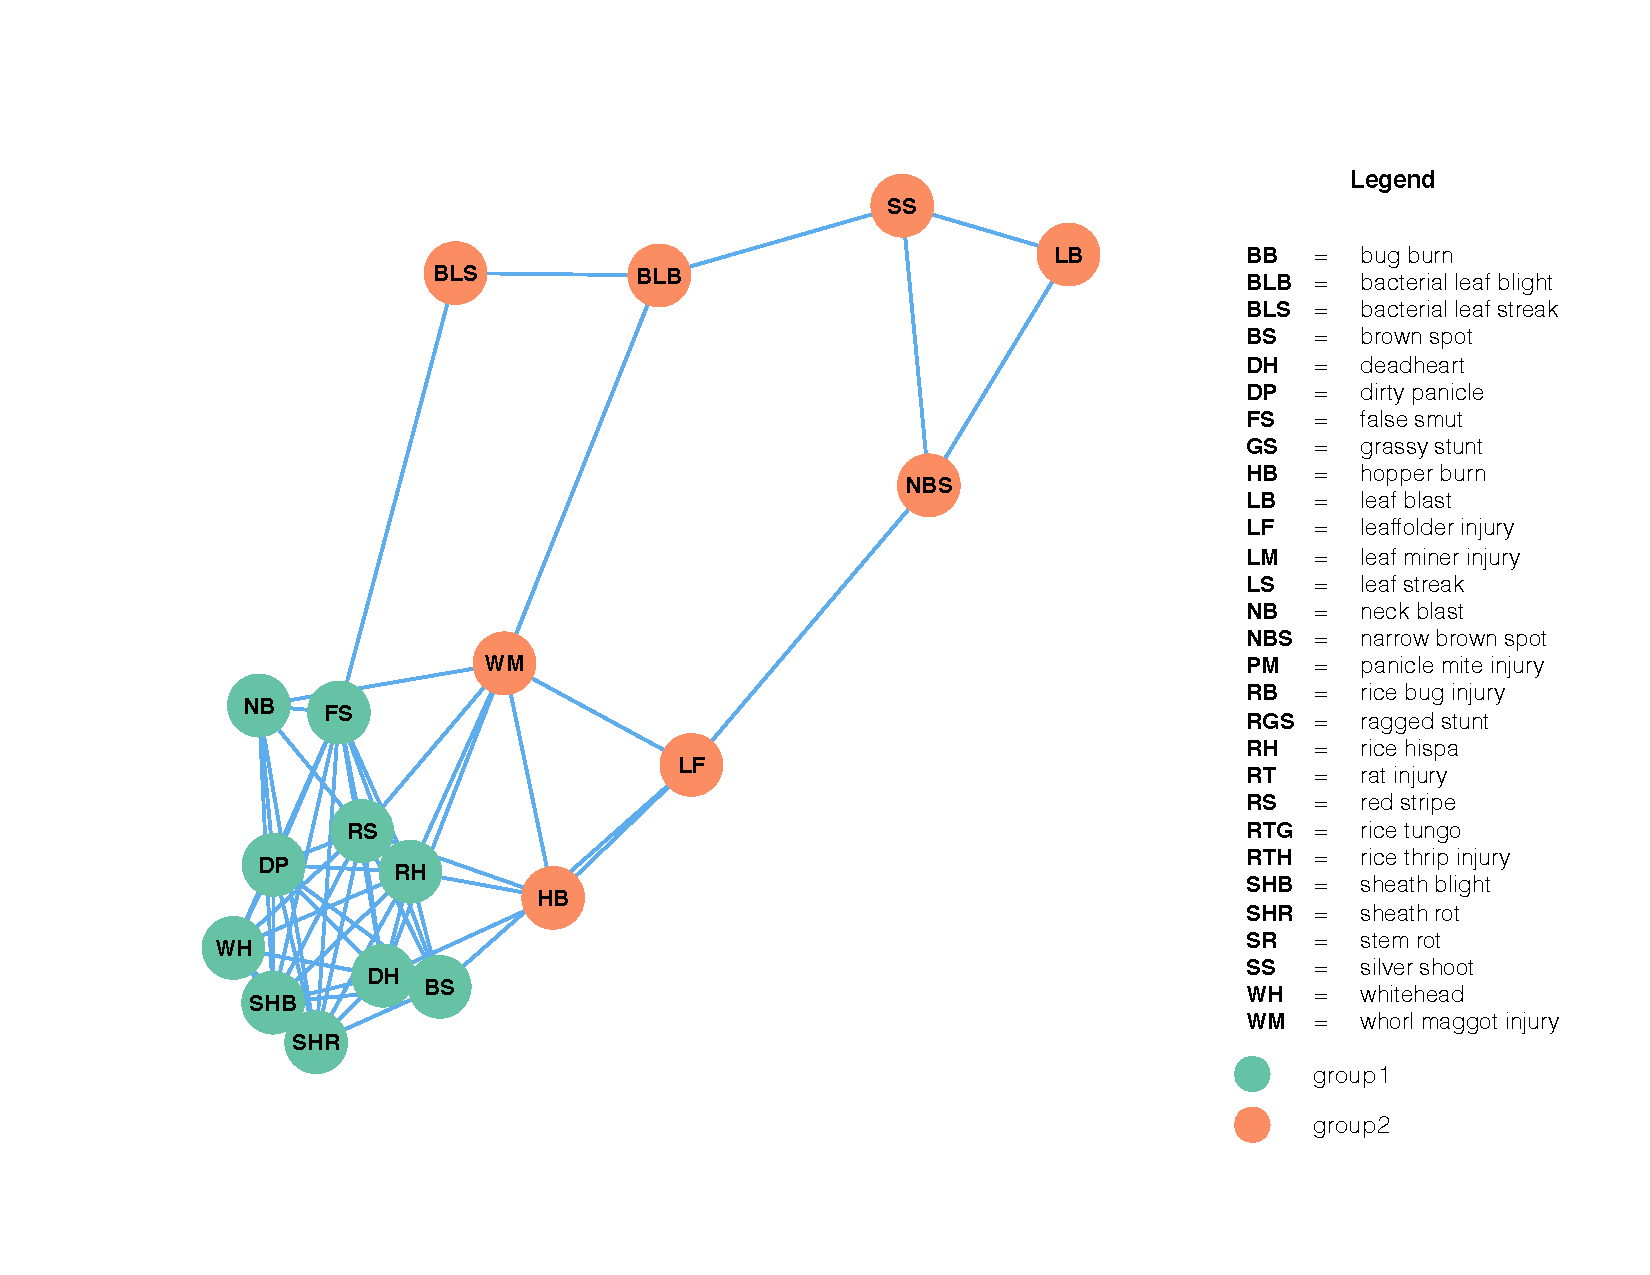
\includegraphics[width = 1\textwidth]{figures/networkCP_ds.pdf}
        \caption{Co-occurrence network of rice injuries in dry season at Central Plain, Thailand. The layout of the network graph is based on the Fruchterman-Reingold algorithm, which places nodes with stronger or more connections closer to each other.}
        \label{fig:networkCP_ds}
    \end{subfigure}
    \begin{subfigure}[b]{1\textwidth}
        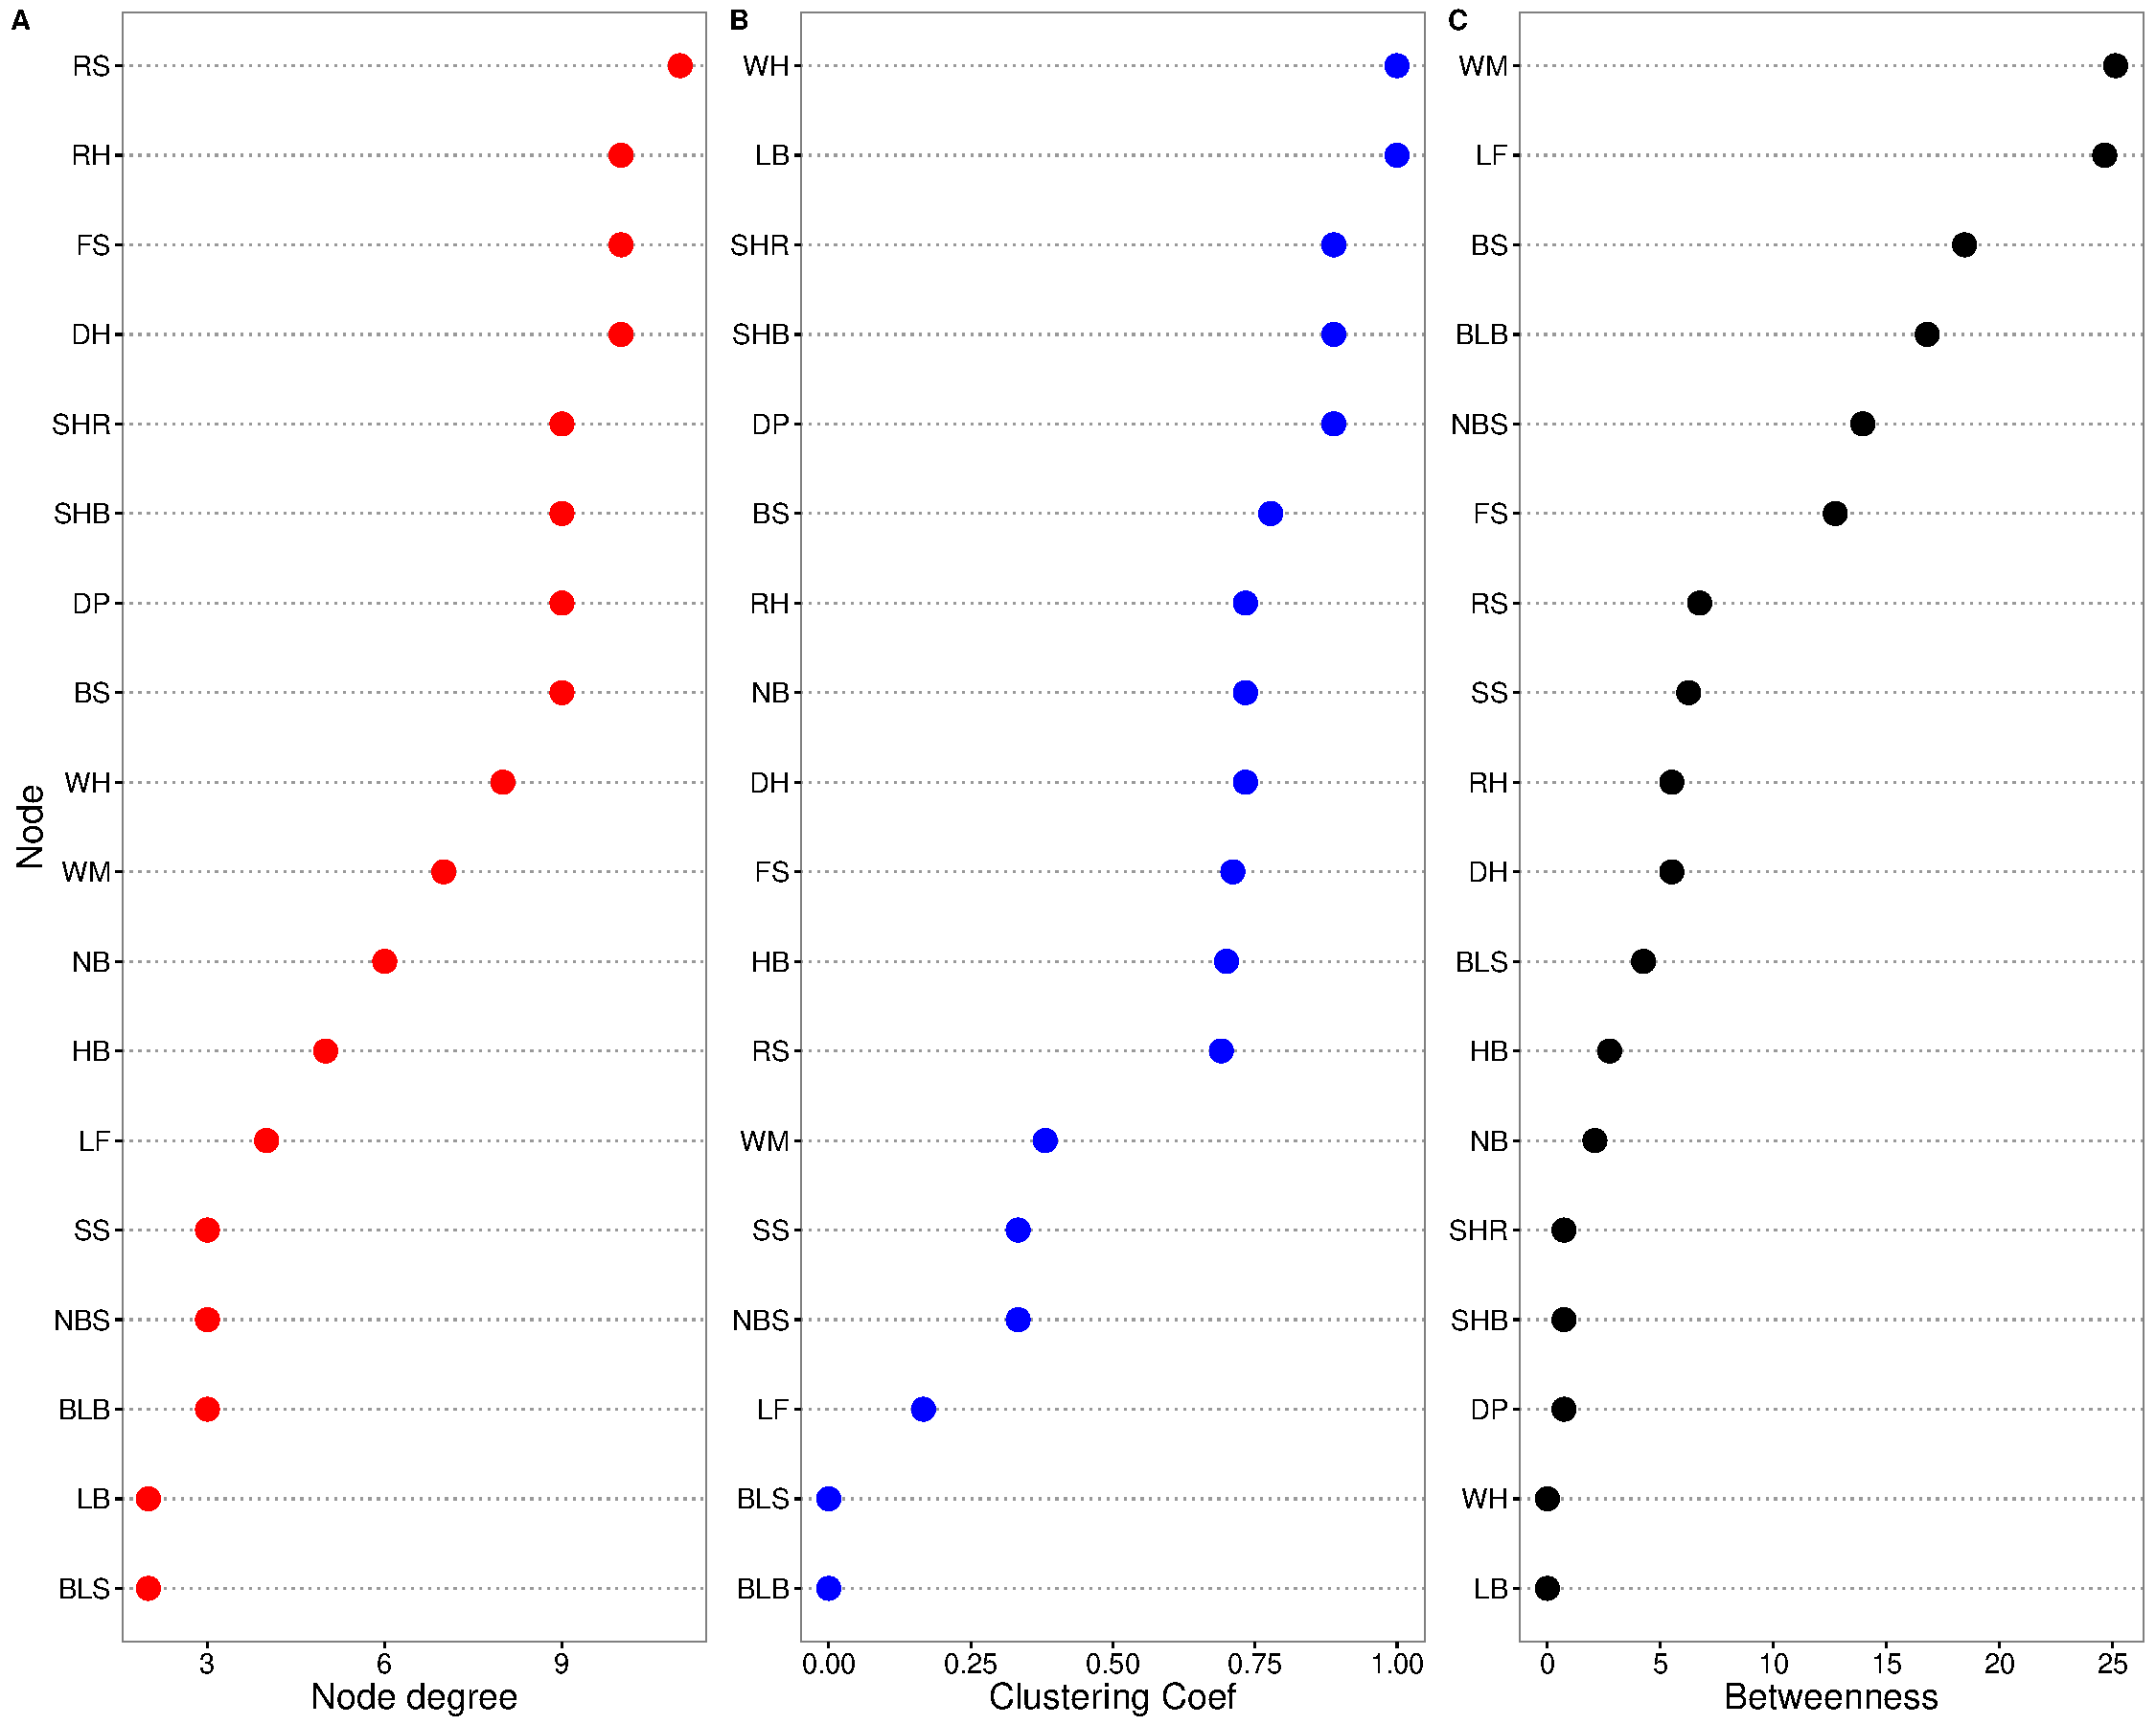
\includegraphics[width = 1\textwidth]{figures/nodepropCP_ds.pdf}
        \caption{Three centrality measures of the nodes in co-occurrence network of rice injuries in dry season at Central Plain. A: node degree, B:clustering coefficient, and C:Betweenness.}
        \label{fig:nodepropCP_ds}
    \end{subfigure}
    \caption{Rice injuries in dry season in Central Plain, Thailand}
    \label{fig:CP_ds}
\end{figure}

\begin{figure}
    \centering
    \begin{subfigure}[b]{1\textwidth}
        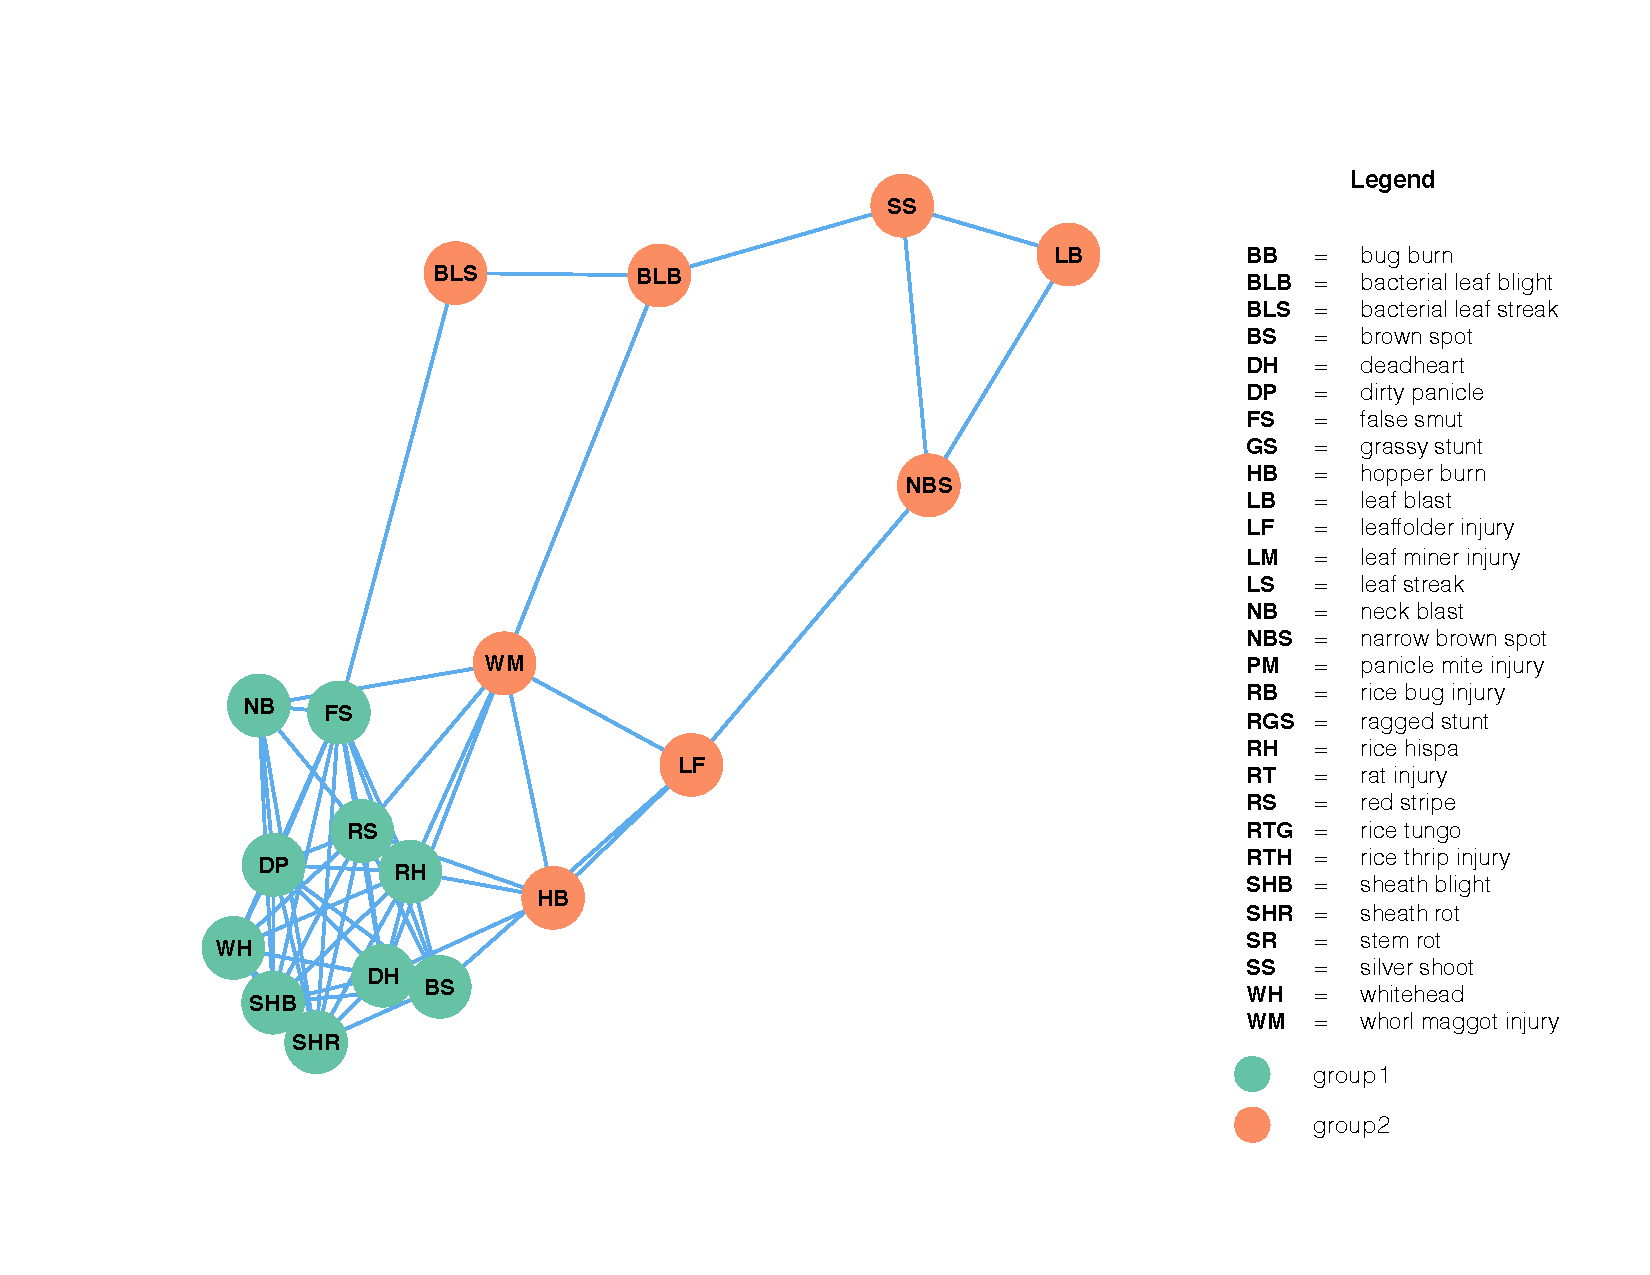
\includegraphics[width = 1\textwidth]{figures/networkCP_ws.pdf}
        \caption{Co-occurrence network of rice injuries in dry season at Central Plain, Thailand. The layout of the network graph is based on the Fruchterman-Reingold algorithm, which places nodes with stronger or more connections closer to each other.}
        \label{fig:networkCP_ws}
    \end{subfigure}
    \begin{subfigure}[b]{1\textwidth}
        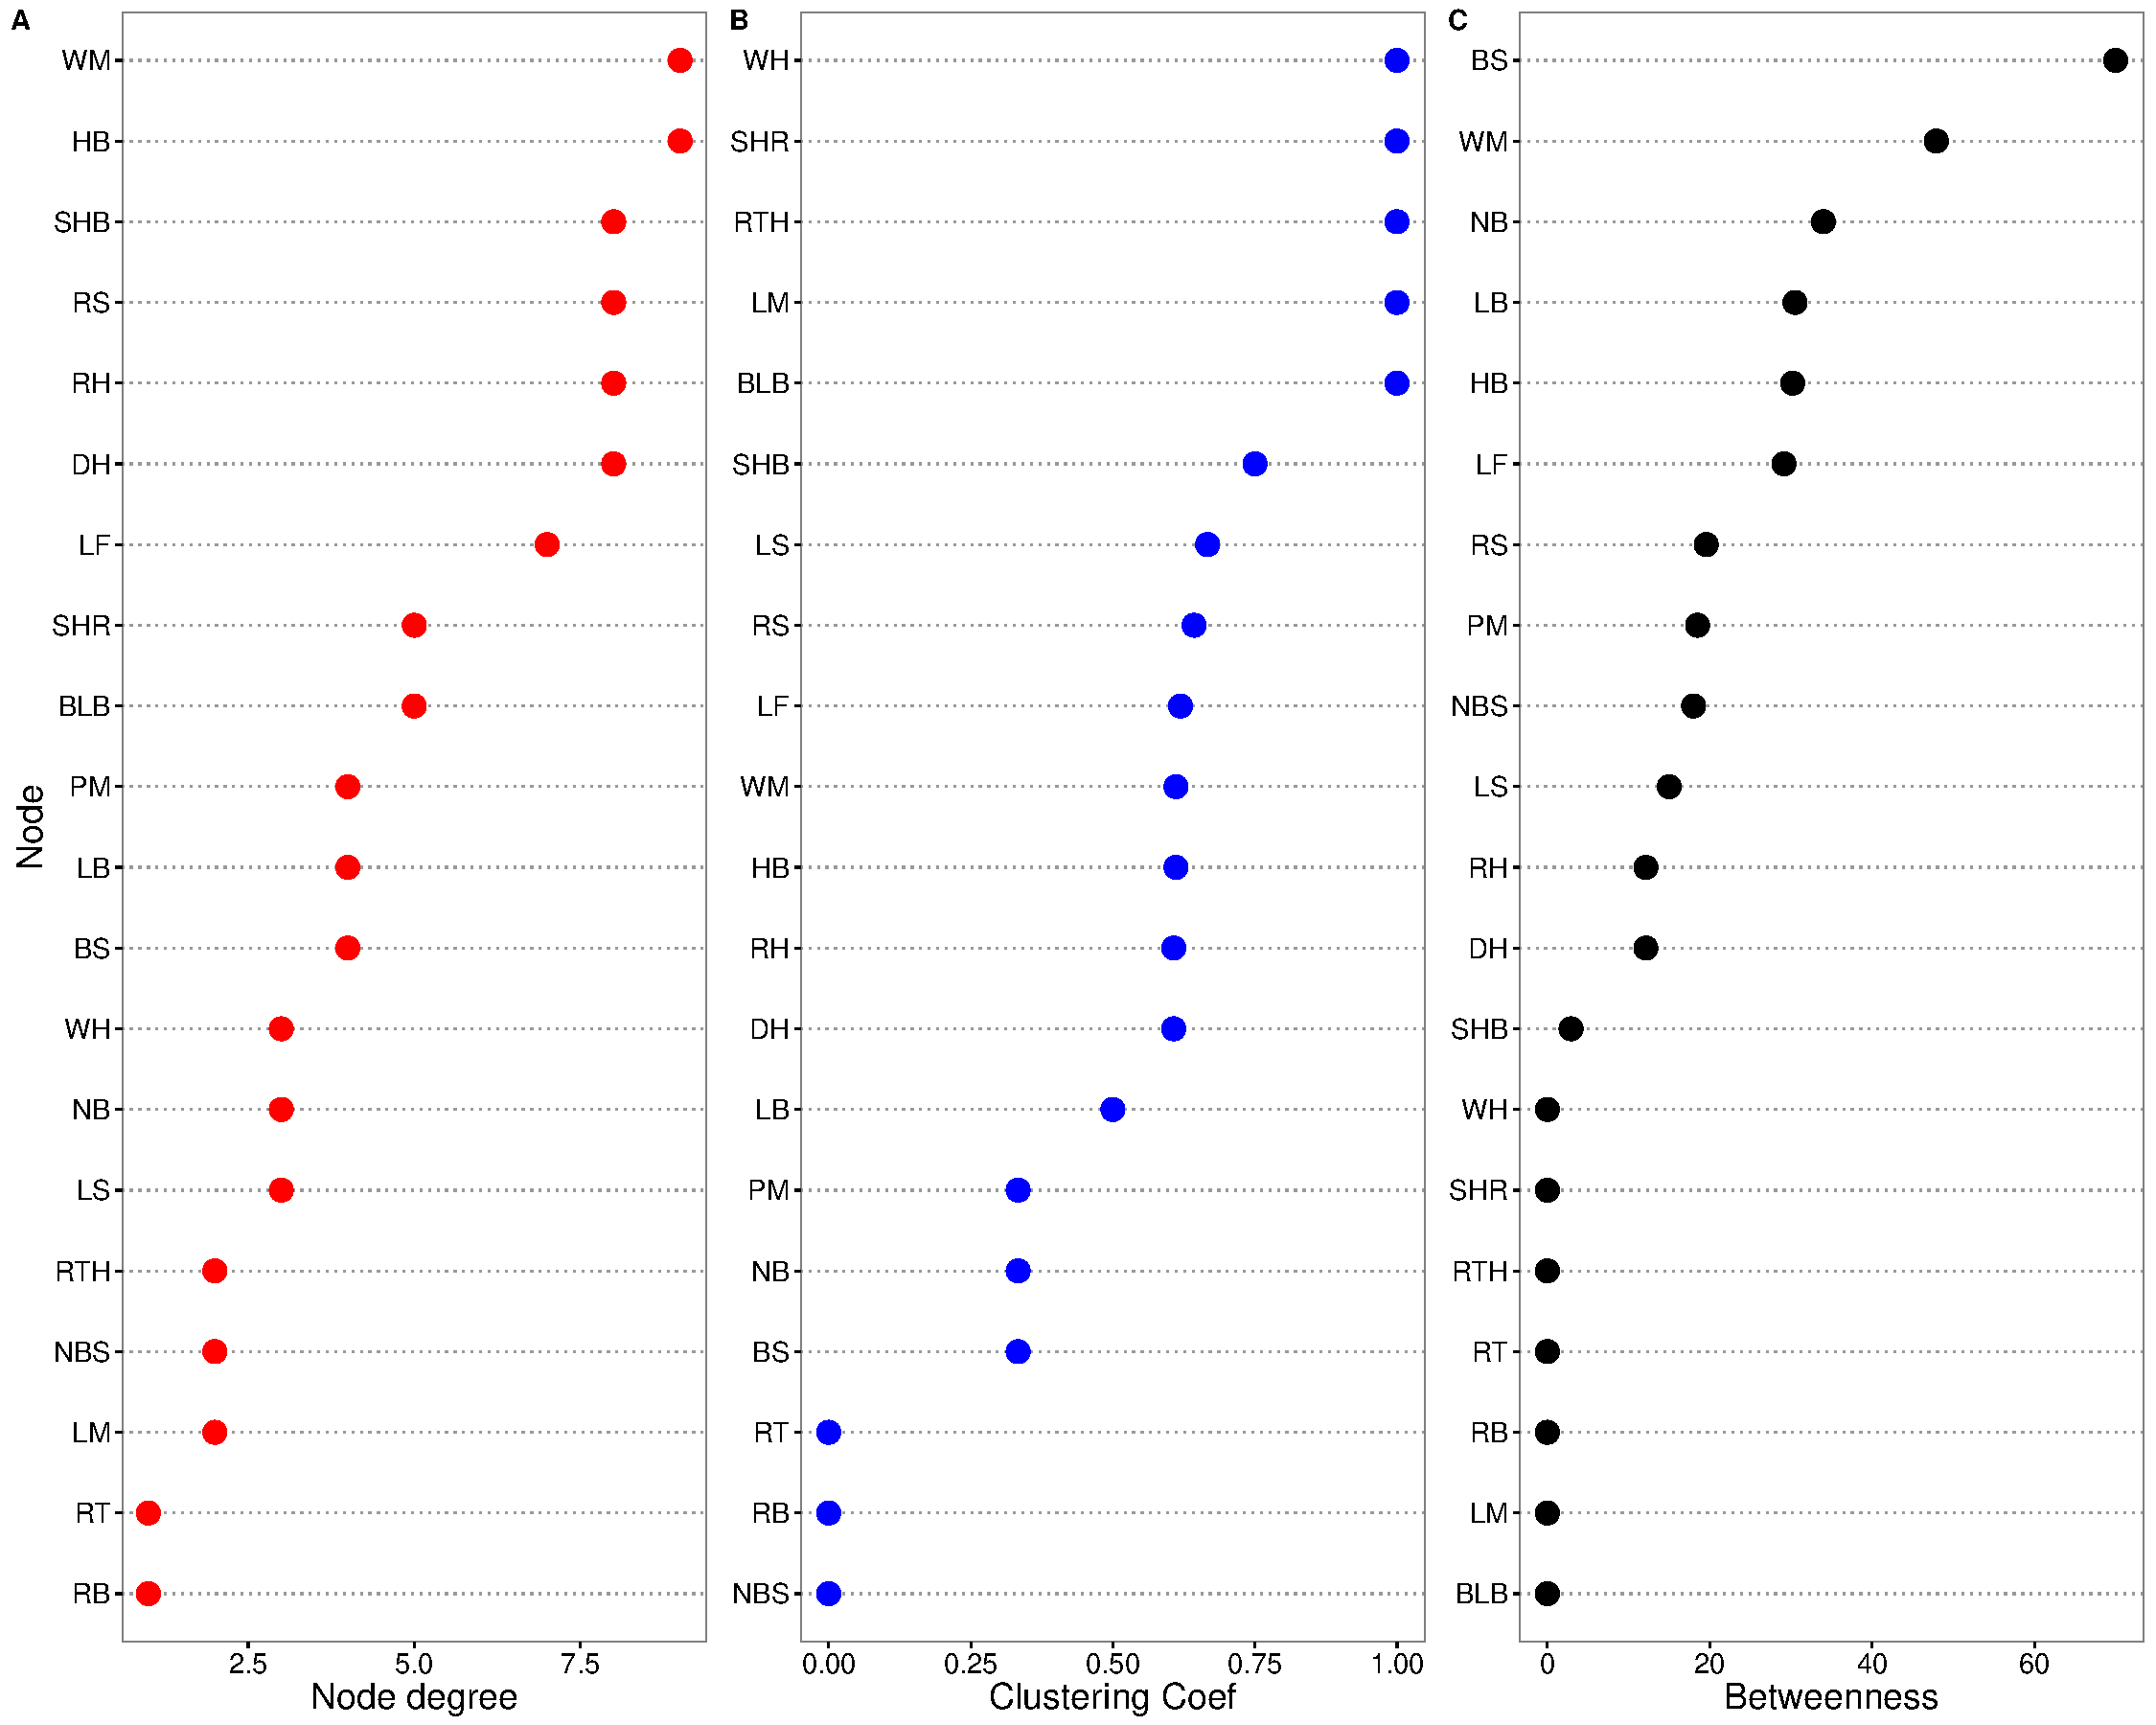
\includegraphics[width = 1\textwidth]{figures/nodepropCP_ws.pdf}
        \caption{Three centrality measures of the nodes in co-occurrence network of rice injuries in dry season at Central Plain. A: node degree, B:clustering coefficient, and C:Betweenness}
        \label{fig:nodepropCP_ds}
    \end{subfigure}
    \caption{Rice Injuries of wet season in Central Plain, Thailand}
    \label{fig:CP_ws}
\end{figure}

%\begin{figure}[p!]
%centerline{
%      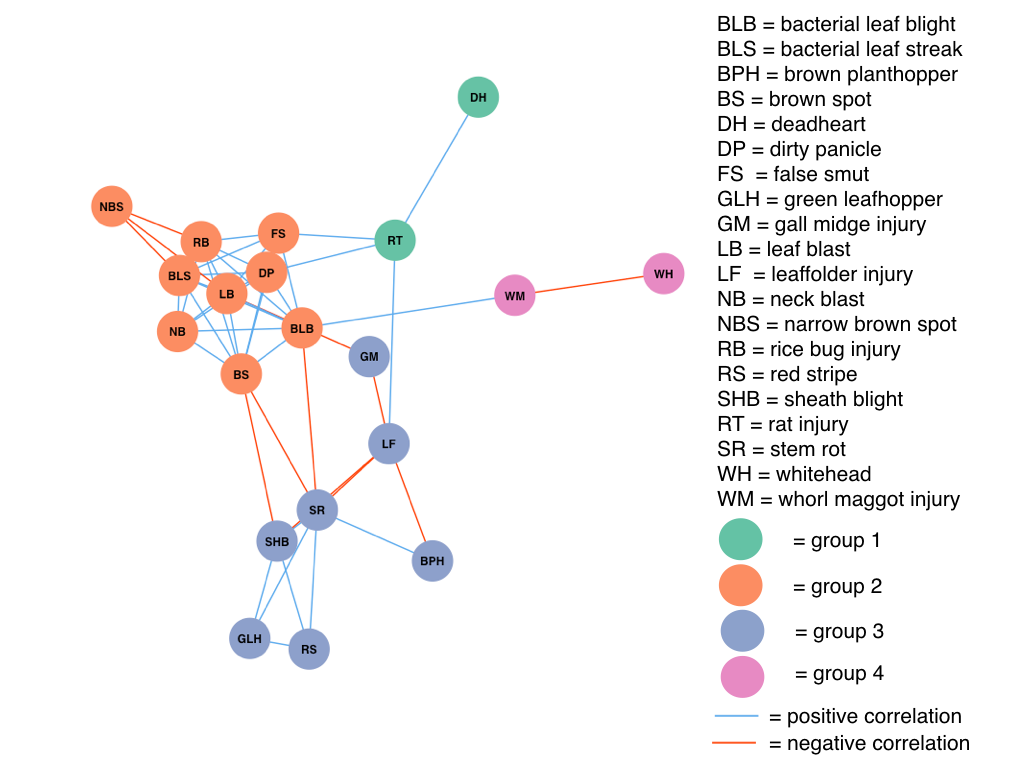
\includegraphics[width = 1\textwidth]{figures/idn_ds_net.png}
%      }
%  \caption{A picture of the same gull looking the other way!}
%\end{figure}
%
%\afterpage{\clearpage}
%\begin{figure}[p!]
%    \centering
%        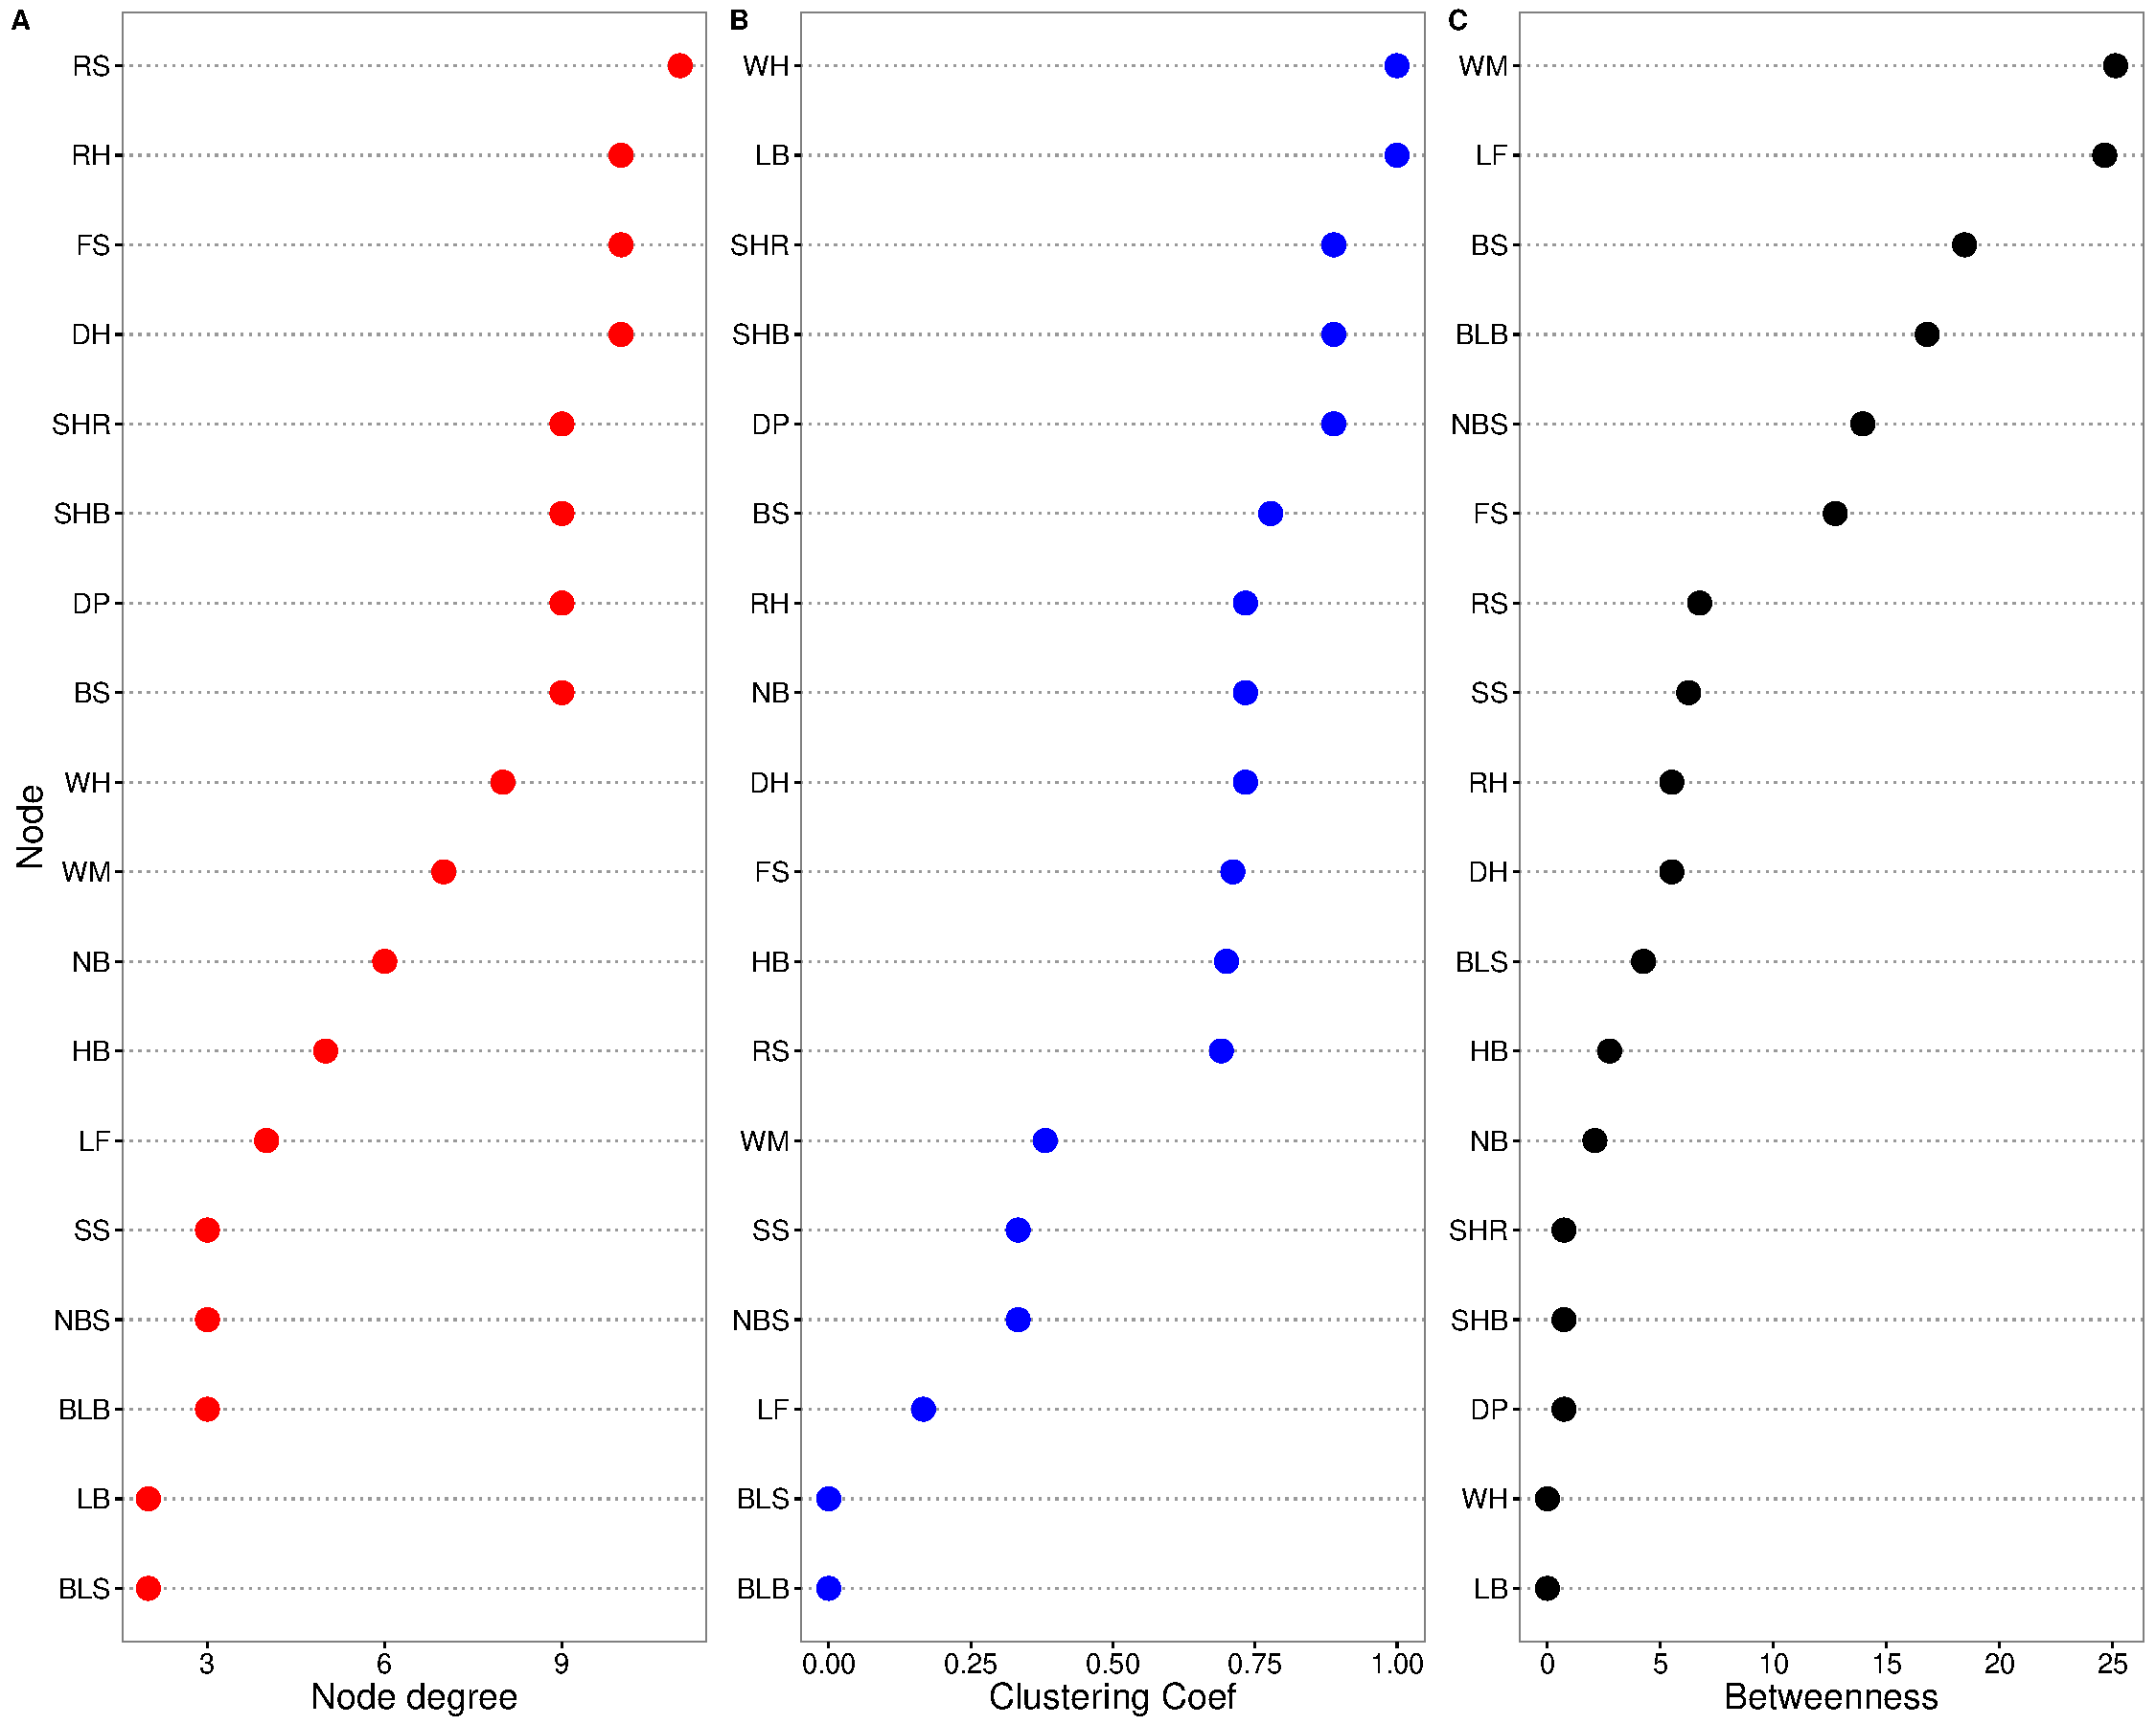
\includegraphics[width = 1\textwidth]{figures/nodepropCP_ds.pdf}
%\end{figure}

\paragraph{Odisha, India (OR)}

Dry season network (Fig) was composed of 6 associated injuries (DH, NB, SR, FS, RB, and LF) and captured 7 associations. The network showed two groups of injury syndromes (the combination of injuries). The groups of the injury profiles corresponded to each community based on the optimal clustering algorithm. The first group is composed of DH, LF, RB and SR. Another group consists of FS and NB. Analysis of network properties revealed that LF and FS are high-betweenness nodes. They presented co-occurrence relationships within group 1 and group 2. SR and RB have high clustering coefficient. It indicated that these two injuries usually formed complex of co-occurrence relationships. As opposed to other injuries, NB and DH have low scores on all three centrality measure. Apparently, these injuries less possibly co-occur with other injuries (low betweenness), and do not have complex co-occurrences with other injuries (low degree and clustering coefficient).

Wet season network (Fig) was composed of 12 nodes (injury variables, DP SR, FS, BLB, NB, LF, GLH, RT, RB, DH, WM, BPH) with edges. Fig reveals three groups of injury profiles. DH, GLH, SR and BPH are in the group 1 (green).  FS, NB, DP, BLB is in group 2 (orange). RT, LF, RB and WM are in group 3 (purple). Top four injuries with high betweenness, DP, SR, LF, and BLB, are the members of each of group. They possibly are found co-occurrence within the group and inter-groups of injury profiles. Considered in each group, DH and GLH have high clustering coefficient in the group 1. NB has high clustering coefficient in the group 2. RT has highest clustering coefficient comparing other injuries in the group 3.  Group 2 has high clustering coefficients indicating that this group is closed clustered, and the injuries in this group formed co-occurrence.  DP and SR are important as the linkage to occur with other groups of injuries profiles because of high betweenness and degree. WM, BPH have low value of the 3 local properties. It indicated that BPH and WM were less possible to occur, and present co-occurrence patterns, and when they were observed, they were also not able to relate to many injuries. 

\begin{figure}
    \centering
    \begin{subfigure}[b]{1\textwidth}
        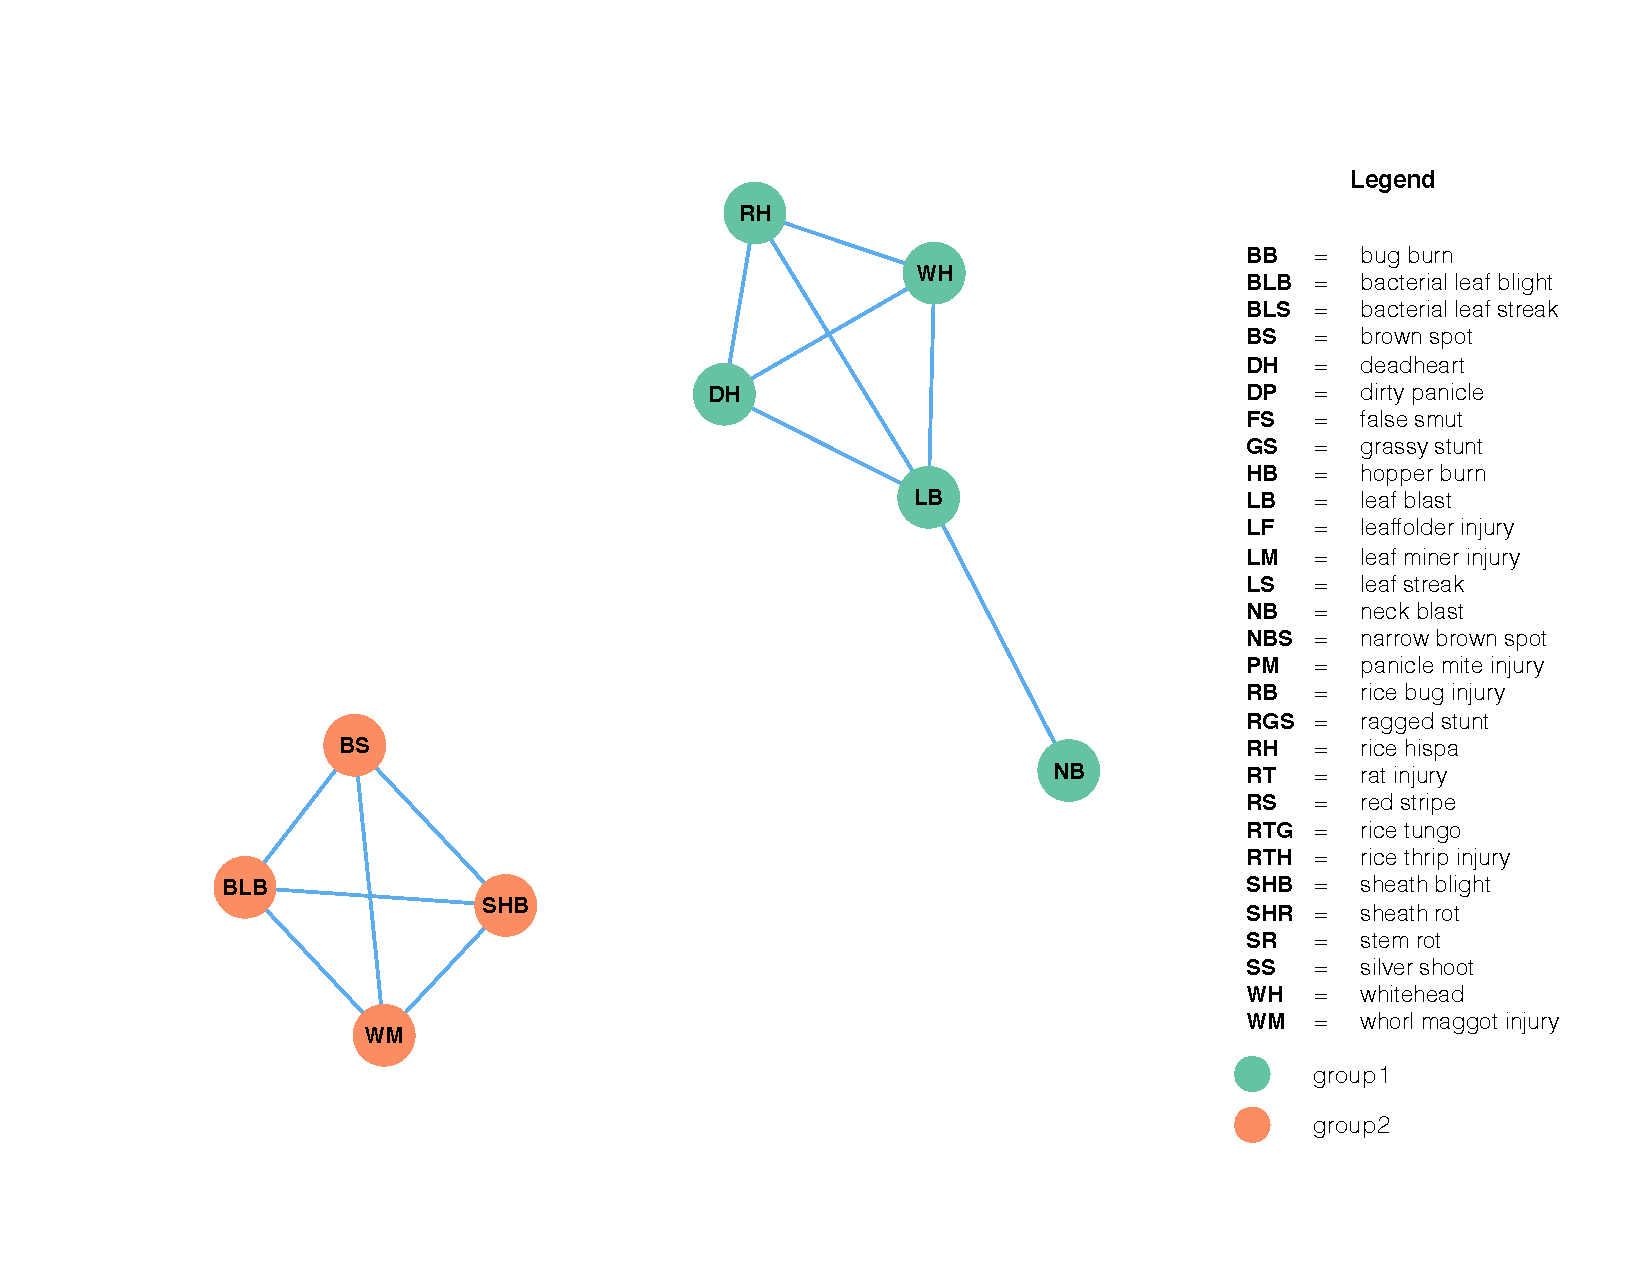
\includegraphics[width = 1\textwidth]{figures/networkOR_ds.pdf}
        \caption{Co-occurrence network of rice injuries in wet season at Odisha, India. The layout of the network graph is based on the Fruchterman-Reingold algorithm, which places nodes with stronger or more connections closer to each other.}
        \label{fig:networkOR_ds}
    \end{subfigure}
    \begin{subfigure}[b]{1\textwidth}
        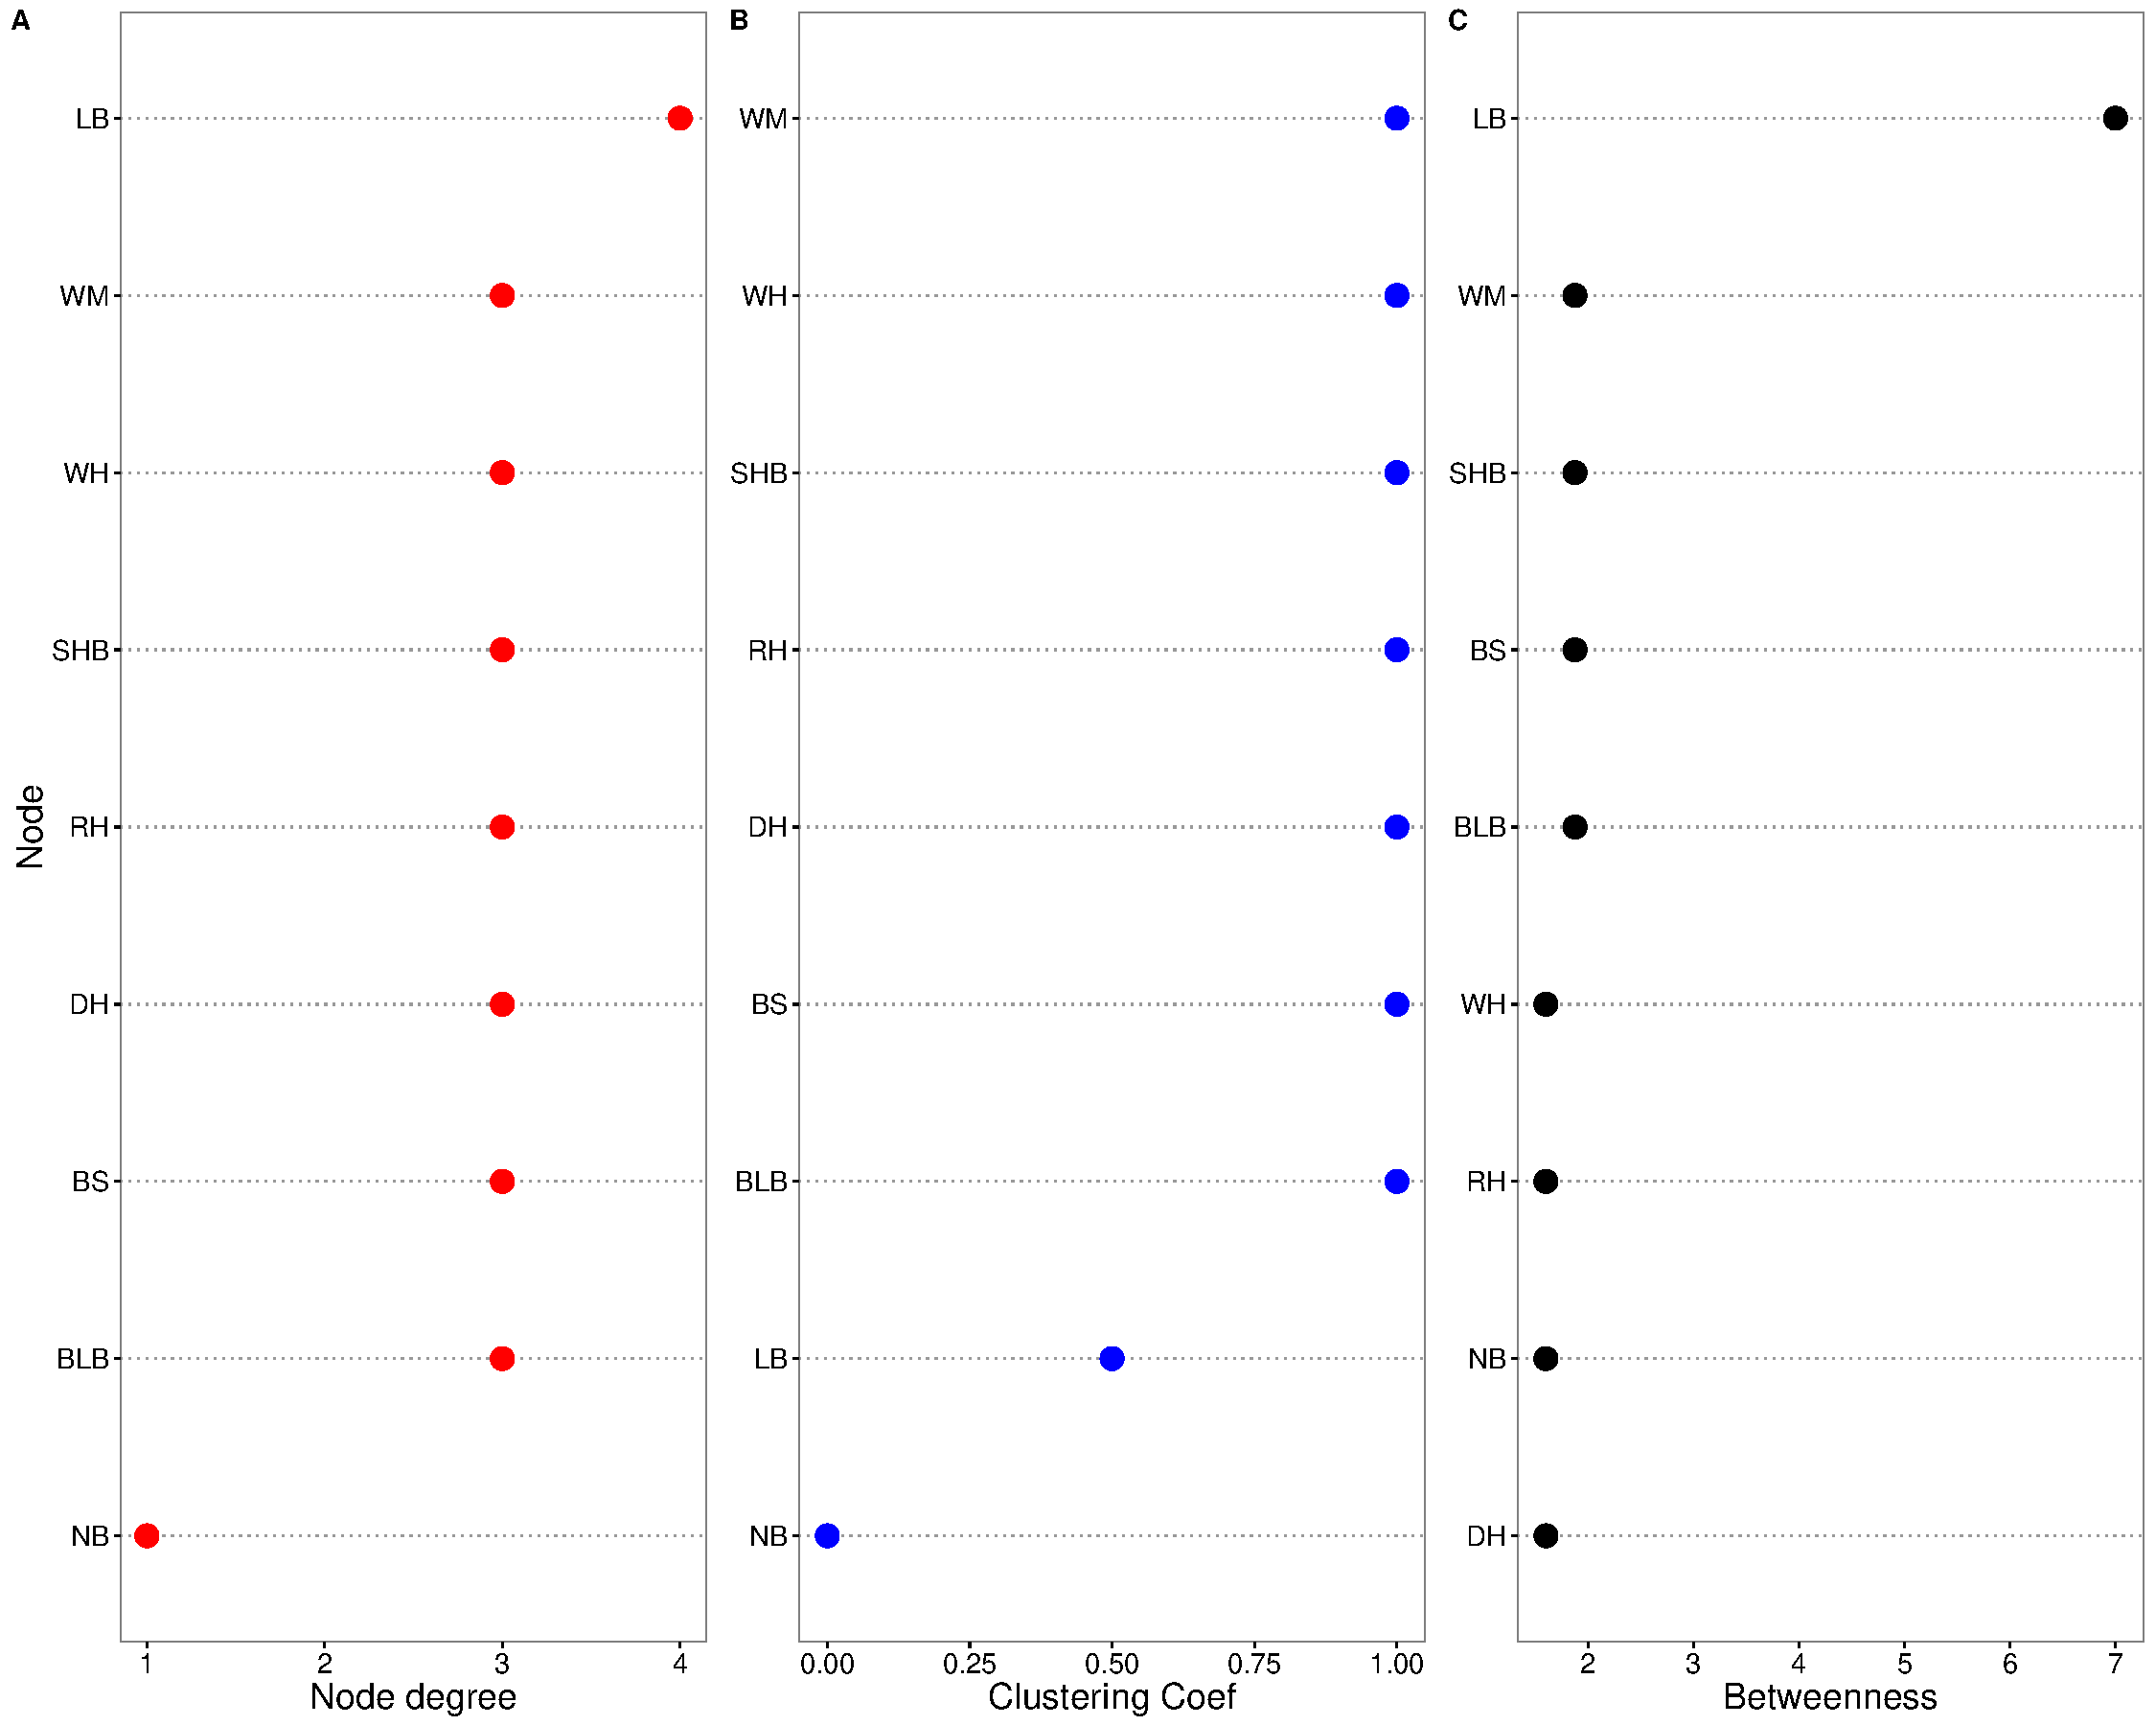
\includegraphics[width = 1\textwidth]{figures/nodepropOR_ds.pdf}
        \caption{Three centrality measures of the nodes in co-occurrence network of rice injuries in dry season at Odisha, India. A: node degree, B:clustering coefficient, and C:Betweenness, and.}
        \label{fig:nodepropCP_ds}
    \end{subfigure}
    \caption{Rice injuries in dry season at Odisha, India}
    \label{fig:OR_ds}
\end{figure}

\begin{figure}
    \centering
    \begin{subfigure}[b]{1\textwidth}
        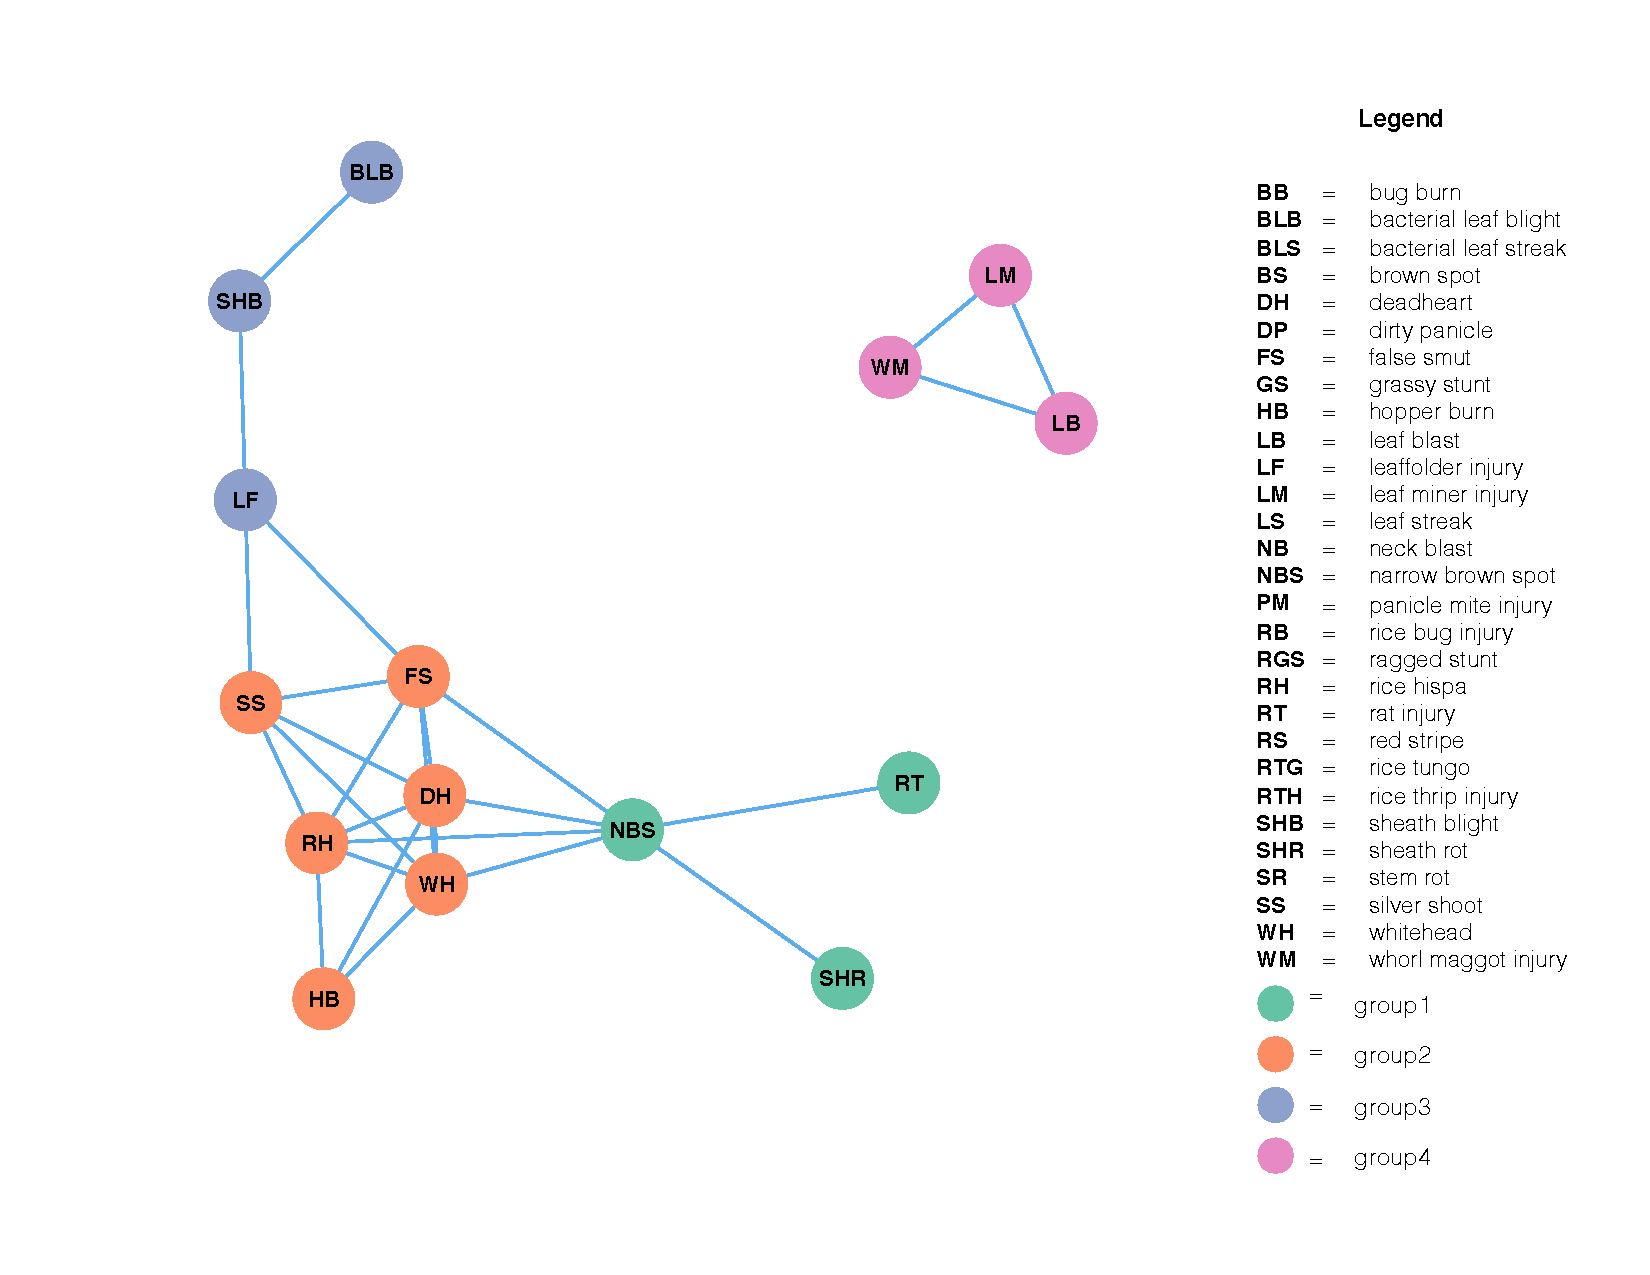
\includegraphics[width = 1\textwidth]{figures/networkOR_ws.pdf}
        \caption{Co-occurrence network of rice injuries in wet season at Odisha, India. The layout of the network graph is based on the Fruchterman-Reingold algorithm, which places nodes with stronger or more connections closer to each other.}
        \label{fig:gull}
    \end{subfigure}
    \begin{subfigure}[b]{1\textwidth}
        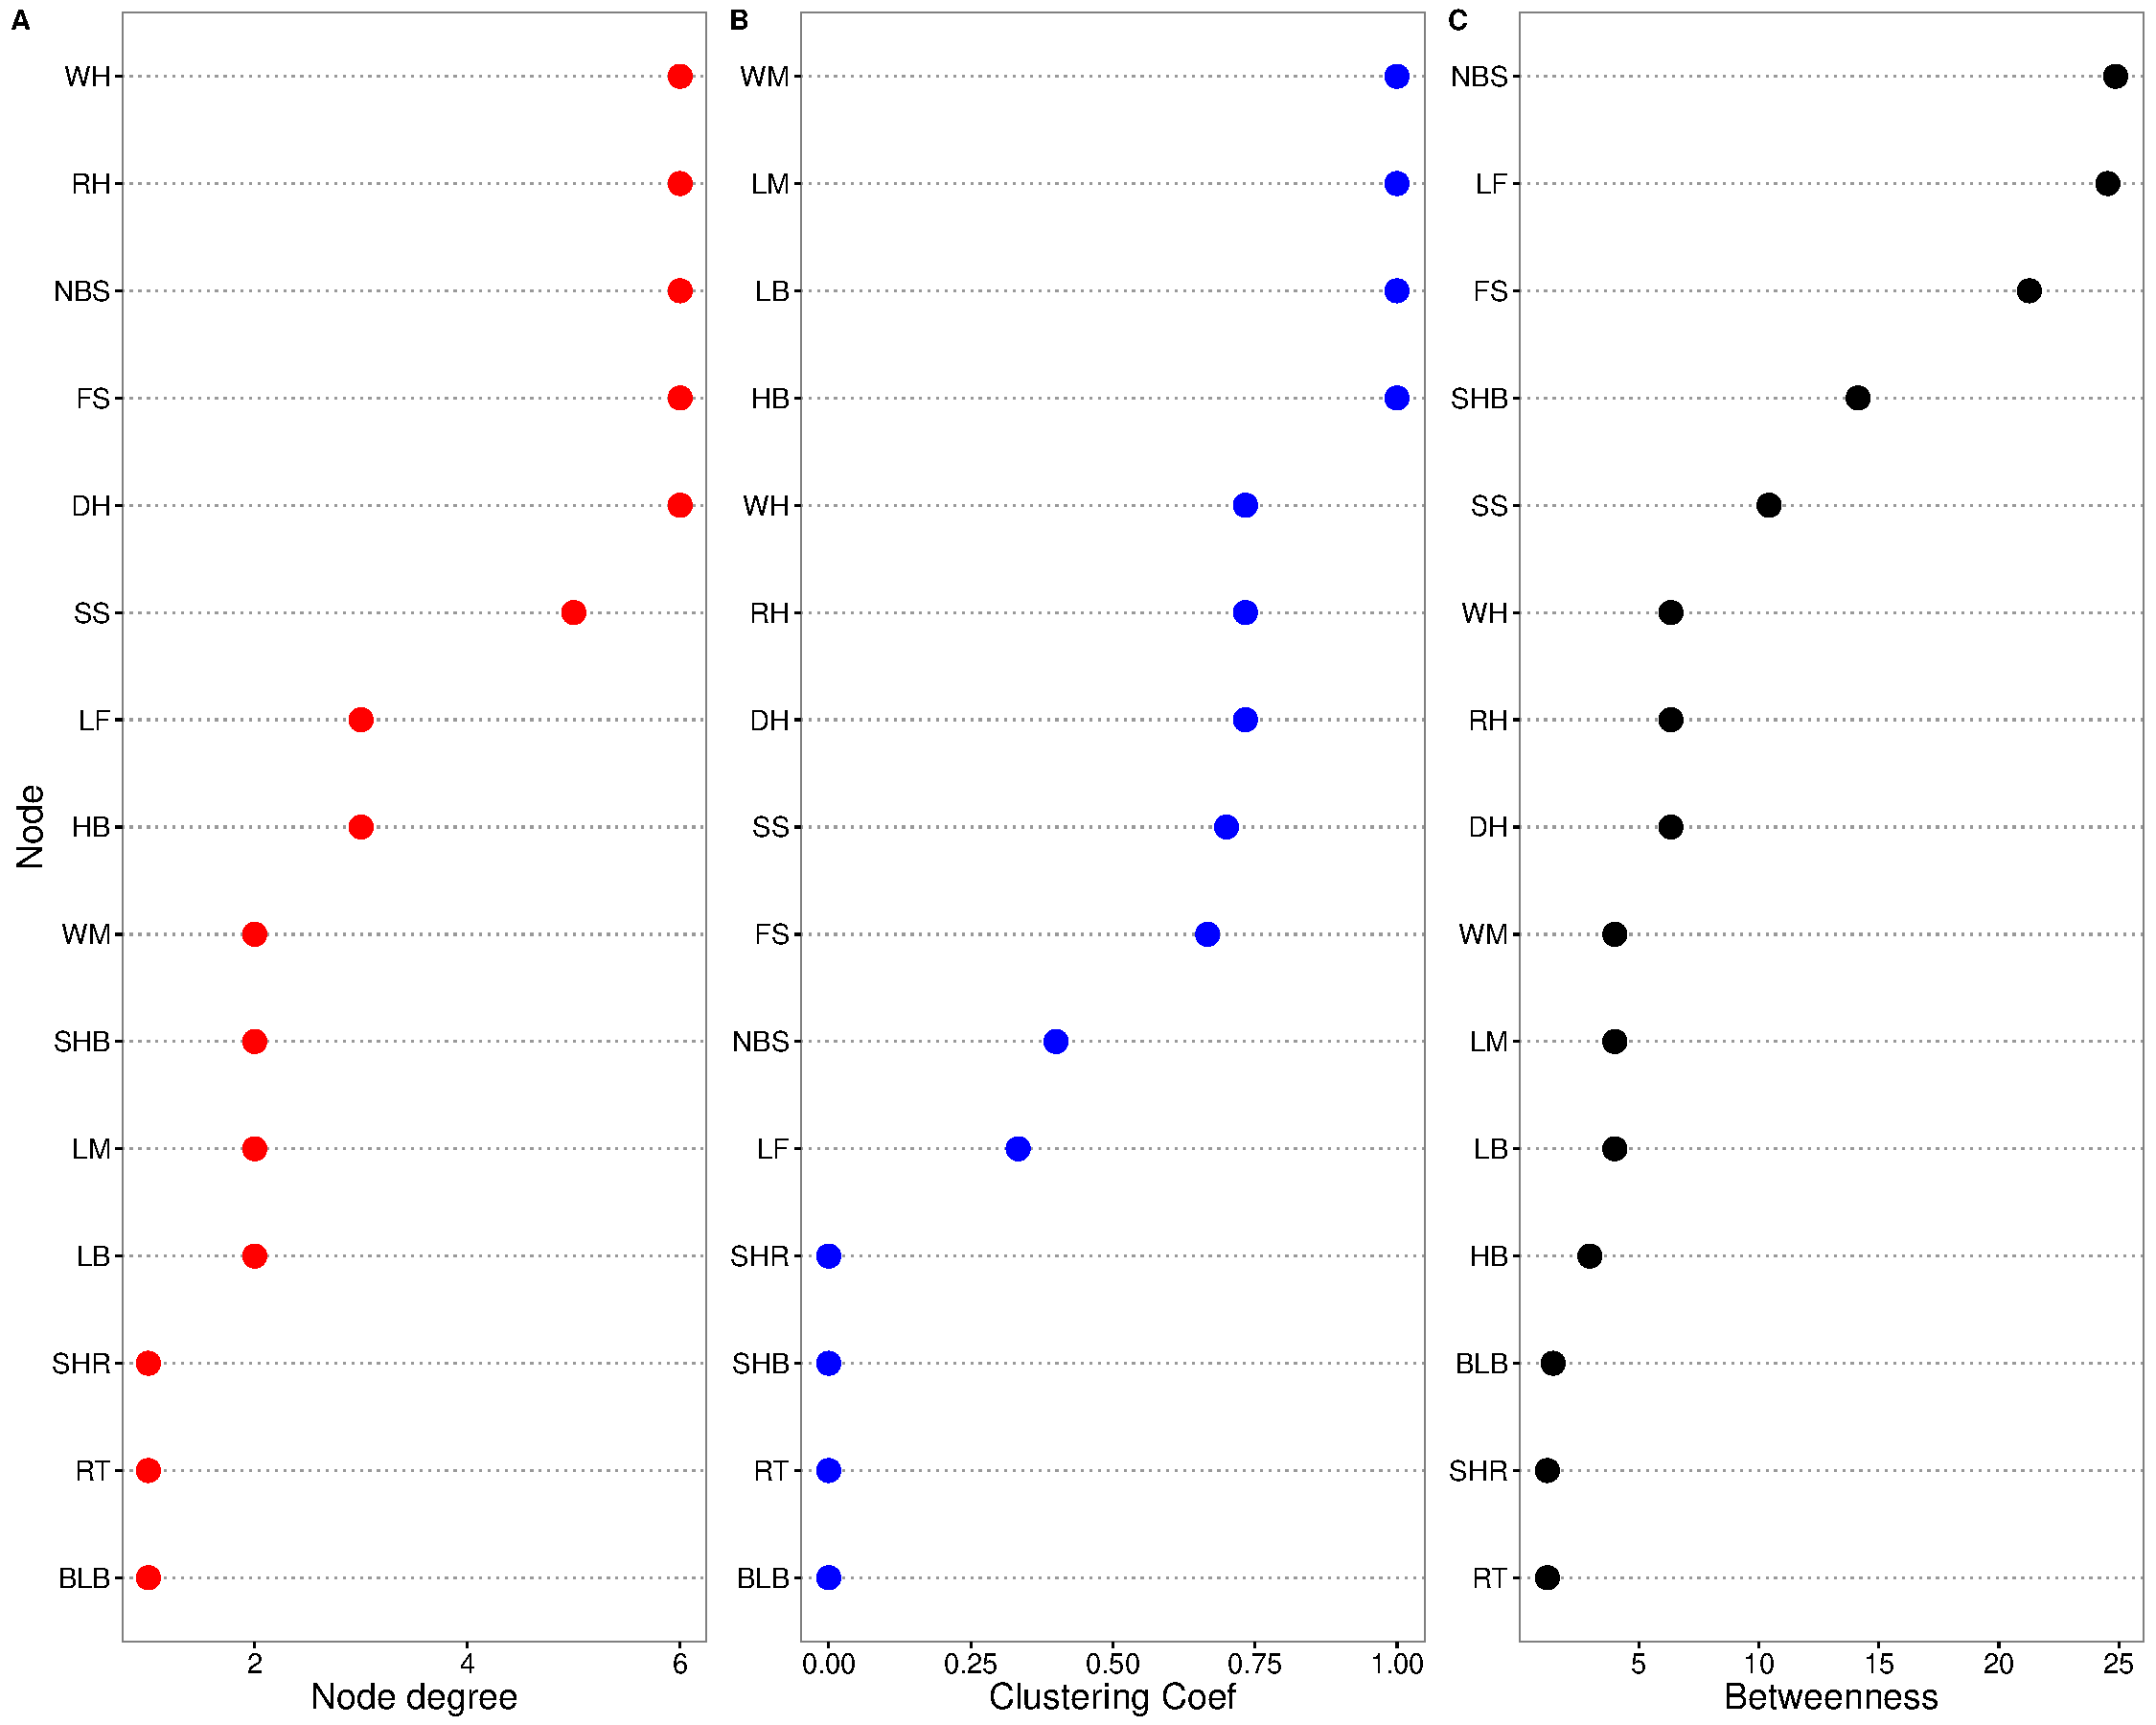
\includegraphics[width = 1\textwidth]{figures/nodepropOR_ws.pdf}
        \caption{Three centrality measures of the nodes in co-occurrence network of rice injuries in wet season at Odisha, India. A: node degree, B:clustering coefficient, and C:Betweenness, and.}
        \label{fig:nodepropCP_ds}
    \end{subfigure}
    \caption{Rice injuries in wet season at Odisha, India}
    \label{fig:OD_ws}
\end{figure}


\paragraph{West Java, Indonesia (WJV)}
 
Dry season network (Fig.) composed of 20 nodes and 51 associations. The network reveals four groups of injury profiles. Group 1 (green color) include DH and RT. Group 2 (orange color) is NBS RB, FS, BLS, LB, DP, BLB, NB, BS. Group 3 (purple color) included GM, LF, BPH, SR, SHB, GLH, RS. Group 4 (pink color) include WM and WH.  The second and third group are formed closely clusters.  RT in group 1, BLB and BS in the group 2, LF of group 3, and WM in group 4 are high-betweenness nodes with intermediate clustering coefficient.  NBS, NB, RB, BLS, FS, DP of group 2 have high clustering coefficients. Compared to group 2, the injuries in group 3 have relatively smaller than. It indicated that the injuries in the group 2 are tightly formed complex co-occurrence.  DH, WH have low value of the three features, and located far from the center of the network. BPH and WM were less possible to occur, and present co-occurrence patterns, and when they were observed, they were also not able to relate to many injuries. connectivity.

Wet season network (Fig.) composed of 19 injuries (WM, LF, GLH, DH, BLS, WH, NBS, FS, DP, RS, LB, WPH, SR, SHR, SHB, NB, BS and BLB) with 25 associations. The network was loosely connected (low clustering coefficients). It reveals 3 connected groups and one isolated group of injury profiles. Group 1 (green) DH, WM, SHB, WH, GHL, LF, LB, and RS. Group 2 (orange) is composted of WPH, SR, GM, BLS and DP. Group 3 consisted of FS, NBS, SHB, BLB. Group 4, which is isolated, is composted of BS and NB. In group 1, WM is the injuries with high betweenness, and WH is the injury with high clustering coefficient. In group 2, BLS has high betweenness, and DP has high clustering coefficient. FS in group 3 node with high betweenness and high clustering coefficient. Group 1 appeared to form complex co-occurrence patterns because the average of clustering coefficient of injuries in this group are higher than other groups of injuries.  

\begin{figure}
    \centering
    \begin{subfigure}[b]{1\textwidth}
        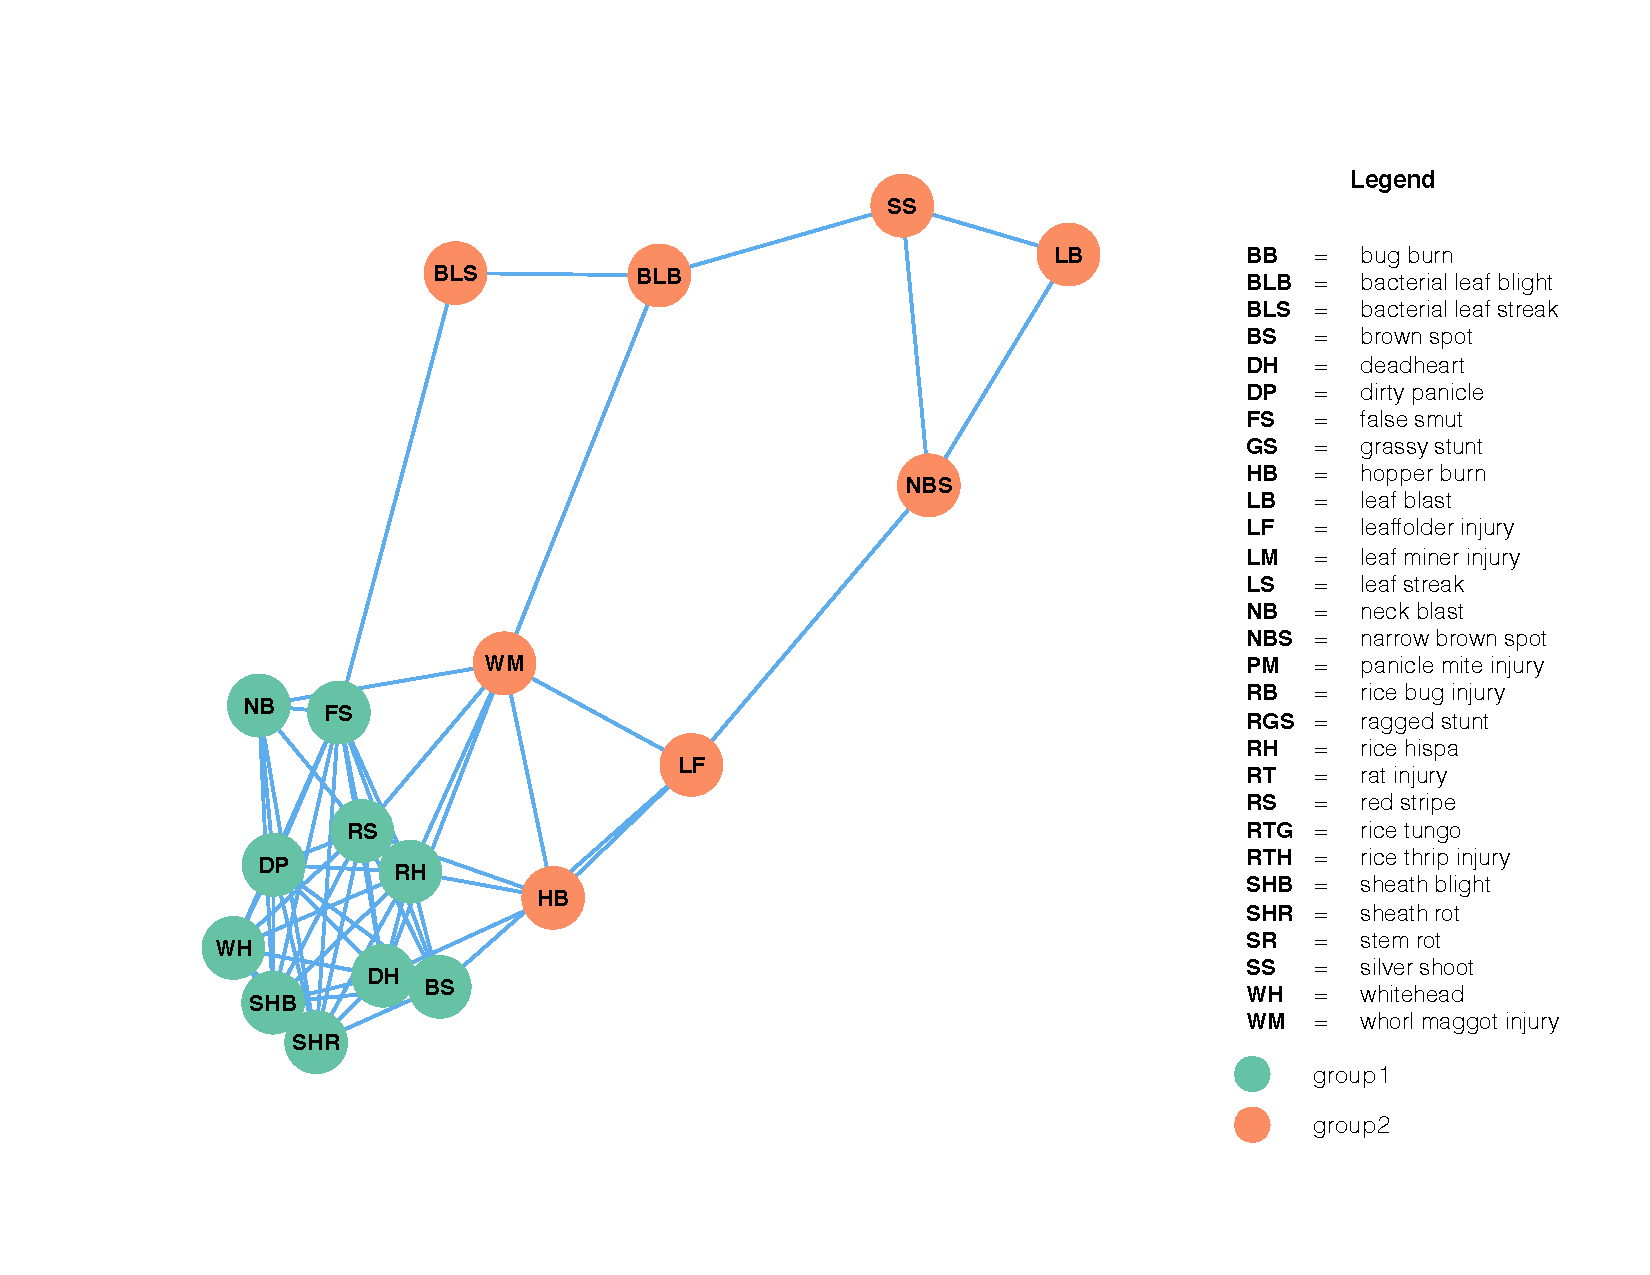
\includegraphics[width = 1\textwidth]{figures/networkRR_ds.pdf}
        \caption{Co-occurrence network of rice injuries in dry season at Red River Delta, Vietnam. The layout of the network graph is based on the Fruchterman-Reingold algorithm, which places nodes with stronger or more connections closer to each other.}
        \label{fig:networkRR_ds}
    \end{subfigure}
    \begin{subfigure}[b]{1\textwidth}
        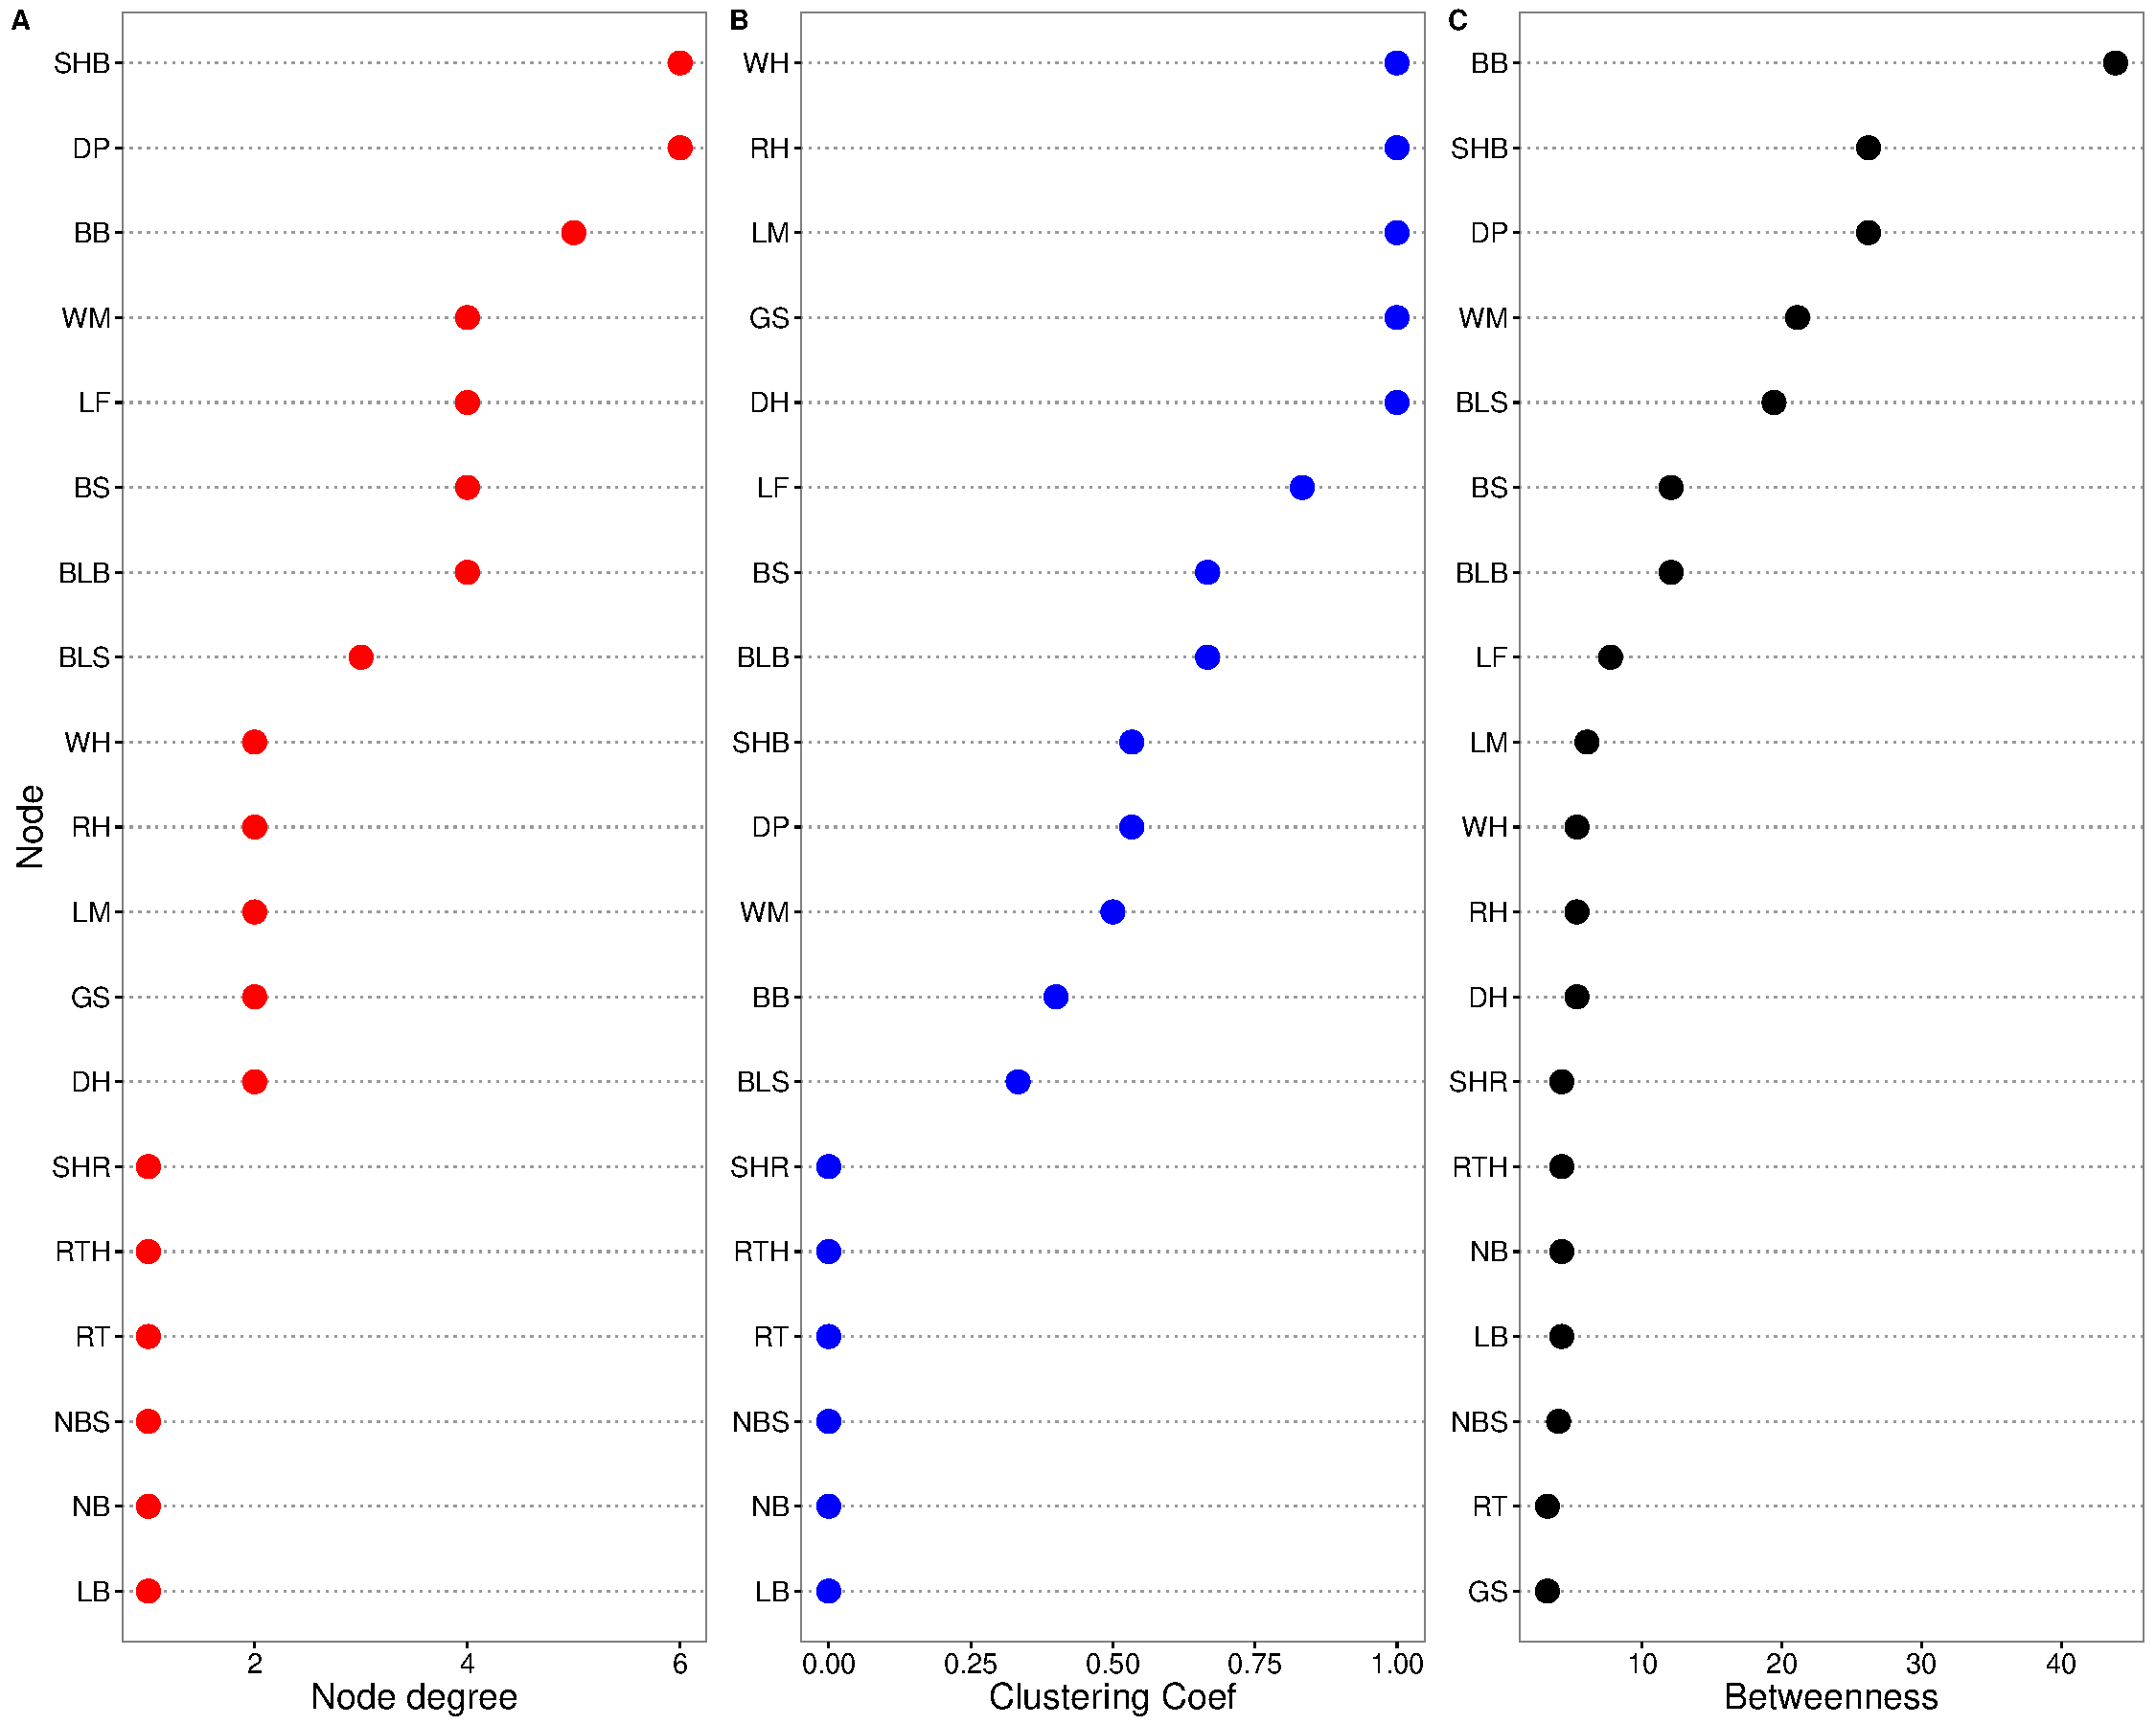
\includegraphics[width = 1\textwidth]{figures/nodepropRR_ds.pdf}
        \caption{Three centrality measures of the nodes in co-occurrence network of rice injuries in dry season at Red River Delta, Vietnam. A: node degree, B:clustering coefficient, and C:Betweenness}
        \label{fig:nodepropCP_ds}
    \end{subfigure}
    \caption{PRice injuries in wet season at Red River Delta, Vietnam}
    \label{fig:nodepropRR_ds}
\end{figure}

\begin{figure}
    \centering
    \begin{subfigure}[b]{1\textwidth}
        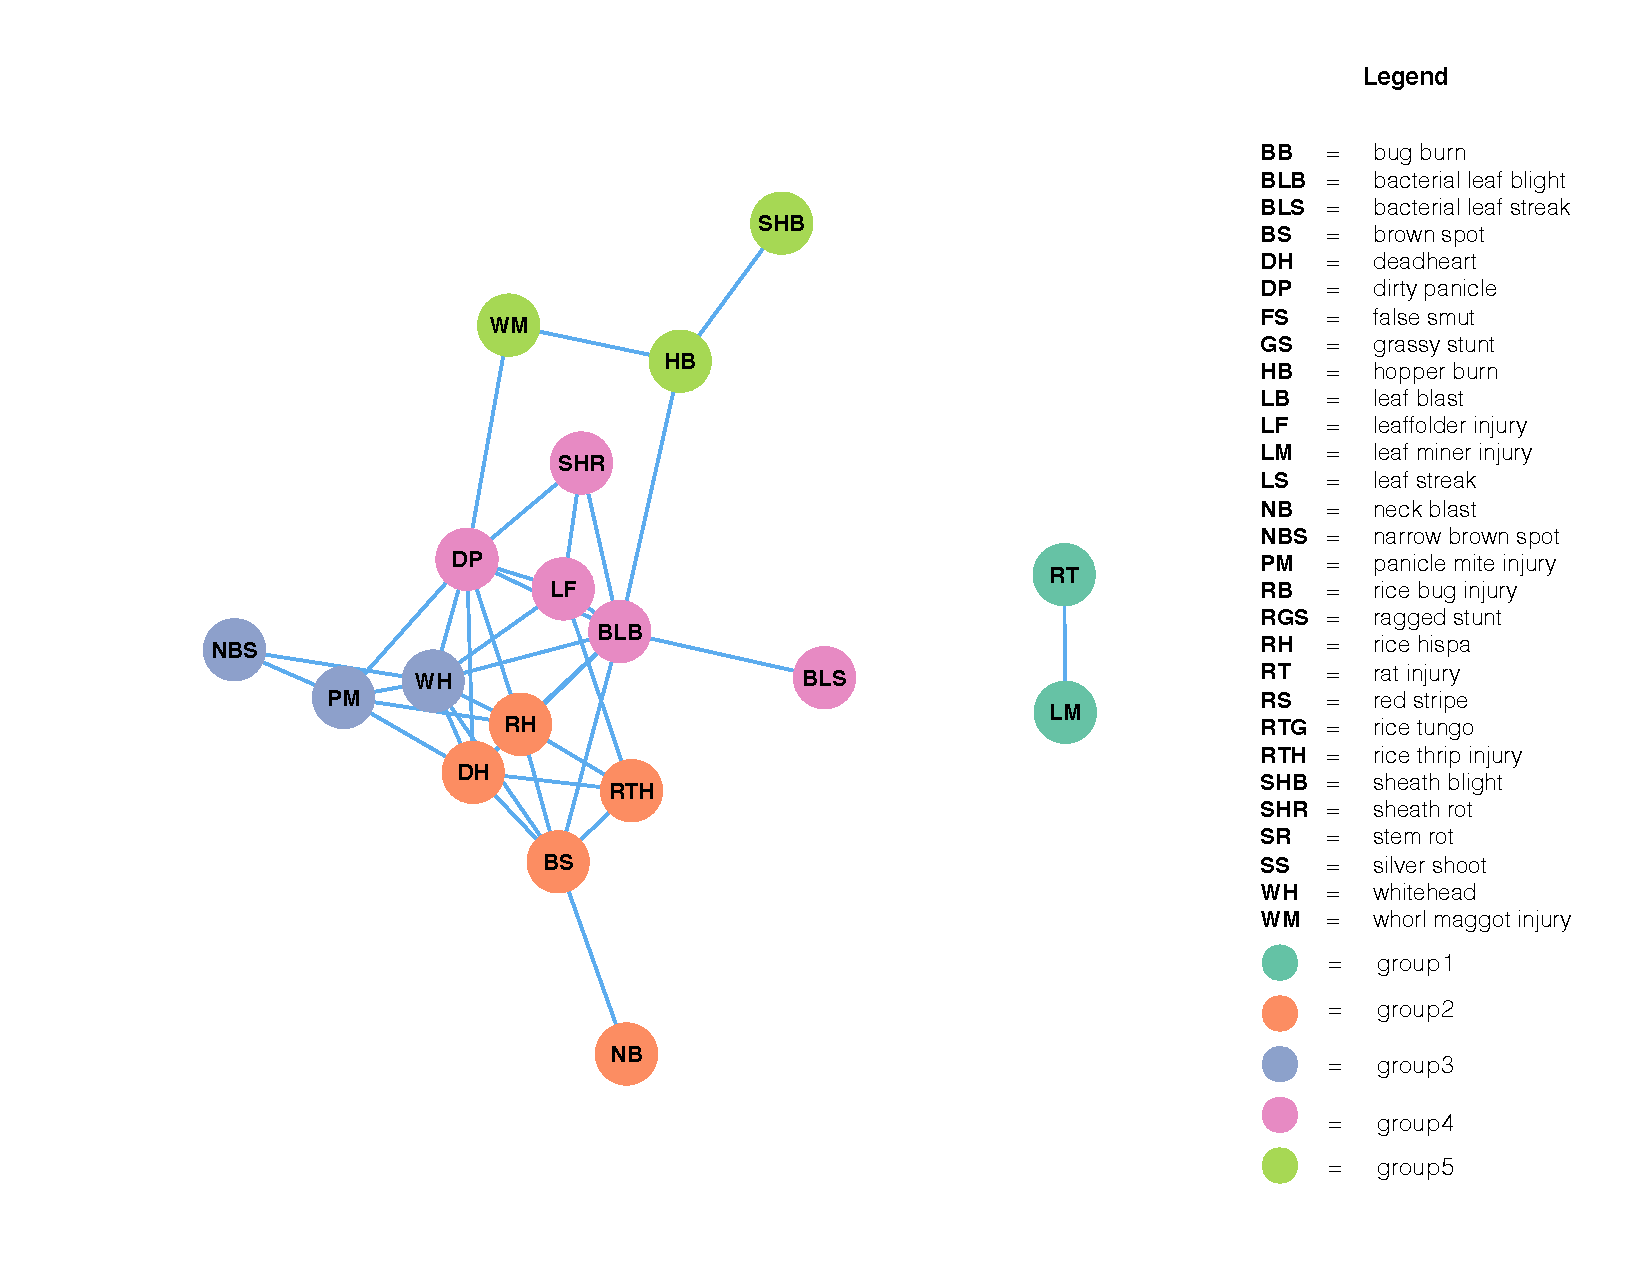
\includegraphics[width = 1\textwidth]{figures/networkRR_ws.pdf}
        \caption{Co-occurrence network of rice injuries in wet season at Red River Delta, Vietnam. The layout of the network graph is based on the Fruchterman-Reingold algorithm, which places nodes with stronger or more connections closer to each other.}
        \label{fig:networkRR_ws}
    \end{subfigure}
    \begin{subfigure}[b]{1\textwidth}
        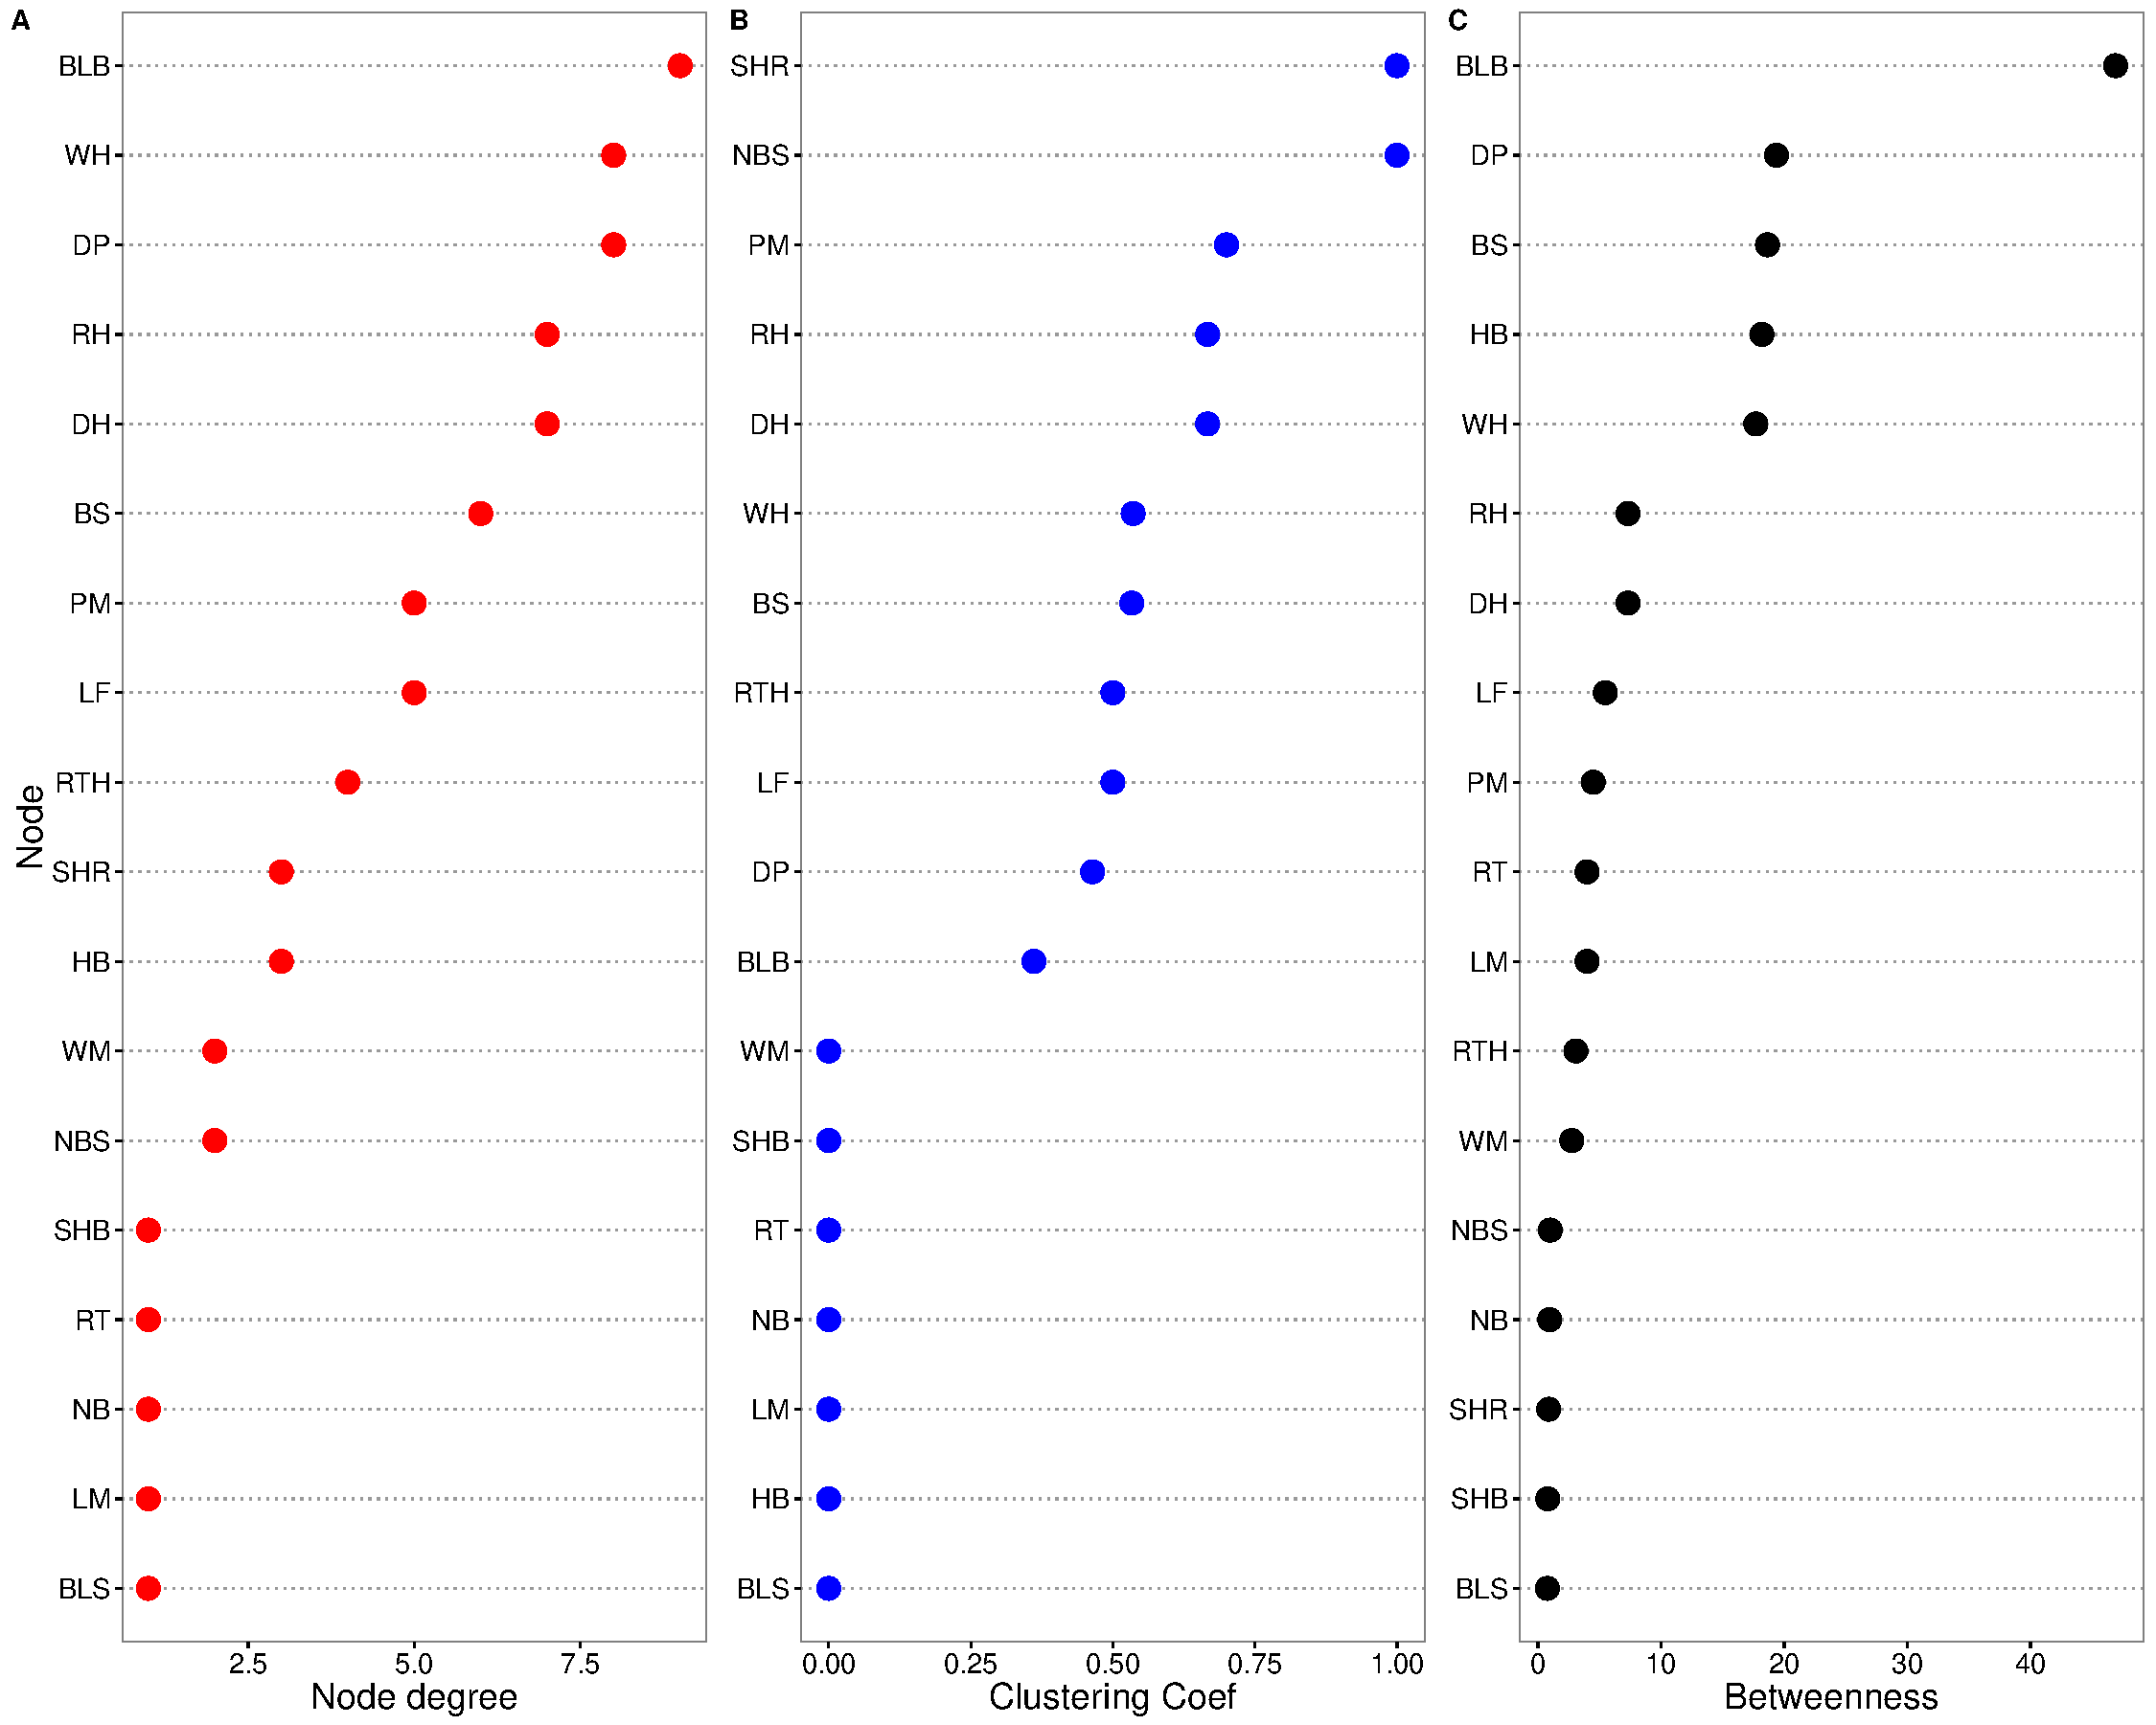
\includegraphics[width = 1\textwidth]{figures/nodepropRR_ws.pdf}
        \caption{Three centrality measures of the nodes in co-occurrence network of rice injuries in wet season at Red River Delta, Vietnam. A: node degree, B:clustering coefficient, and C:Betweenness}
        \label{fig:nodepropRR_ws}
    \end{subfigure}
    \caption{Rice injuries in wet season at Red River Delta, Vietnam}
    \label{fig:nodepropRR_ws}
\end{figure}


\paragraph{Central Luzon, Philippines (LAG)}

The dry season network reveal three clustered groups of injury profiles. Group 1 composted of WM, RB, NB, SHB, and FS. WM and RB in this group have high rank of betweenness. Group 2 consist of LB and DP. DP in this group connected with BPH (high betweenness) from group 3, which have GLH, BPH and BLB. Interestingly, SHB in group1, and GLH in group 3 have high clustering coefficients. NB, LB, FS, and BLB featured low in three of centrality. 

Figure revealed co-occurrence network of injury profiles in dry season at Laguna, the Philippines. Network resulted four groups of injury profiles, which there are three connected and one isolated. Group 1 (green) has  SHR, RS, RT, which is isolated. Group 2 (orange) has NB, RB, GLH, BLS, and DP. This group has more more complex combination than others because the clustering coefficients of injuries in this group are higher. Group 3 (purple) has LB, SHB, LB. This group is between group1 and group 4 (pink), which has NBS, LF, BS, and BLB. The position of SHB, LB and WM in the group with high betweenness, but they do not form the the complex combination of the injuries. They tend to link the co-occurrence of the first and the fourth group of injury profiles, which connected to NB in the first group and LF in the fourth group. So they are potentially good target to be monitored too. For example, when LF presented without the present of LB, SHB, WM, it is less likely NB would present, and other injuries in the first group would less likely to present neither. 

\begin{figure}
    \centering
    \begin{subfigure}[b]{1\textwidth}
        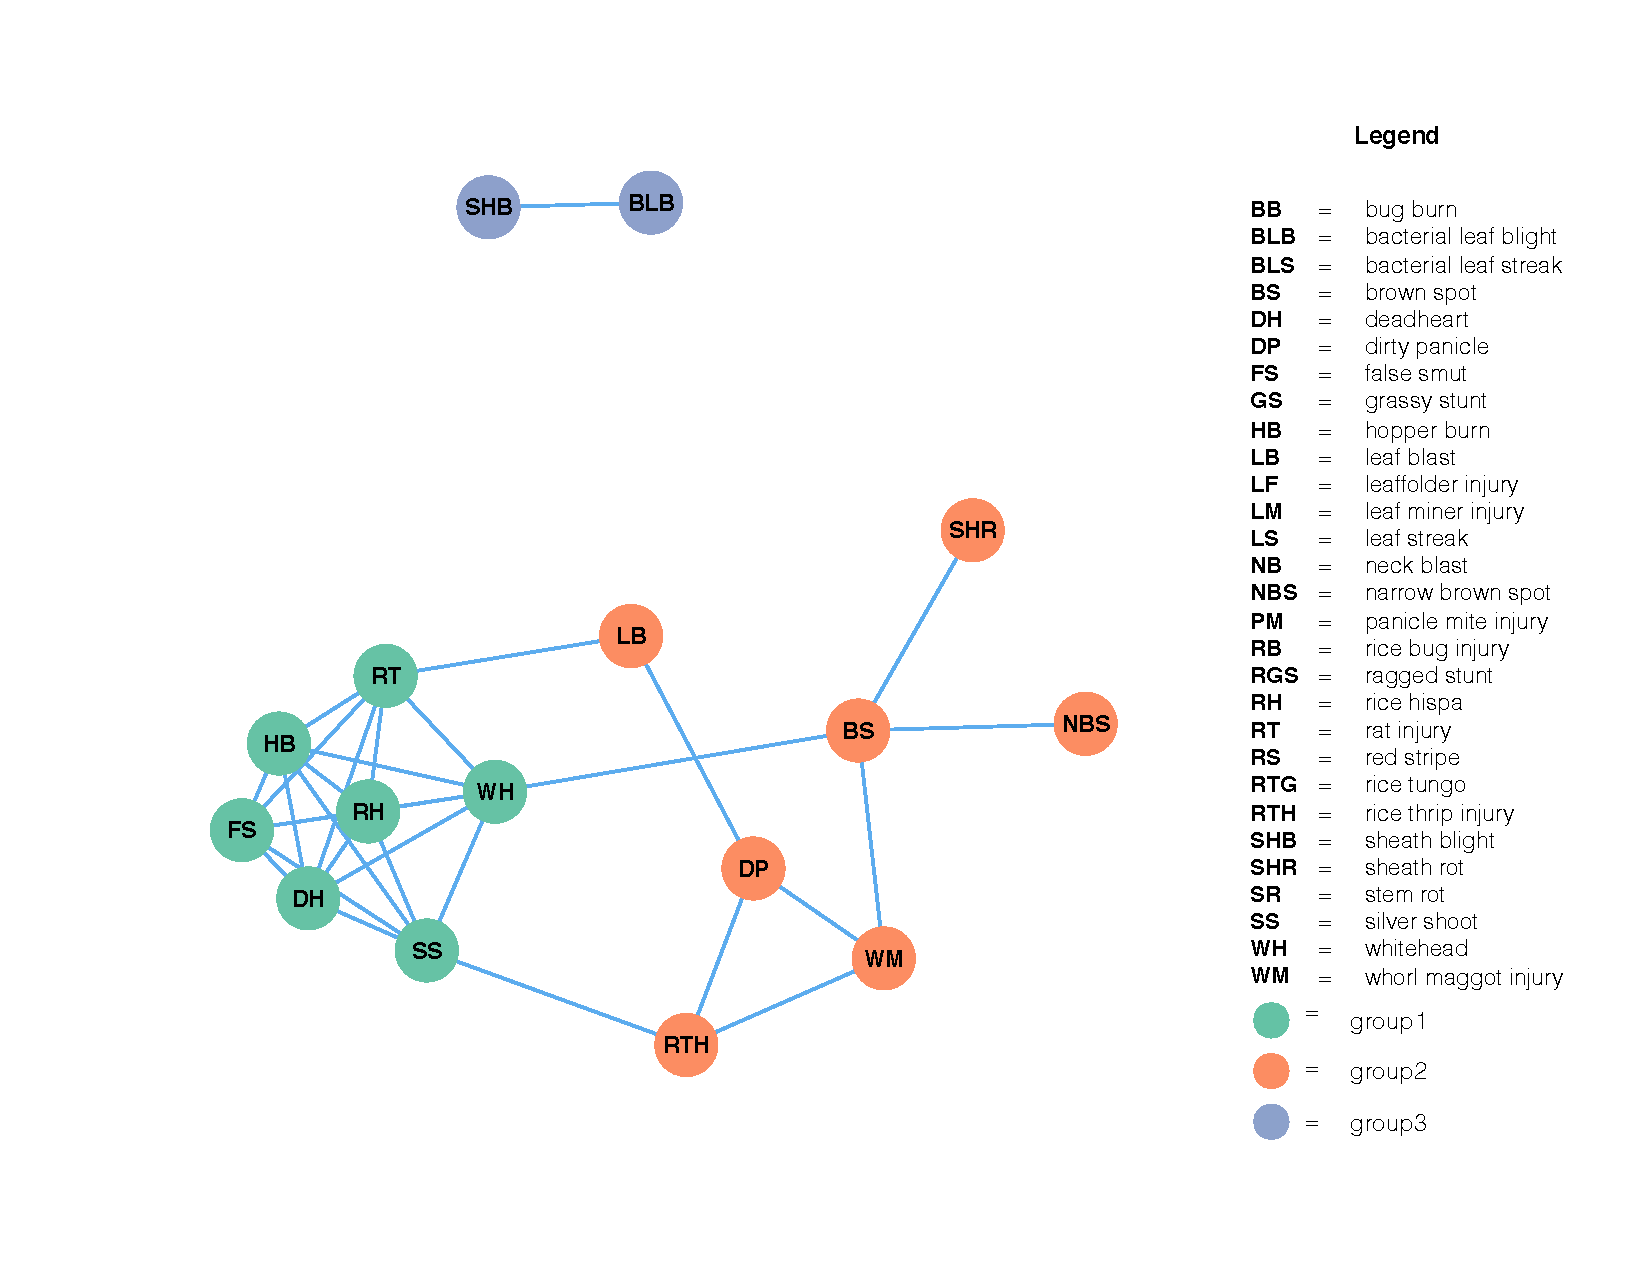
\includegraphics[width = 1\textwidth]{figures/networkTM_ds.pdf}
        \caption{Co-occurrence network of rice injuries in dry season at Tamil Nadu, India. The layout of the network graph is based on the Fruchterman-Reingold algorithm, which places nodes with stronger or more connections closer to each other.}
        \label{fig:networkTM_ds}
    \end{subfigure}
    \begin{subfigure}[b]{1\textwidth}
        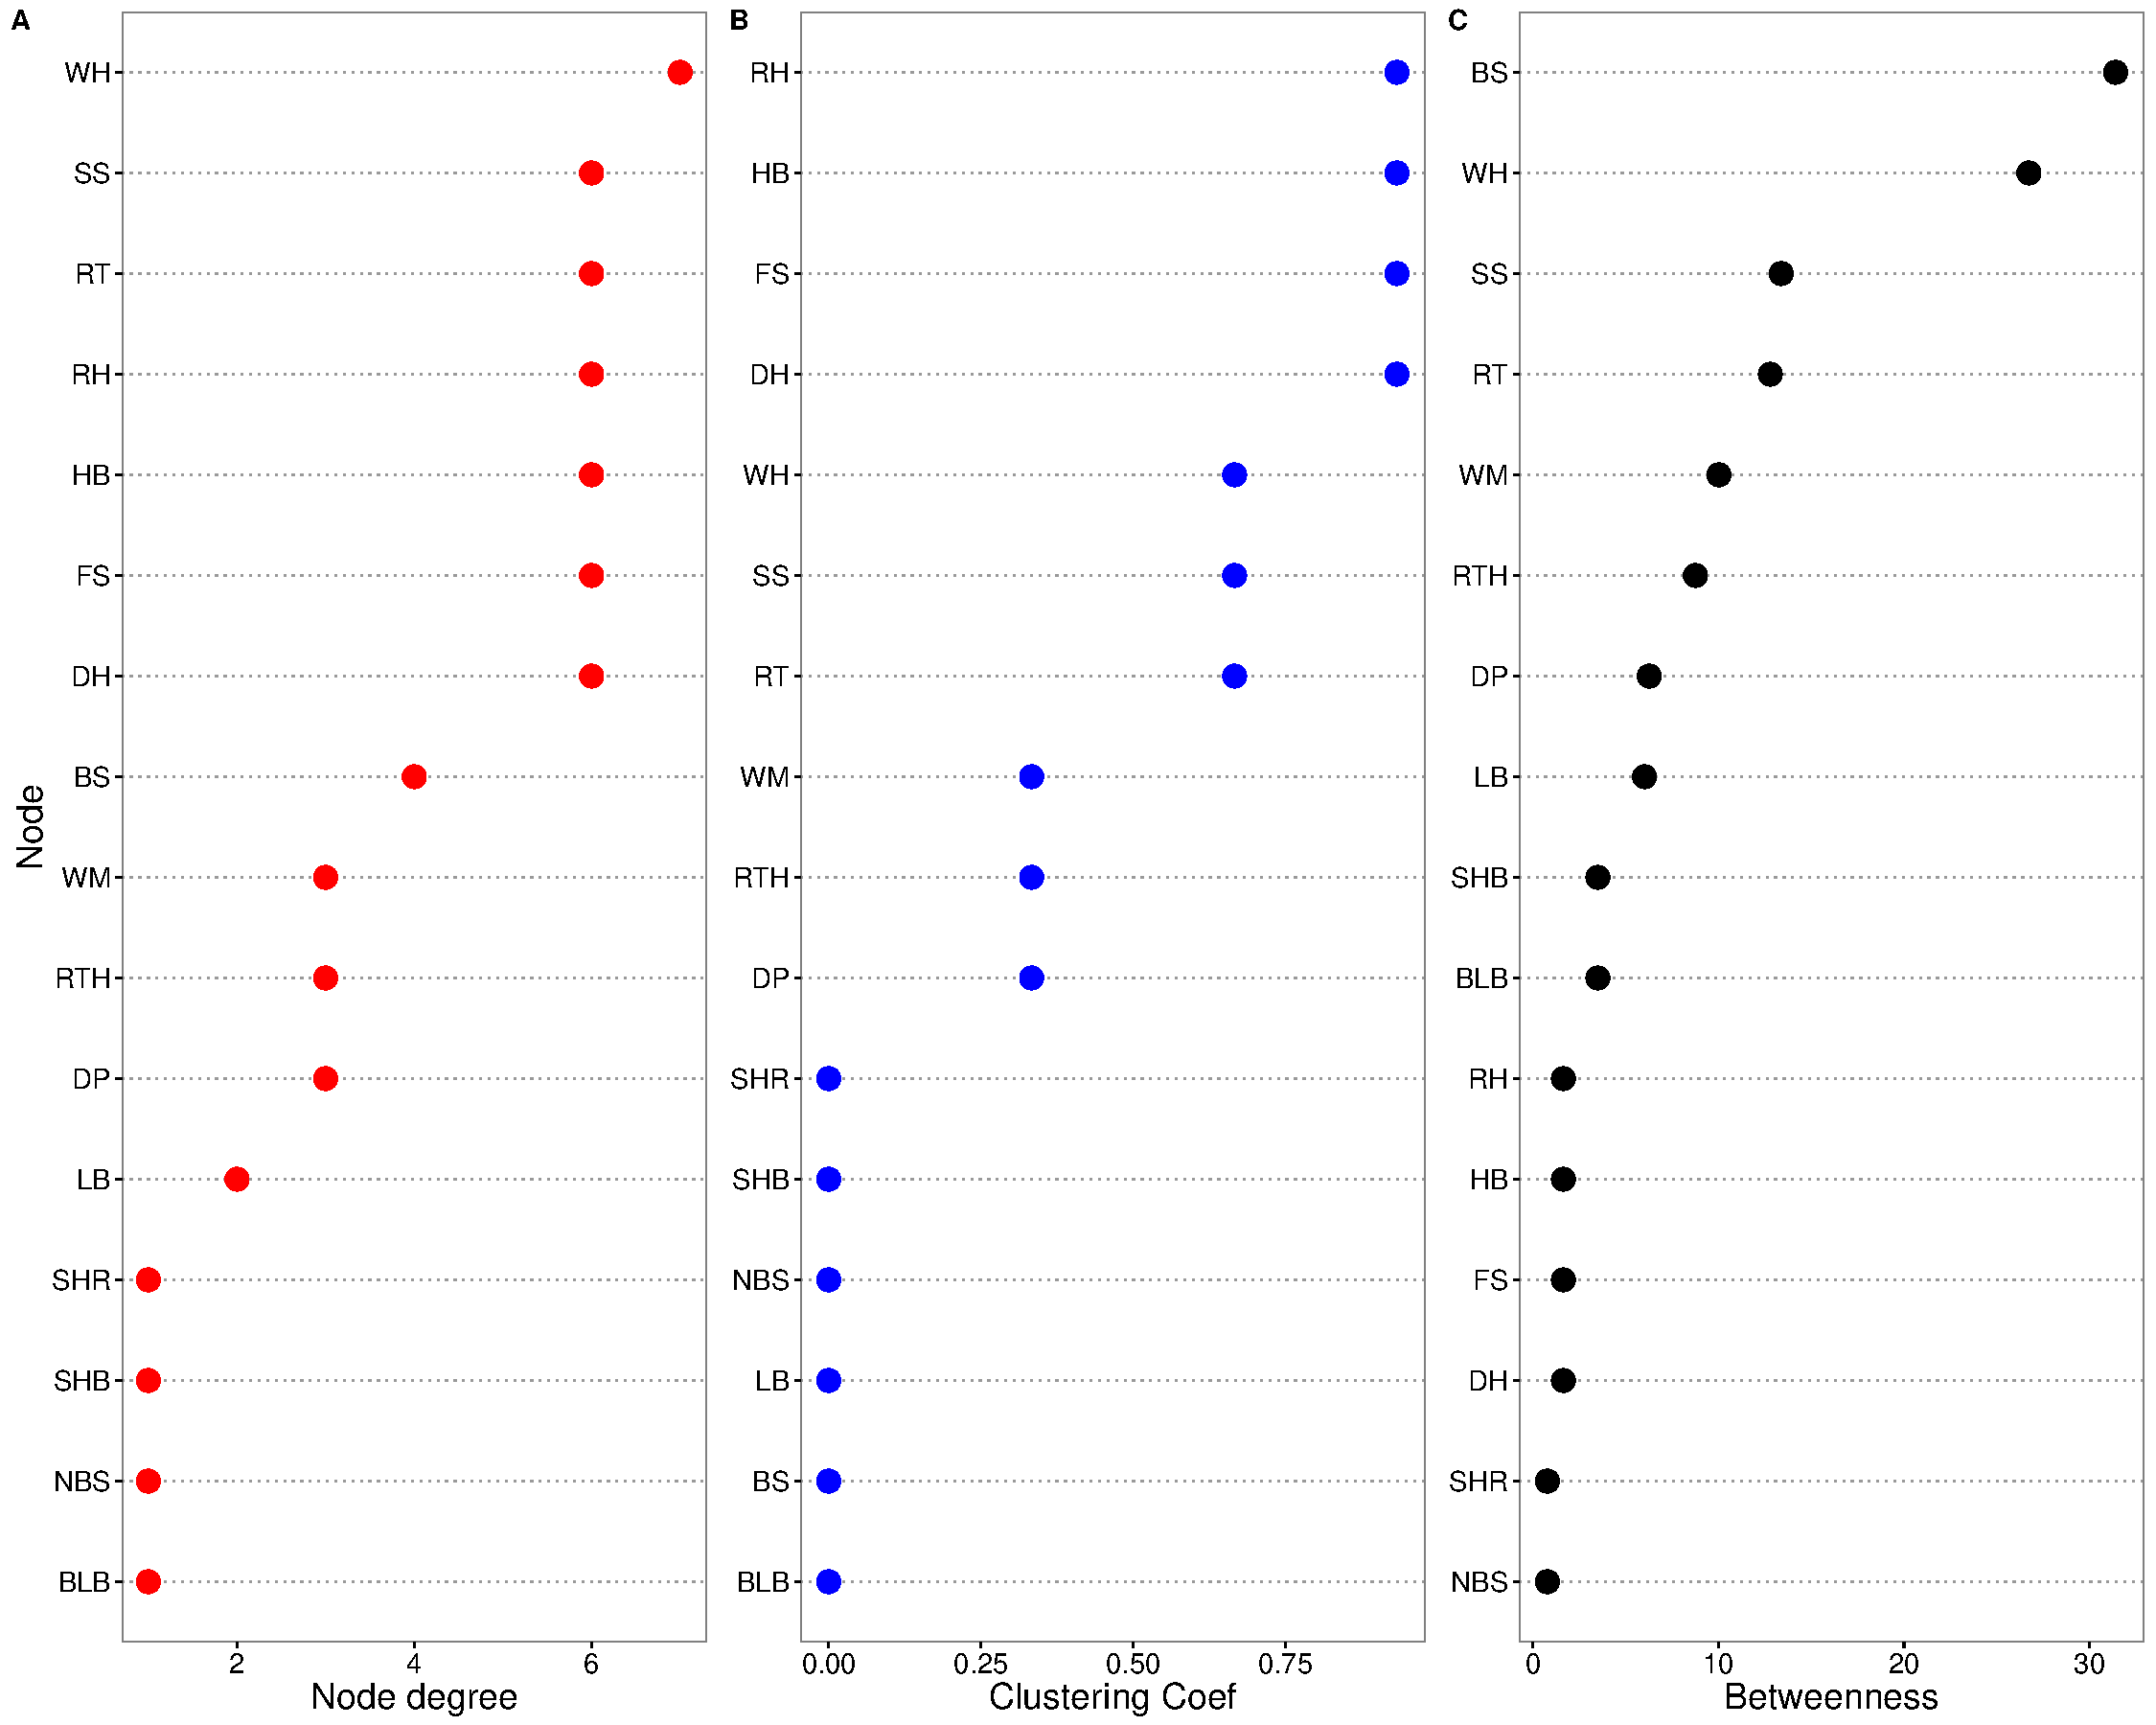
\includegraphics[width = 1\textwidth]{figures/nodepropTM_ds.pdf}
        \caption{Three centrality measures of the nodes in co-occurrence network of rice injuries in dry season at Tamil Nadu, India. A: node degree, B:clustering coefficient, and C:Betweenness, and.}
        \label{fig:nodepropTM_ds}
    \end{subfigure}
    \caption{Rice injuries in dry season in Tamil Nadu, India}
    \label{fig:TM_ds}
\end{figure}

\begin{figure}
    \centering
    \begin{subfigure}[b]{1\textwidth}
        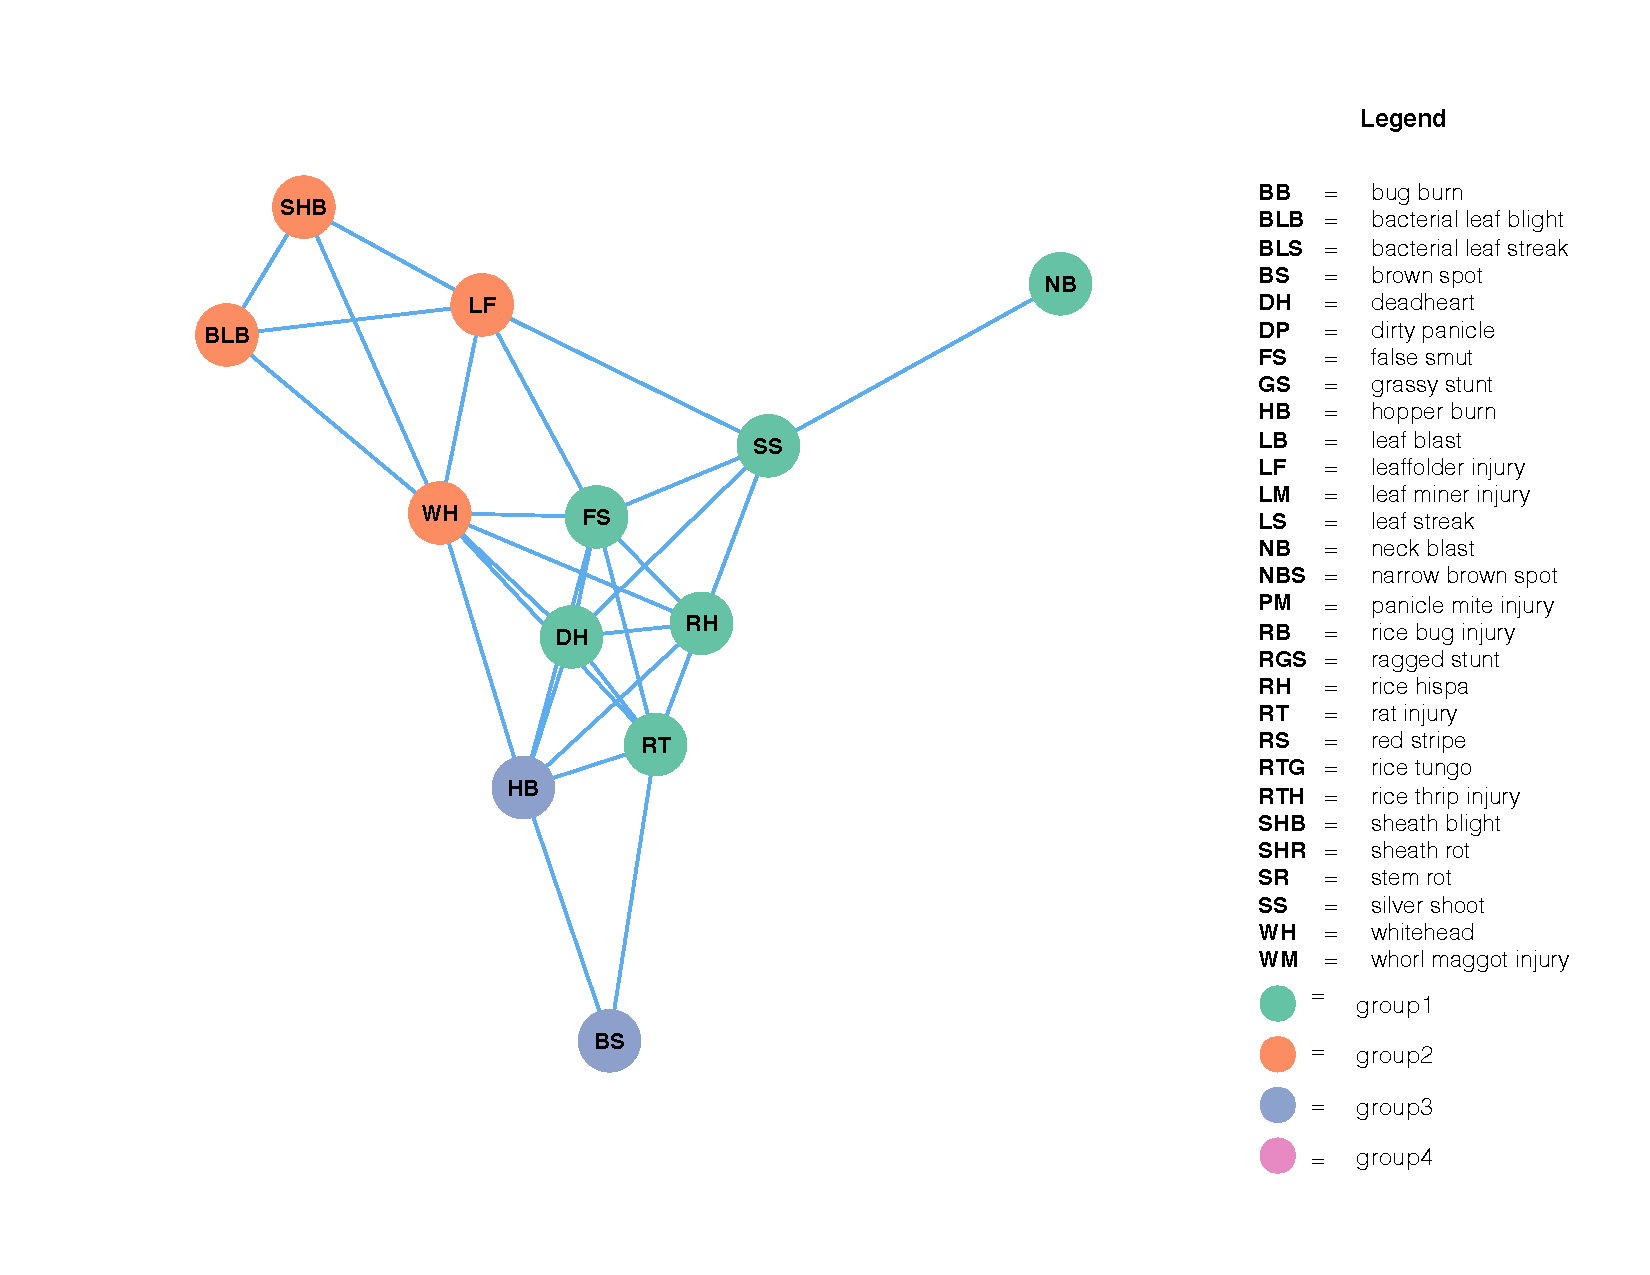
\includegraphics[width = 1\textwidth]{figures/networkTM_ws.pdf}
        \caption{Co-occurrence network of rice injuries in wet season at Tamil Nadu, India. The layout of the network graph is based on the Fruchterman-Reingold algorithm, which places nodes with stronger or more connections closer to each other.}
        \label{fig:networkTM_ws}
    \end{subfigure}
    \begin{subfigure}[b]{1\textwidth}
        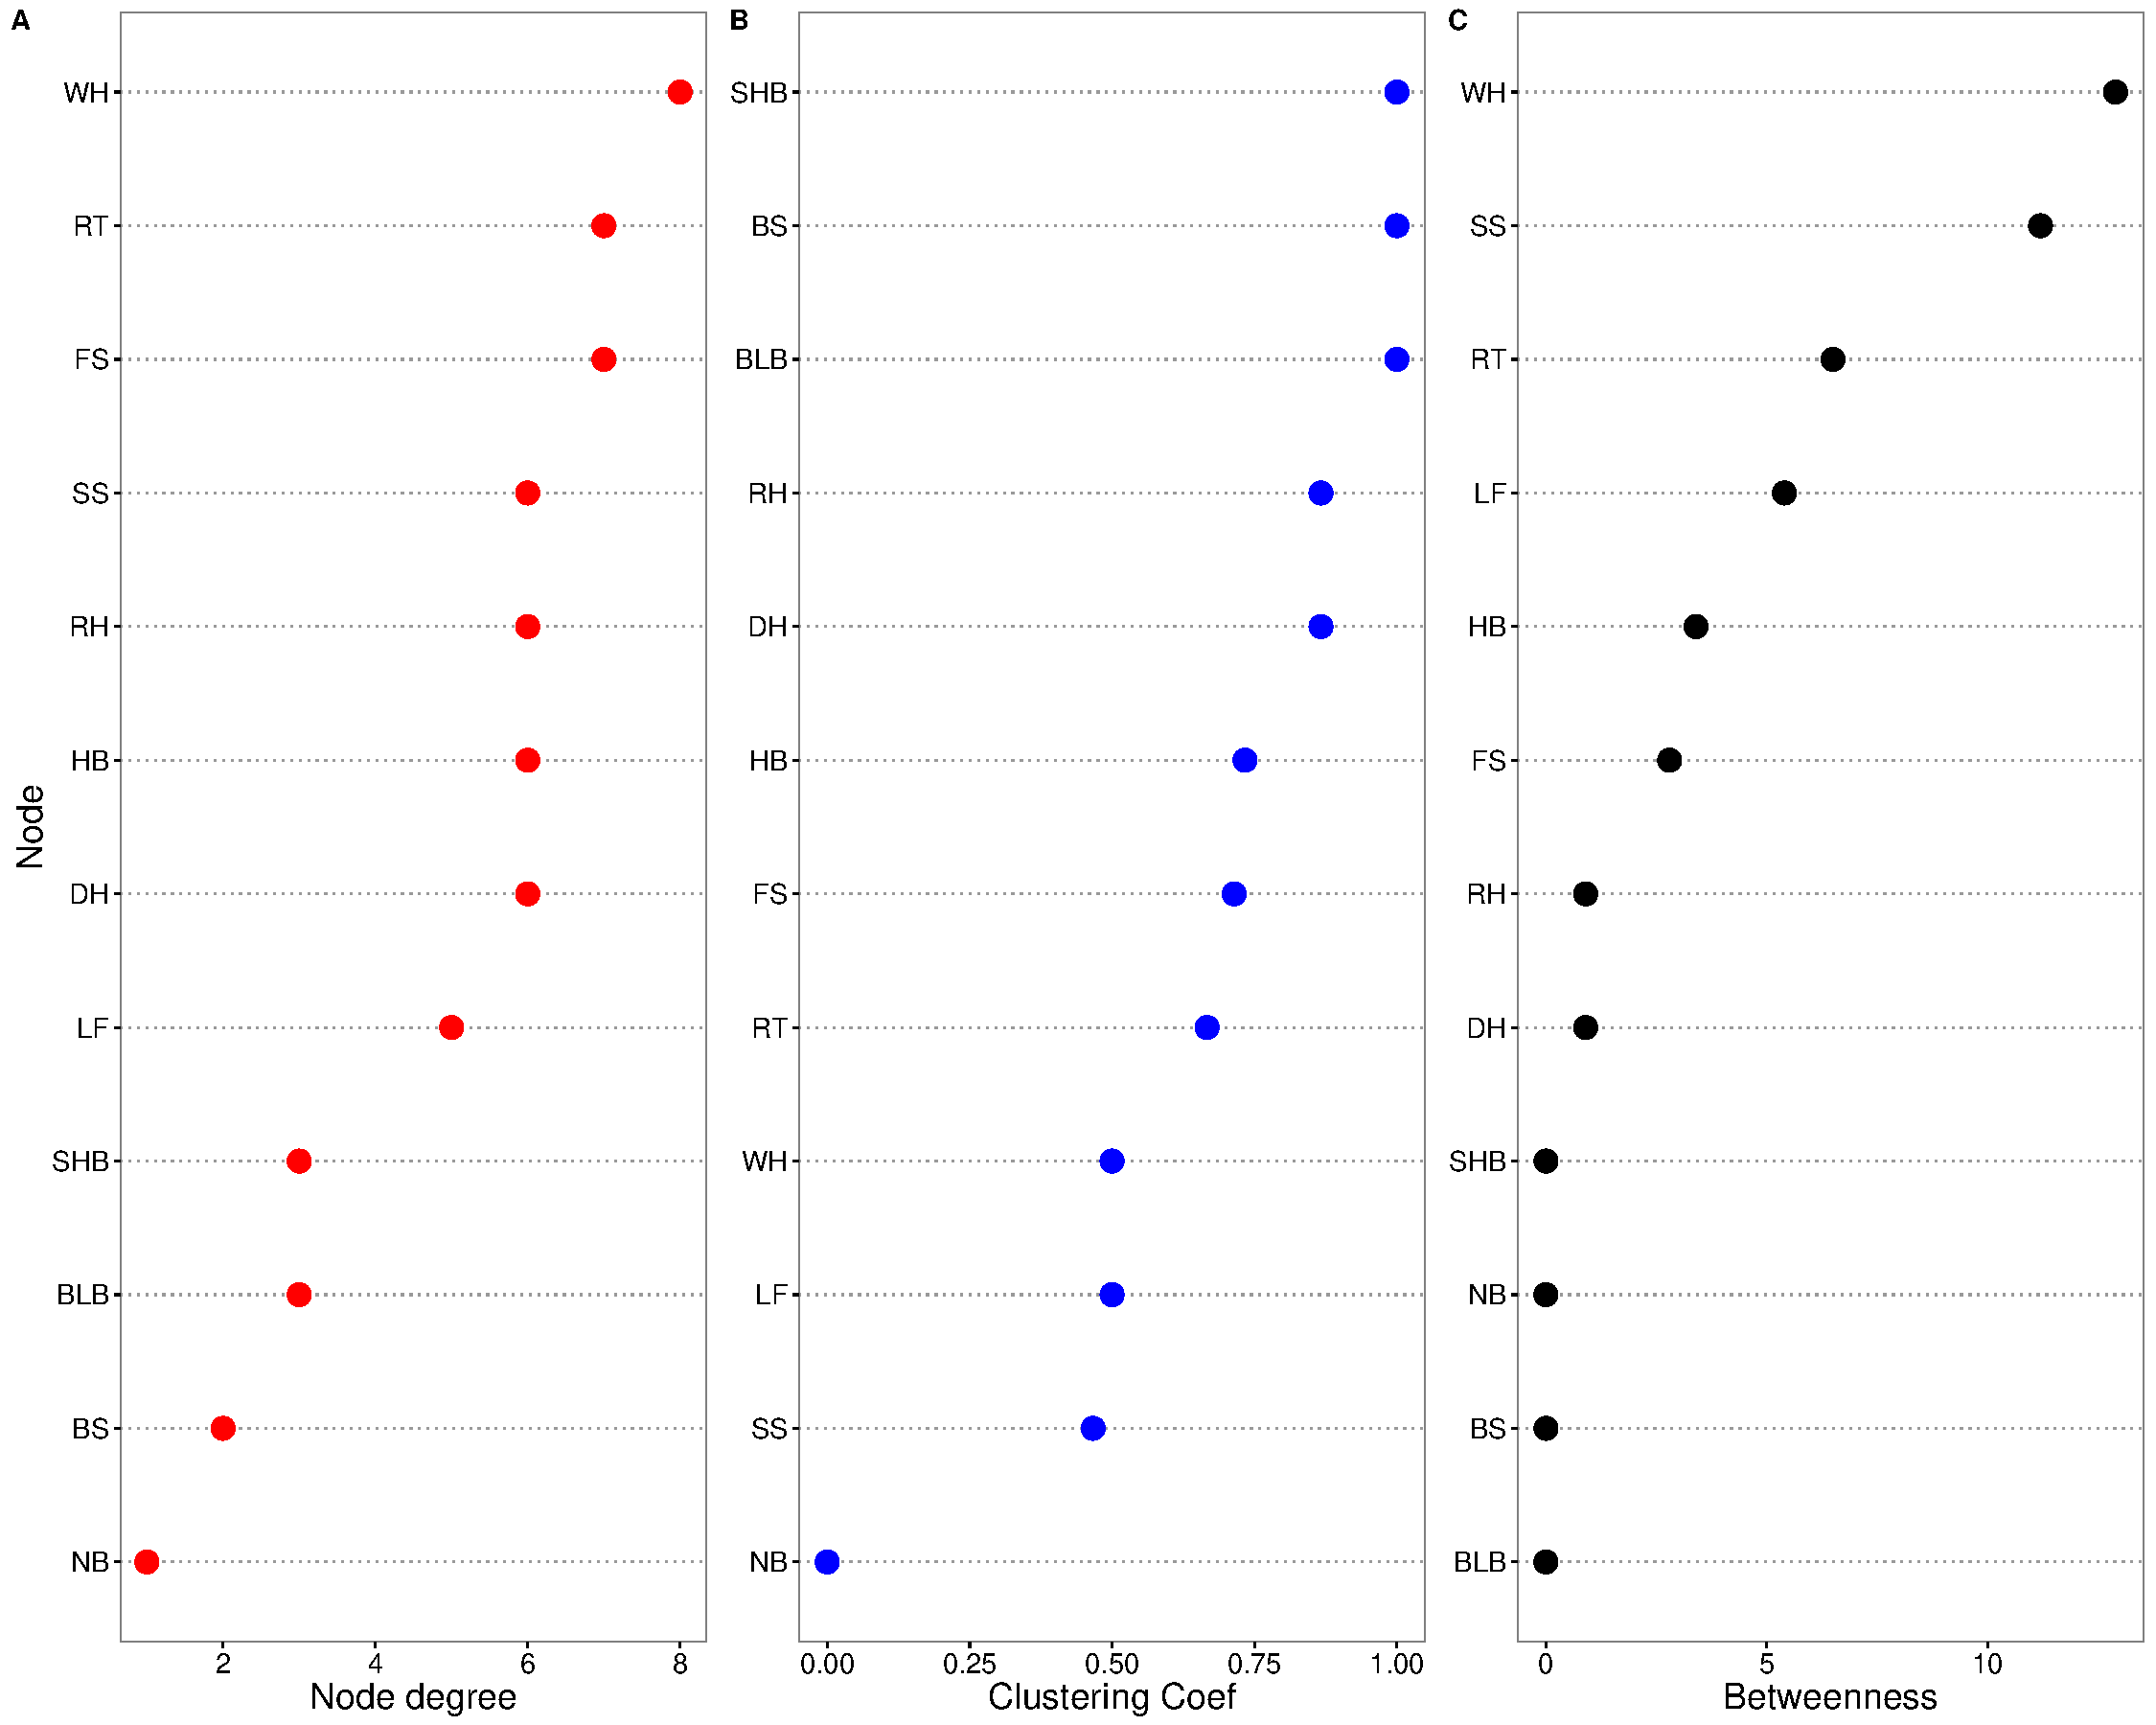
\includegraphics[width = 1\textwidth]{figures/nodepropTM_ws.pdf}
        \caption{Three centrality measures of the nodes in co-occurrence network of rice injuries in wet season at Tamil Nadu, India. A: node degree, B:clustering coefficient, and C:Betweenness, and.}
        \label{fig:nodepropTM_ws}
    \end{subfigure}
    \caption{Rice injuries in wet season in Tamil Nadu, India}
    \label{fig:TM_ws}
\end{figure}

\paragraph{Red Rive Delta, Vietnam}

Co-occurrence network of injury profiles of dry season in Mekong Rive Delta, Vietnam presented 20 injuries (DH, BS, SR, SHB, NBS, SHR, GLH, and WH) with 61 associations. The network reveals the three groups of injury profiles. The group 1 (green) consisted of LB, DP, RB, DH, BS, and FS. The group 2 (orange) was composed of GLH, WPH, SR, WH, BPH, RS, WM. And the group 3 (purple) consisted of RT, NB, SHB, BLB, LF, and NBS. RB in the group 1 has high rank of betweenness and clustering coefficients. The betweenness of injuries in group 2 ranged low to intermediate, but their clustering coefficients are relatively high. This indicated that they are more likely to form complex association within group than between groups. BLB in group 3 and BS in group 1 have high rank of betweenness and they were associated. The average clustering coefficient of group 1 and 3 are smaller than the group 3. So group 1 and 3 are more likely to have chance to form association between the groups.

Co-occurrence network of injury profiles in wet season at Mekong River delta, Vietnam presented 21 injuries (DH, BS, SR, SHB, NBS, SHR, GLH, and WH), and 54 associations. From the structure of this network (Fig), it seems to have three clustered groups base on optimal clustering algorithm. The group 1 (green) is composed of NB, SR, BS, WPH, RS, WM, DH, GLH, FS, RT. The second group (orange) has BLB, BPH, LB, NBS, SHB, SHR, DP. The third group is the smallest groups, which has RB, LF and WH. The members within the first groups are relatively close following the layout, and have similar level of clustering coefficients. SHB and RB, RT, LB have high node degree and betweenness, which are inferred that they have possibility to occur in wet season because they shared many co-occurrence patterns with others. Even though, SHB have high level of betweenness and node degree, but intermediate clustering coefficient.  It connected to the high-betweenness injuries such as RB and RT, where are in different groups. SHB also acted like a ``bridge'', which link the injuries of the group 1 and group 2.


\begin{figure}
    \centering
    \begin{subfigure}[b]{1\textwidth}
        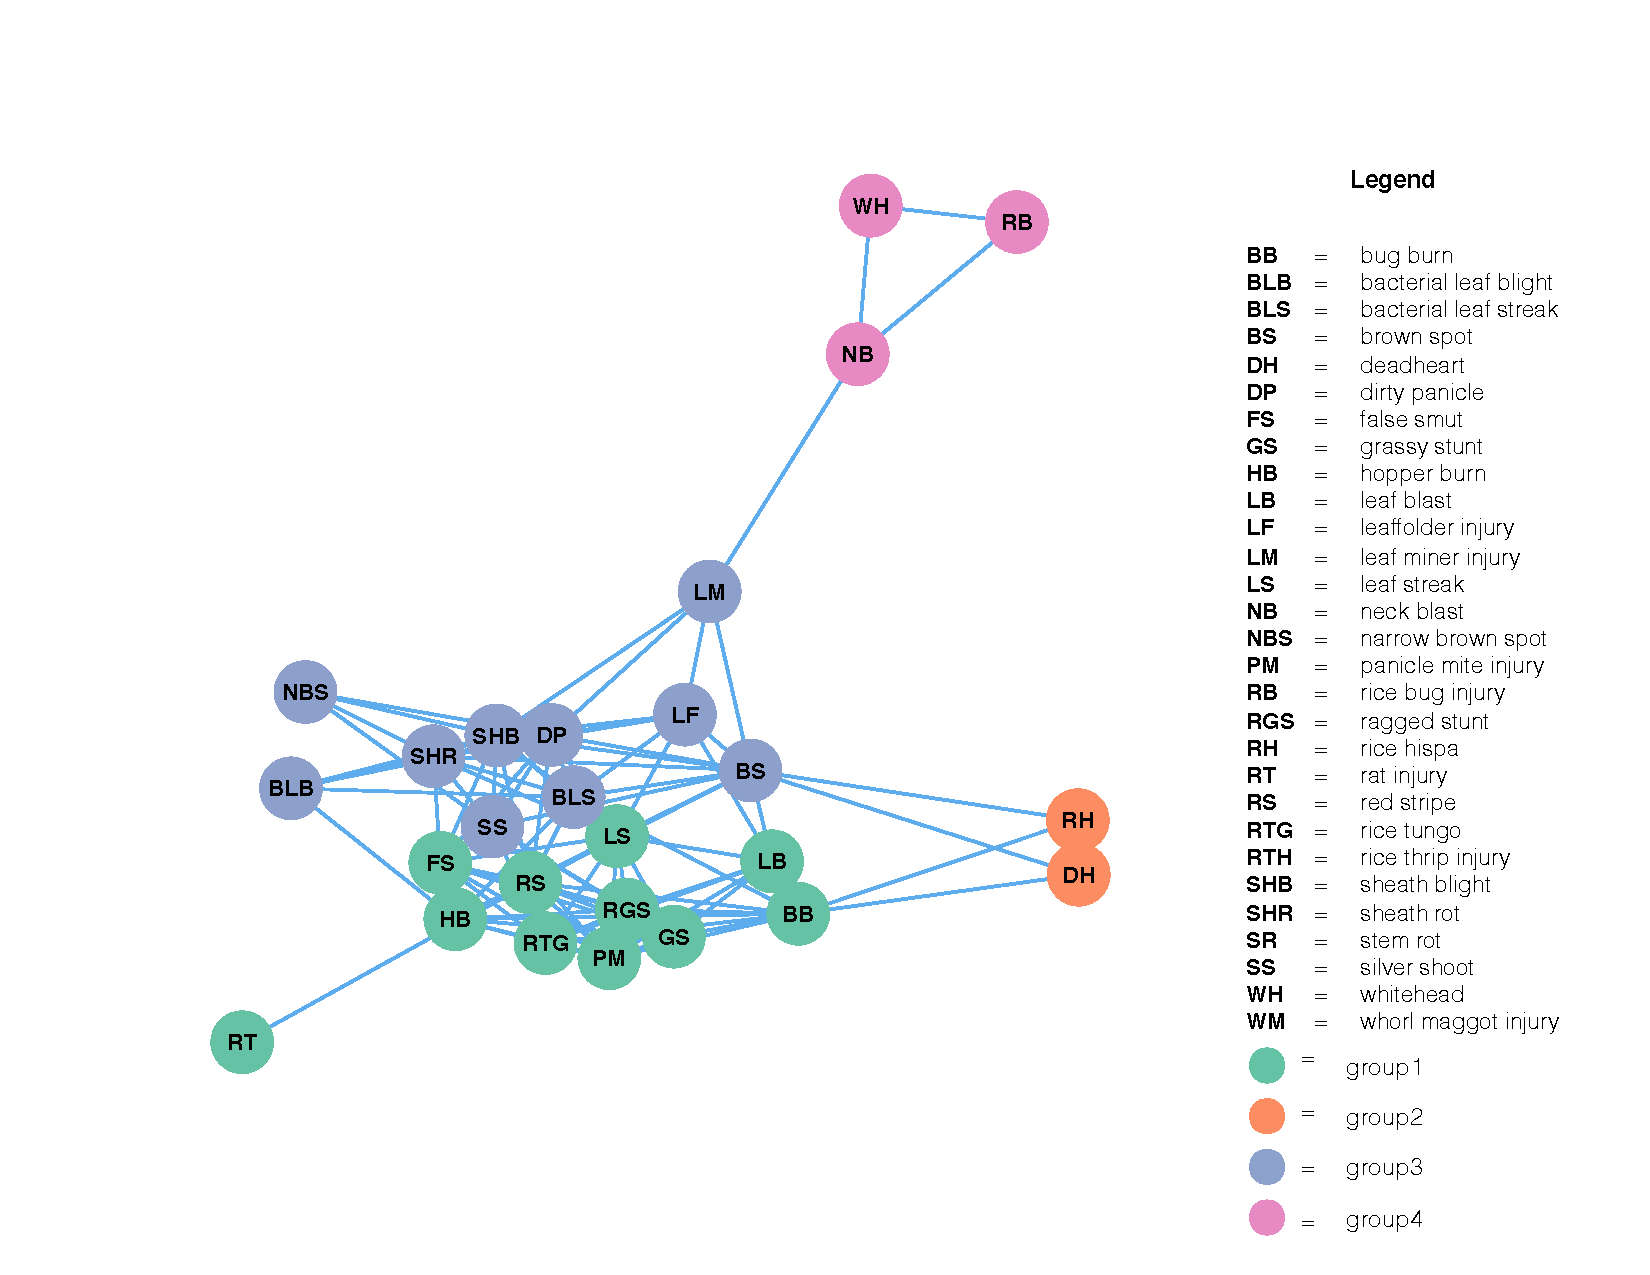
\includegraphics[width = 1\textwidth]{figures/networkWJ_ds.pdf}
        \caption{Co-occurrence network of rice injuries in dry season at West Java, Indonesia. The layout of the network graph is based on the Fruchterman-Reingold algorithm, which places nodes with stronger or more connections closer to each other.}
        \label{fig:networkWJ_ds}
    \end{subfigure}
    \begin{subfigure}[b]{1\textwidth}
        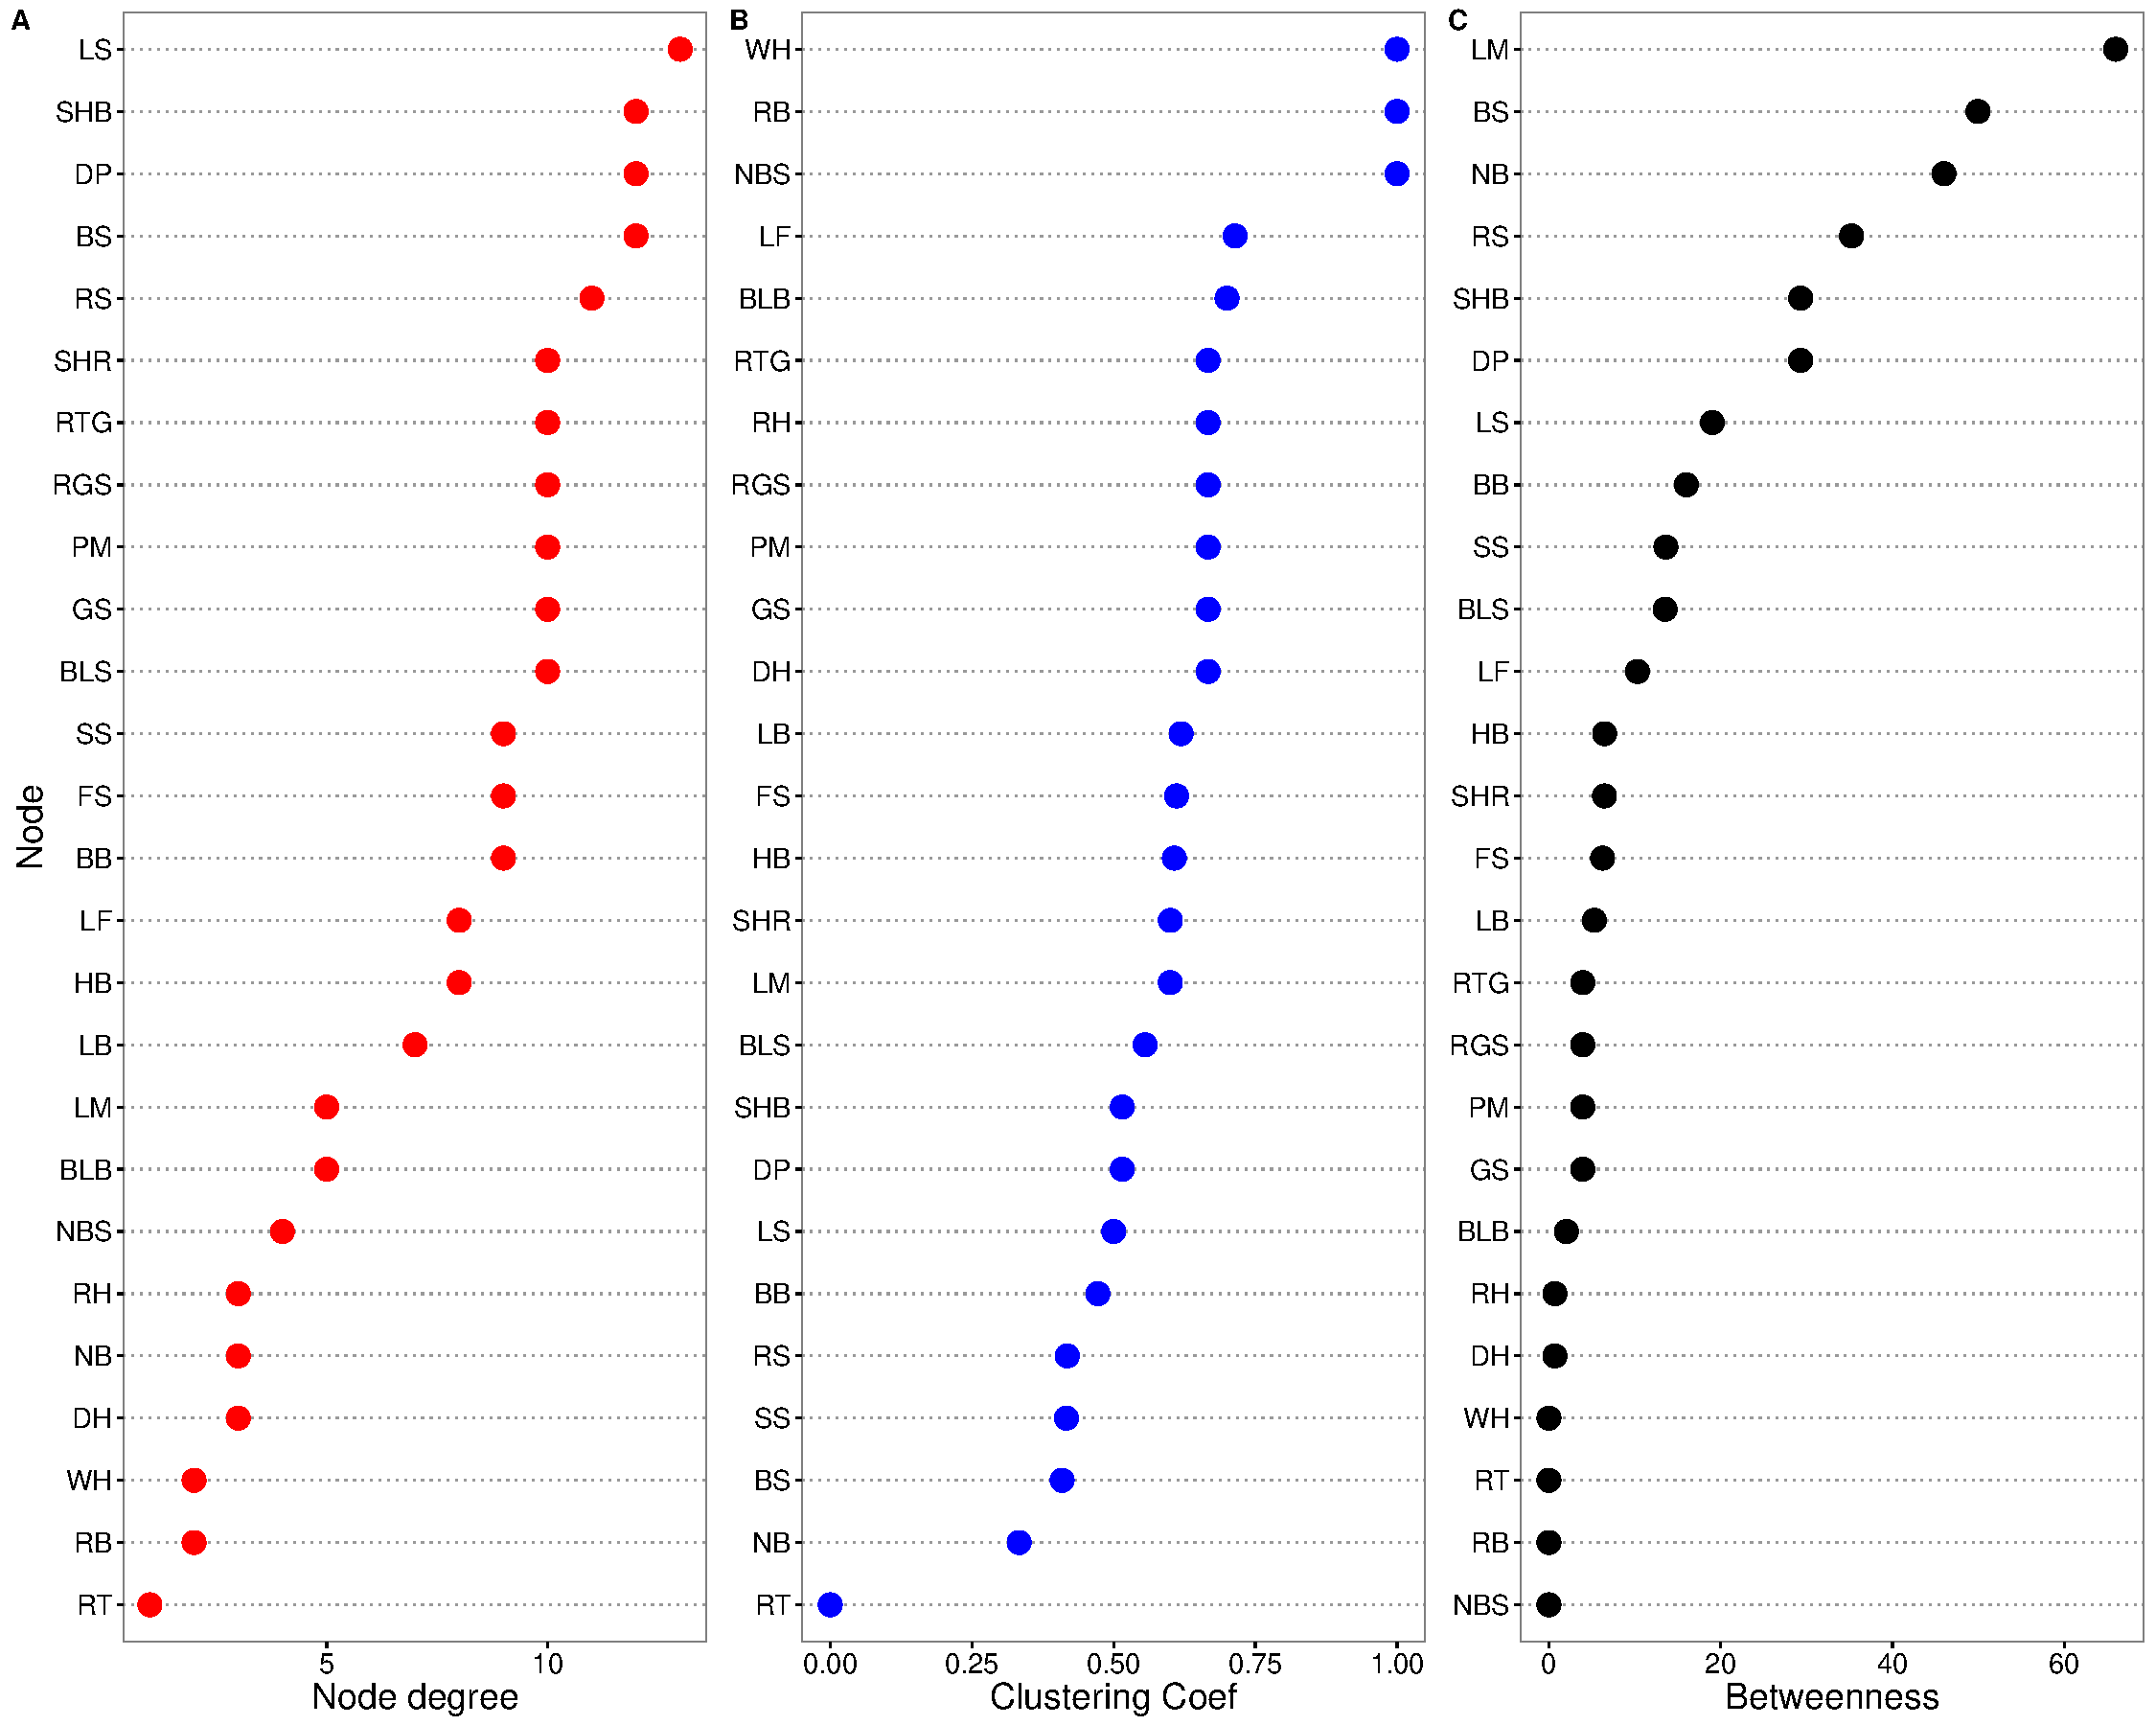
\includegraphics[width = 1\textwidth]{figures/nodepropWJ_ds.pdf}
        \caption{Three centrality measures of the nodes in co-occurrence network of rice injuries in dry season at West Java, Indonesia. A: node degree, B:clustering coefficient, and C:Betweenness, and.}
        \label{fig:nodepropWJ_ds}
    \end{subfigure}
    \caption{Rice injuries in dry season in West Java, Indonesia}
    \label{fig:WJ_ds}
\end{figure}

\begin{figure}
    \centering
    \begin{subfigure}[b]{1\textwidth}
        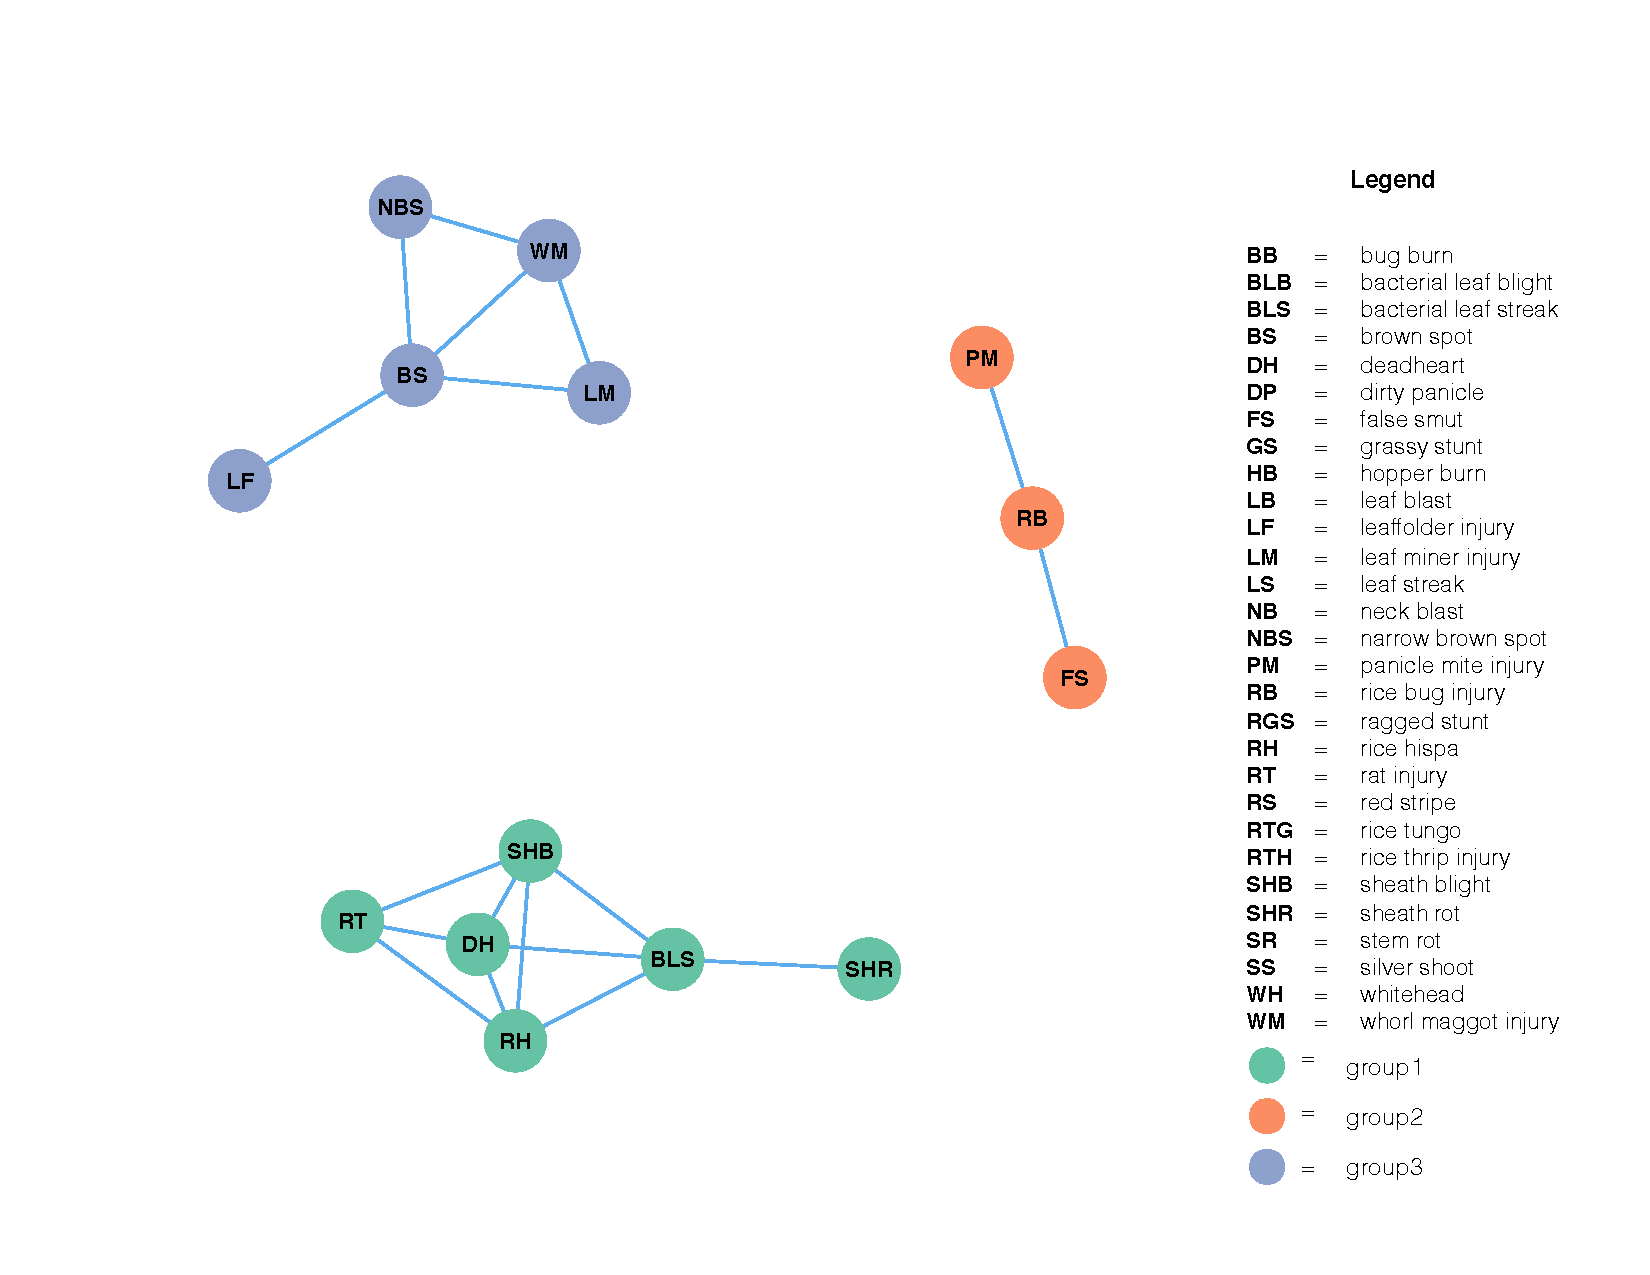
\includegraphics[width = 1\textwidth]{figures/networkWJ_ws.pdf}
        \caption{Co-occurrence network of rice injuries in wet season at West Java, Indonesia. The layout of the network graph is based on the Fruchterman-Reingold algorithm, which places nodes with stronger or more connections closer to each other.}
        \label{fig:networkWJ_ws}
    \end{subfigure}
    \begin{subfigure}[b]{1\textwidth}
        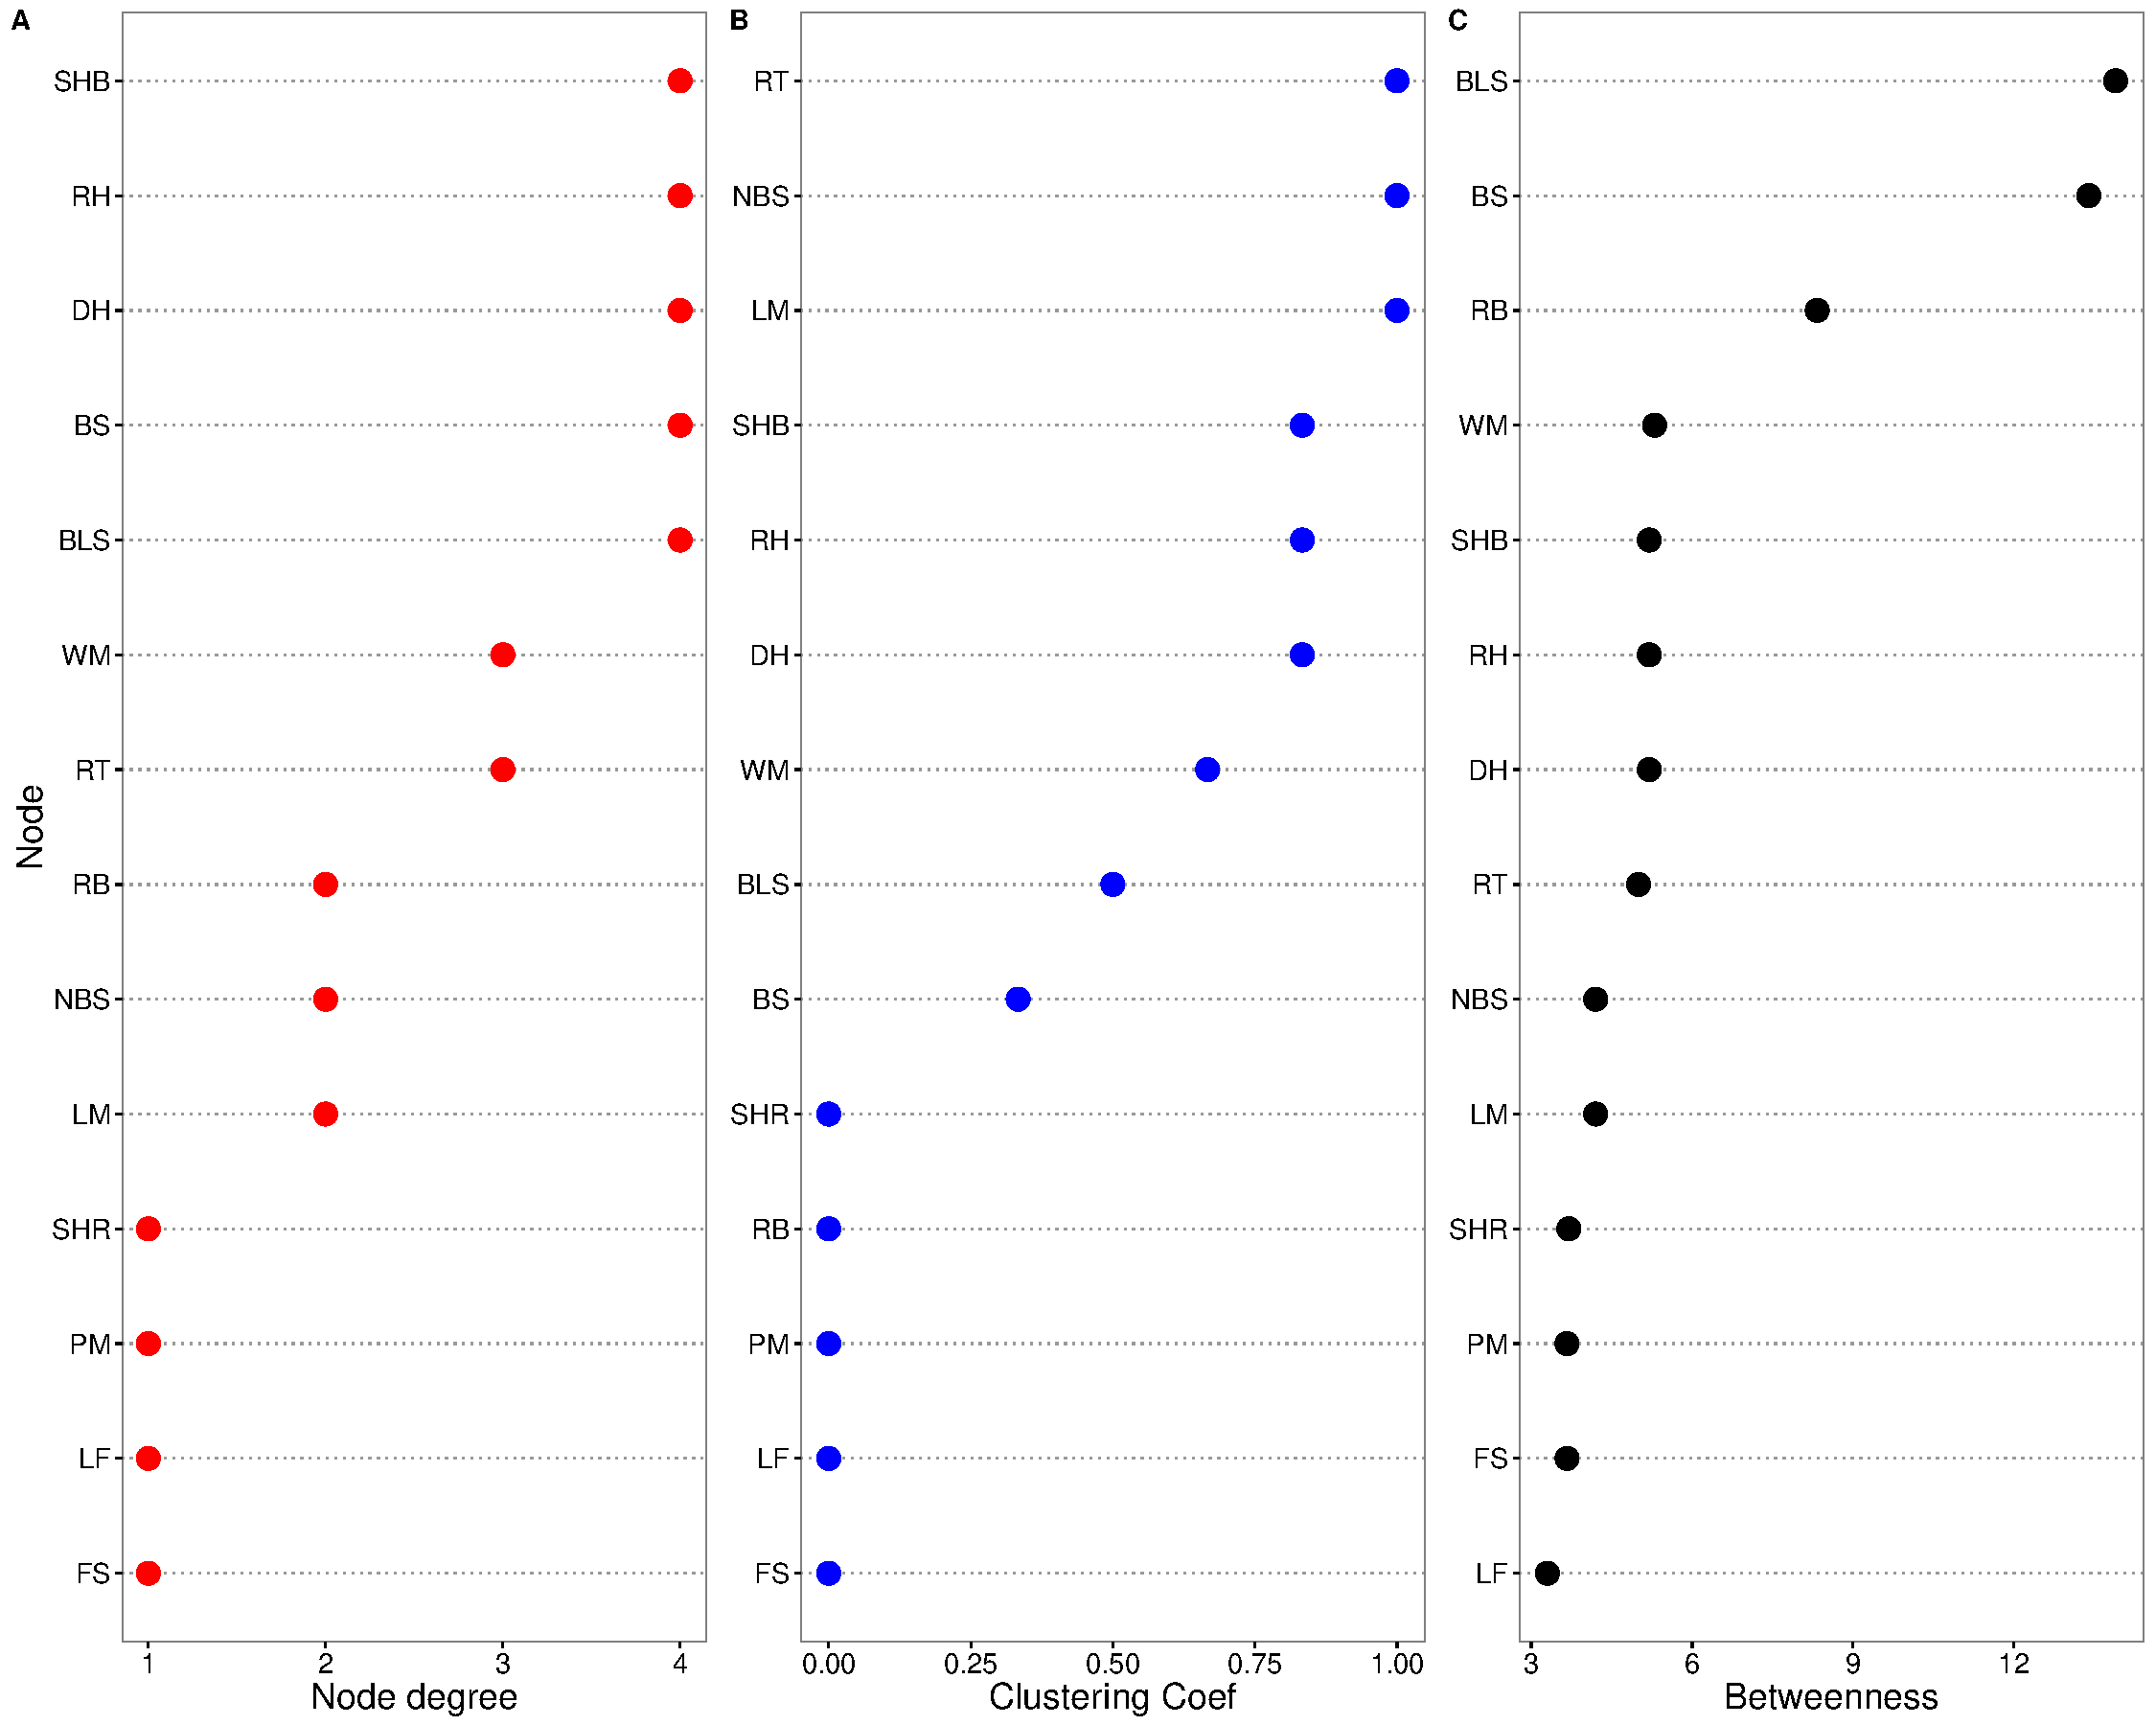
\includegraphics[width = 1\textwidth]{figures/nodepropWJ_ws.pdf}
        \caption{Three centrality measures of the nodes in co-occurrence network of rice injuries in wet season at West Java, Indonesia. A: node degree, B:clustering coefficient, and C:Betweenness, and.}
        \label{fig:nodepropWJ_ds}
    \end{subfigure}
    \caption{Rice injuries in wet season in West Java, Indonesia}
    \label{fig:WJ_ws}
\end{figure}


\subsection{Discussion}

Rice injuries were found commonly in South and South east Asia, but at different levels of incidence. 
Some injuries of this study is relatively low prevalence of areas that have been reported such as leaf blast, brown spot. It could be implied that these injuries strongly depended on locations or climatic conduction to develop, so they were not observed at all locations or seasons during survey were conducted. Another reason is that there are some factors such as the utility of resistance verities in the farmer’s fields surveyed, so we could observe those injuries at low level of incidence. The similar reasoning could explain to many injuries such as BLB, RB, NB, which widely occur in rice growing areas.

From the survey data of rice injuries observed in farmers’ fields, I analyzed the interaction and build the network based on that data. The methods applied for building a co-occurrence network of rice injuries were adapted from ecological studies. Usually, relationships were assessed using Pearson correlation. However, the use of the Pearson correlation coefficient is problematic because it requires the variables are applied with similar measure, and the variable values are normally distributed. Additionally, Pearson correlation can only capture linear relationships. Due to the fact that the assumptions of Pearson correlation are not fit with the survey data. The alternative is provided by using Spearman’s rank correlation coefficient, which is also widely used in ecological studies.

The exploration of co-occurrence networks is a useful method for determining interactions of co- occurring injuries. Network analysis has also suggested important injuries in networks. The important injuries were selected from the node features such as node degree, clustering coefficient, and betweenness. The betweenness represents the importance of the control potential that an injury exerts over the associations of other injuries in the network. The clustering coefficients are indicative of the potential spreading of the incidence of injuries through the network. As activated injury can activate other injuries, a more densely connected network facilitates injury activation \cite{Williams_2014_demonstrating}. In the network of dry season in West Java, Indonesia, BLB and SR can be the targets to be monitored because they have high betweenness, which indicated that they are more likely to present then others injuries.

It is good attempt to detect communities in a network because it can reveal information about the networks that is maybe not easy to detect by simple observation. The communities are groups of nodes that are densely connected among their node members, and slightly connected with the rest of the network.  In this study, we detected node community based on the optimization of the modularity of a sub-network, which is an approach that widely applied in many fields \cite{Liu_2014_Detecting}. Even though, the groups of injury profiles from this study are different from seasons and countries, but they are reasonable because some rice injuries present in some seasons (seasonal occurrence) such as gall midge injury \cite{Krishnaiah_2004_Rice}. The result also showed similar groups of injuries to the patterns of injuries profile from the study of \cite{Savary_2000_Characterization}. 

%SR is also best to be the target because it also associated with the RS, which has high clustering coefficients also because RS is potentially able to be co-found with many other injuries.  BLB also show the association with the injuries, which present high clustering coefficient. Both of BLB and SR are intermediate clustering coefficient., so they are formed concurrence between groups, but less potentially to present complex association. DH and WH are less associated with other injuries, so they are difficult to employ other injuries to. 

It is the good to monitored WM and RB  and SHB also even the GLH has no betweenness, but it has high clustering coefficients, and connected with two high betweenness node. It would be also good target to monitored also because when it present, it also frequency appear together.
We explored the characteristics of rice injury profiles

Communities are groups that are densely connected among their members, and sparsely connected with the rest of the network. Community structure can reveal abundant hidden information about complex networks that is not easy to detect by simple observation. 

With regard to pest management development, understanding that the relationships of rice injuries could simplify pest management decisions. As applied here, the node degree, clustering coefficients, and betweenness described the interaction of injuries in the networks. Therefore, they may be useful in finding a good indicator for monitoring pest in rice fields. High-betweenness node High- clustering coefficient node 

Community structure in complex network can reveal hidden information about complex networks that is maybe not easy to detect by simple observation such as nodes, which are clustered. In this study, we detected node community based on the optimization of the modularity of a sub-network, which is a popular approach \cite{Liu_2014_Detecting}. Even though, the groups of injury profiles from this study are different from seasons and countries, but they are reasonable because some rice injuries present in some seasons (seasonal occurrence) such as gall midge injury \cite{Krishnaiah_2004_Rice}. from the groups of injury profile from \cite{Savary_2000_Characterization}. 



\subsection{Conclusion}

